

\documentclass[12pt]{phd}
%\usepackage{pdfpages}
 %%%%%%%%% PAckage %%%%%%%%%
%% intro 
%\usepackage[utf8]{inputenc}
%\usepackage[british, frenchb]{babel}
%\usepackage[OT1]{fontenc}
\usepackage{enumerate}
\usepackage{smartdiagram}
\usepackage{graphicx,amsmath,amssymb,stmaryrd, amsthm}
%\usepackage{url}
%\usepackage{a4wide}
\usepackage{ulem}
\usepackage{pifont}
\usepackage{amsfonts}
\usepackage{fancyhdr} 
\usepackage{color} % où xcolor selon l'installation
\usepackage{mdframed}
\usepackage{multirow} %% Pour mettre un texte sur plusieurs rangées
\usepackage{multicol} %% Pour mettre un texte sur plusieurs colonnes
\usepackage{tikz}
%\usepackage{graphicx}
\usepackage[absolute]{textpos} 
\usepackage{colortbl}
\usepackage{array}
\usepackage{lineno}
%% JMVA 
\usepackage{enumitem,hyperref,ifthen,dsfont}

%%SAGMB
\usepackage{microtype}
\usepackage{epstopdf}

%%block
\usepackage{multirow}

\setlength\parindent{0pt}
% Functions
\def\independenT#1#2{\mathrel{\rlap{$#1 #2$}\mkern2mu{#1 #2}}}
\DeclareMathOperator*{\argmax}{arg\,max}
\DeclareMathOperator*{\Esp}{\mathbb{E}}
\DeclareMathOperator*{\Var}{\mathbb{V}}
\DeclareMathOperator*{\Cov}{\mathbb{C}\text{ov}}
\DeclareMathOperator*{\prob}{\mathds{P}}
\DeclareMathOperator*{\probt}{\widetilde{\mathds{P}}}


\newcommand{\review}[1]{\textcolor{black}{#1}}
\newcommand{\validSR}[1]{\textcolor{black}{#1}}
\newcommand{\questSR}[1]{\textcolor{black}{[#1]}}
\newcommand{\newmodif}[1]{\textcolor{black}{#1}}
\newcommand{\modif}[1]{\textcolor{black}{#1}}
\newcommand{\remove}[1]{\textcolor{gray}{#1}}
\newcommand\independent{\protect\mathpalette{\protect\independenT}{\perp}}
\newcommand{\STAB}[1]{\begin{tabular}{@{}c@{}}#1\end{tabular}}
\newcommand*\xbar[1]{%
   \hbox{%
     \vbox{%
       \hrule height 0.5pt % The actual bar
       \kern0.5ex%         % Distance between bar and symbol
       \hbox{%
         \kern-0.1em%      % Shortening on the left side
         \ensuremath{#1}%
         \kern-0.1em%      % Shortening on the right side
       }%
     }%
   }%
} 


% Notations pairs
\newcommand\jk{{jk}}

% Notations cal
\newcommand\Ccal{\mathcal{C}}
\newcommand\Ncal{\mathcal{N}}
\newcommand\Pcal{\mathcal{P}}
\newcommand\Tcal{\mathcal{T}}
\newcommand\G{\mathcal{G}}
\newcommand\mt{\widetilde{m}}
\newcommand\St{\widetilde{S}}
\newcommand\mbt{\widetilde{\bf m}}
\newcommand\Sbt{\widetilde{\bf S}}

% Notations bf
\newcommand\gammab{{\boldsymbol{\gamma}}}
\newcommand\betab{{\boldsymbol{\beta}}}
\newcommand\thetab{{\boldsymbol{\theta}}}
\newcommand\Sigmab{{\boldsymbol{\Sigma}}}
\newcommand\cst{\text{cst}}
\newcommand\Ob{{\bf O}}
\newcommand\Hb{{\bf H}}
\newcommand\Mbf{{\bf M}}
\newcommand\Qbf{{\bf Q}}
\newcommand\Abf{{\bf A}}
\newcommand\Wbf{{\bf W}}
\newcommand\Mb{{\bf M}}
\newcommand\Qb{{\bf Q}}
\newcommand\Wb{{\bf W}}
\newcommand\Xb{{\bf X}}
\newcommand\xb{{\bf x}}
\newcommand\Yb{{\bf Y}}
\newcommand\Zb{{\bf Z}}
\newcommand\zb{{\bf z}}

% Notations tilde
\newcommand\Pt{\widetilde{P}}
\newcommand\pt{\widetilde{p}}
\newcommand\et{\widetilde{\mathds{E}}}
\newcommand\e{{\mathds{E}}}
% TikZ
\newcommand{\nodesize}{0.4em}
\newcommand{\edgeunit}{6*\nodesize}
\tikzstyle{covariate}=[draw, rectangle, minimum width=\nodesize, minimum height=\nodesize, inner sep=0, color=black]
\tikzstyle{covmiss}=[draw, minimum width=\nodesize, minimum height=\nodesize, inner sep=0, color=gray, text=gray]
\tikzstyle{observed}=[draw, circle, minimum width=\nodesize, inner sep=0, color=black]
\tikzstyle{edge}=[-, line width=1pt, color=black]
\tikzstyle{edgemiss}=[-, line width=1pt, dashed, color=gray]
\tikzstyle{basic}=[draw, circle, minimum width=\nodesize, inner sep=0, color=black, fill=black]

\newtheorem{theorem}{Theorem}[chapter]
\newtheorem{prop}[theorem]{Proposition}
%\newtheorem{corollary}[theo]{Corollary}
\newtheorem{lemma}[theorem]{Lemma}
\newtheorem{definition}{Definition}[chapter]
\newtheorem{remark}{Remark}[chapter]
\newtheorem{example}{Example}[chapter]
\DeclareMathOperator{\sign}{sign}
\def\lambdaMax{\lambda_{\rm{max}}}
\def\lambdaMin{\lambda_{\rm{min}}}
\newcommand{\tr}[1]{\ensuremath{\rm tr}\left( #1 \right)}
\newcommand{\ve}{\ensuremath{\rm vec}}
 

%\pagestyle{empty}
 
\numberwithin{figure}{chapter}
\backgroundsetup{contents={}}
\newcommand{\nocontentsline}[3]{}
\newcommand{\tocless}[2]{\bgroup\let\addcontentsline=\nocontentsline#1{#2}\egroup}
\setcounter{chapter}{-1}

\begin{document}
\frontmatter

\begin{titlepage}


%\thispagestyle{empty}

\newgeometry{left=7.5cm,bottom=2cm, top=1cm, right=1cm}

\tikz[remember picture,overlay] \node[opacity=1,inner sep=0pt] at (-28mm,-135mm){
\includegraphics{Bandeau_UPaS.png}};

% fonte sans empattement pour la page de titre
\fontencoding{T1}

\fontfamily{fvs}\fontseries{m}\selectfont


%*****************************************************
%******** NUMÉRO D'ORDRE DE LA THÈSE À COMPLÉTER *****
%******** POUR LE SECOND DÉPOT                   *****
%*****************************************************

\color{white}

\begin{picture}(0,0)

\put(-150,-735){\rotatebox{90}{NNT: 2020UPASA000}}
\end{picture}
 
%*****************************************************
%**  LOGO  ÉTABLISSEMENT PARTENAIRE SI COTUTELLE
%**  CHANGER L'IMAGE PAR DÉFAUT **
%*****************************************************
%\vspace{-10mm} % à ajuster en fonction de la hauteur du logo
%\flushright 
\includegraphics[scale=1]{logo2.png}




%*****************************************************
%******************** TITRE **************************
%*****************************************************
\flushright
\vspace{10mm} % à régler éventuellement
\color{Prune}
\fontfamily{fvs}\fontseries{m}\fontsize{22}{26}\selectfont
Inférence de réseaux à partir de données d'abondances incomplètes

%*****************************************************

%\fontfamily{fvs}\fontseries{m}\fontsize{8}{12}\selectfont
\normalsize
\vspace{1.5cm}

\color{black}
\textbf{Thèse de doctorat de l'Université Paris-Saclay}

\vspace{15mm}

École doctorale n$^{\circ}$ 574, mathématiques Hadamard (EDMH)\\
\small Spécialité de doctorat : Mathématiques appliquées\\
\footnotesize Unité de recherche : Université Paris-Saclay, AgroParisTech, INRAE, UMR MIA-Paris, 75005, Paris, France.\\
\footnotesize Référent :  Faculté des sciences d’Orsay
\vspace{15mm}

\textbf{Thèse présentée et soutenue à Paris, le 20/10/2020, par}\\
\bigskip
\Large {\color{Prune} \textbf{Raphaëlle MOMAL}}


%************************************
\vspace{\fill} % ALIGNER LE TABLEAU EN BAS DE PAGE
%************************************

\flushleft \small \textbf{Composition du jury:}
\bigskip



\scriptsize
\begin{tabular}{|p{8cm}l}
\arrayrulecolor{Prune}
\textbf{Viet-Chi Tran} &   Président\\ 
Professeur des Universités, Université Gustave-Eiffel & \\
\textbf{Florence Forbes} &  Rapportrice \\ 
Directrice de recherches, INRIA Bordeaux   &   \\ 
\textbf{Otso Ovaskainen} &  Rapporteur \\ 
Professor, University of Helsinky  &   \\ 
\textbf{Christophe Ambroise} &  Examinateur \\ 
Professeur des Universités, Université Paris-Saclay  &   \\ 
\textbf{Camille Coron} &  Examinatrice \\ 
Titre, Affiliation   &   \\ 
\textbf{Stéphane Dray} &  Examinateur \\ 
Titre, Affiliation   &   \\ 
\textbf{Stéphane Robin} &   Examinateur\\ 
Directeur de recherches, Université Paris-Saclay & \\

\end{tabular} 

\medskip
\begin{tabular}{|p{8cm}l}\arrayrulecolor{white}
\textbf{Stéphane Robin} &   Directeur\\ 
Directeur de recherches, Université Paris-Saclay & \\
\textbf{Christophe Ambroise} &   Codirecteur\\ 
Professeur des Universités, Université Paris-Saclay  &   \\ 


\end{tabular} 


\end{titlepage}

 \clearemptydoublepage
\setcounter{tocdepth}{1}
\selectlanguage{english}
\dominitoc
\nomtcrule
 \clearemptydoublepage
 \newpage
 \chapter*{Remerciements}
 
  Merci Stéphane et Christophe pour ces trois dernières années (et un peu plus), durant lesquelles vous avez su accueillir mes doutes et mes erreurs avec patience et grand renforts de sourires. Ça a été un grand honneur de travailler avec vous deux, j'ai énormément appris et j'espère qu'on aura l'occasion de faire durer le plaisir encore un peu.\\


 Je remercie Florence Forbes et Otso Ovaskainen d'avoir rapporté cette thèse. Je remercie également Camille Coron, Chi Tran et Stéphane Dray d'avoir accepté de faire partie du jury.  Merci  aussi à Matthieu Authier et Mahendra Mariadassou pour des discussions intéressantes et enrichissantes.\\
 
 Je n'aurais jamais cru faire une thèse en mathématiques un jour. Enfin si, quand François Coquet m'a amené doucement à l'idée. Merci François de m'avoir poussée à ne pas me contenter de ce que j'avais sous les yeux. J'ai vraiment pris ma décision lors de mon premier contact avec la recherche. Merci à Andrea Rau d'avoir fait de cette expérience une révélation.\\

 
 On m'avait prévenu que j'arrivais dans un labo un peu spécial, un labo pas comme les autres.  L'Agro c'est comme une grande bourrasque d'été. Ça réchauffe, ça fait rire, ça décoiffe. Un lieu chaleureux et dynamique, peuplé de gens bourrés de talents et d'humour. Je remercie du fond du coeur toute cette grande famille, en commençant par les parents : Liliane, Éric, Céline, Julien, Marie-Laure, Sophie, Isabelle, Laure, Julie, Sarah, Pierre B,  Tristan, Maud, Jade, Joon, Erica, Christelle, Christophe D, Marie-Pierre. Un énorme merci aux  générations précédentes \sout{d'enfants} de doctorants que j'ai eu la chance de croiser : Anna, Marie C, Paul, Yann, Mathieu, Thimothée et Rana. \\
 
Annarosa, Martina, merci les filles !! Merci d'avoir rendu ce dernier bureau drôle et studieux juste ce qu'il faut, je n'aurais voulu partager les (quelques) craquages de dernière année avec personne d'autre. Ne changez rien vous êtes parfaites. Merci Claire pour tous tes passages (trop courts), pour les orangettes, et ces magnifiques (c'est le mot !) duos entre flûtistes. Je te souhaite le meilleur pour tes prochaines aventures. Antoine, merci de diffuser la bonne parole de R tidy, grâce à toi nous sommes de plus en plus nombreux dans la paroisse. Merci Félix pour ces moments de calme autour d'un bon thé, et ces week-ends en Bourgogne dont on se souviendra longtemps (qui a dit qu'une chaudière était nécessaire ? Une cheminée suffit !). Merci Saint-Clair de nous rappeler qu'on peut avoir vécu mille vies avant de se lancer dans une thèse ; amuse-toi bien dans la suite de cette aventure. Je remercie aussi les nouveaux que je n'ai pas eu le temps de mieux connaître : Wencan, Gaspard, Tâm et Marina. À vous la suite ! \\
Gabriel (j'ai failli te mettre dans les doctorants, je sais que ça te fait plaisir), merci pour toutes ces histoires, pour tes imitations d'hamsters et de poires astringentes, pour ces moments d'éclats sur isc, et pour ton expertise dans tous les domaines de la vie qu'en tant que petit doctorant on ne comprends pas toujours très bien. Pierre G merci pour tes éclats de voix (notamment de Julien Clerc), pour ta \sout{patience} tolérance à puyo puyo et pour nous rappeler qu'il est urgent de rire.  


Marie est une personne extraordinaire qui a le pouvoir d'augmenter le niveau de bonheur autour d'elle. Elle a l'effet secondaire d'induire une accoutumance assez sévère. Ayant la chance d'avoir partagé son bureau pendant 2 ans, puis d'avoir récidivé aux cours de théâtre, aux soirées et aux week-ends en Normandie, je suis complètement addict, je l'avoue sans rougir. Mais ce traitement de fond fait de moi un être humain plus heureux.  Alors merci Marie, je serais toujours là pour toi. 


Un grand merci à Charles (et les chichis), Luc, Nico et Joachim pour vos folies respectives. Marine, après toutes ces années tu continues à me suivre. Merci pour toutes ces aventures, hâte de la prochaine ! Merci aussi aux copains sans lesquelles je ne serais pas là aujourd'hui :  Jihane, Syrielle, Florian, Rocket, Clément et Laure.


Je remercie enfin ma famille sur laquelle je sais pouvoir compter. Merci beaucoup à mes frères et soeurs pour vos encouragements, Alain, Hélène, Ludo, les belles-soeurs de choc au top Sylvie et Amélie. Je remercie également toute ma belle-famille pour son grand coeur.  Je remercie infiniment mes parents d'être des esprits libres, indépendants et originaux, constantes sources d'inspiration pour moi. Merci maman pour ta spontanétité, ta joie et ton air marin. Merci papa pour ta sérénité, ta poésie et tes couleurs.


Mes derniers mots vont à Sylvain. Merci d'avoir eu la brillante idée de participer à un certain séminaire, là-haut sur une certaine montagne. Merci de m'honorer chaque jour de ta présence, de ton soutien infaillible et de ton petit air moqueur sans lequel le monde n'aurait plus aucun sens.
% \nomtcrule
%\clearemptydoublepage
\tableofcontents 
 \mainmatter



\chapter{Introduction}

\section*{Context}
Networks are objects representing relationships between entities. They are useful to comprehend systems joint organization and behaviors, leading to discoveries that would not have been possible by analyzing the entities separately. Applications are numerous in life sciences, among which genes regulatory networks (genomics), community assembly mechanisms (community ecology), or pathobiome organization (microbiology). Networks can be built from observed interactions, as is the case of host-parasite, plant-pollinator or trophic networks in ecology, or protein-protein interaction networks in genomics. However this strategy, which we call network reconstruction, limits the identified interactions to observable ones only, where others would be interesting too (e.g. competition for food or space, shelter sharing, etc.).\\

 
\begin{figure}[H]
\centering
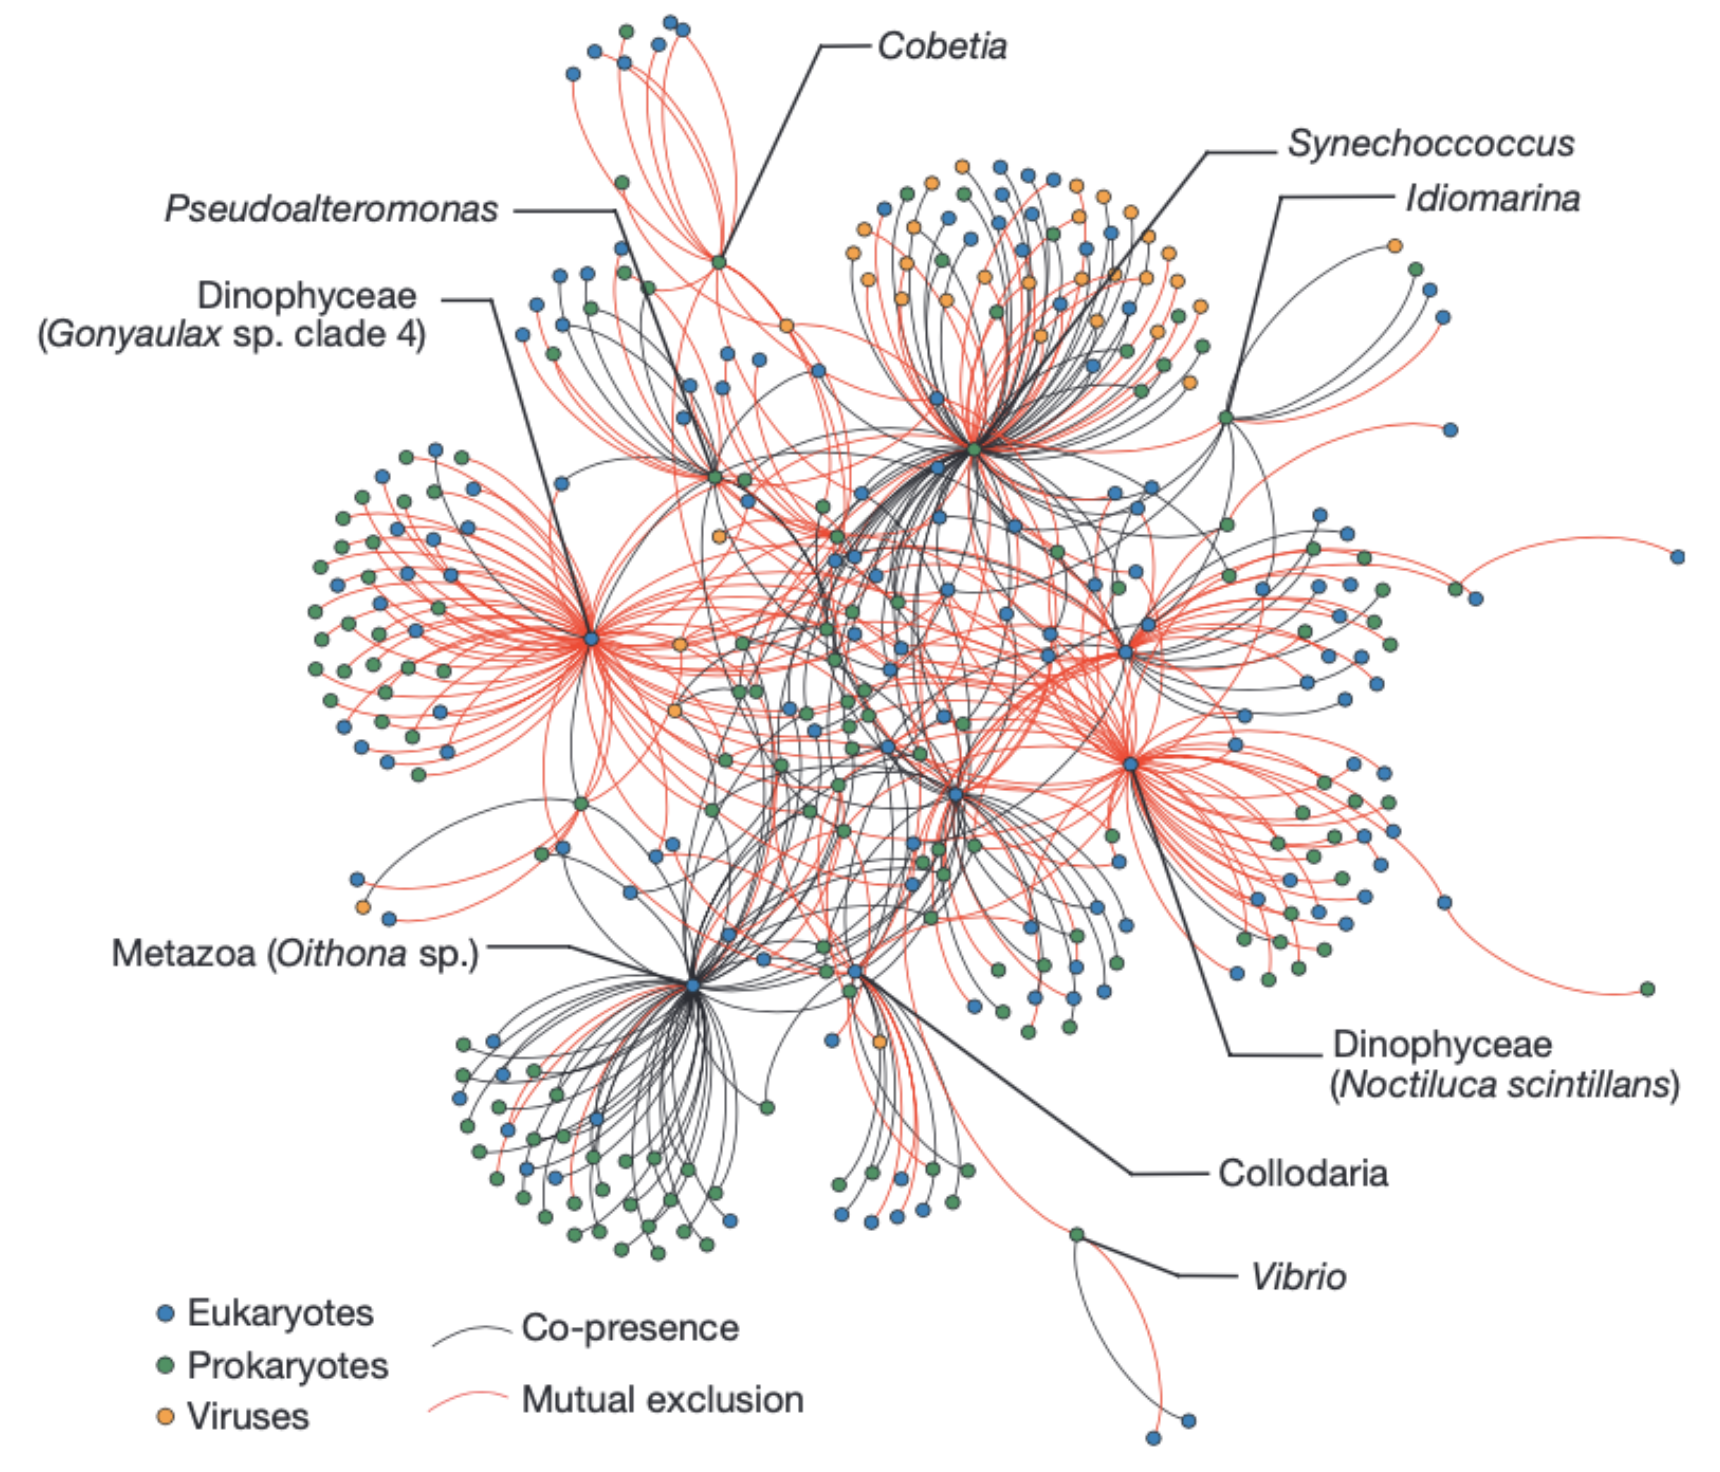
\includegraphics[width=0.7\linewidth]{figs/plancton.png}
\captionsetup{labelformat=empty}
\caption{Integrated plankton community network related to carbon export at 150m \citep{GCB16}.}
\label{PPI}
\end{figure}



This work is interested in species network inference, which is the art of identifying interactions from observed measures on a set of species. Network inference necessarily relies on a mathematical definition of species interactions, allowing to detect a broad range of interactions. Their biological meaning is unknown and would have to be identified by experts later on. 


A first idea of a mathematical species interaction is the correlation between the species abundances. However using correlation results in dense networks proving hard to analyze, as spurious edges appear between two variables correlated to the same third one \footnote{e.g. the number of covid 19 cases detected correlates with both the real number of cases and the number of tests done on the population, which induces a spurious correlation between the two latter where obviously there is no direct effect of one on the other.}.  Instead, using conditional dependence relationships between species provides with  a clear separation between direct and indirect effects, and therefore yields sparse and easy to interpret networks.


Graphical models are the dedicated mathematical framework for the modeling and inference of such networks, for they graphically represent a multivariate random variable conditional dependencies. Gaussian Graphical Models (GGM) in particular present with specific theoretical and algebraic properties which facilitate the inference. GGM  have been widely used on continuous data. \\

However measures on species are often counts, as is usually the case in ecology and in experiments using high-throughput sequencing technologies in genomics and microbiology. A way to go for network inference from count data with a distinction between direct and indirect effects is then to adopt a modeling for the count allowing the use of the GGM framework. To obtain interpretable results, the model should also account for measured experimental offsets and covariates. Furthermore, the observed measures on species are also very likely to be incomplete as it is difficult to know in advance all the factors governing a phenomenon. This causes the species interaction network to present spurious edges between the species which should be linked to the unobserved actor (species or covariate). A partial observation of the data thus provides with a marginal network instead of the complete one, leading to biased further interpretations and analyzes.\\


\section*{Objectives and outline} 
The aim of the present work is to develop a methodology for the network inference from incomplete abundance data. This task was divided into two sub-objectives. 
First, develop a method for network inference from abundance data. To this aim we model counts  using the Poisson log-normal distribution, taking advantage of the estimation procedure developed by \citet{CMR18}. This specific distribution includes a latent layer of Gaussian parameters, within which the inference of the species interaction network is performed. Following \citet{MeilaJaak} and \citet{SR17}, the inference is carried out using tree averaging, allowing for a complete and efficient exploration of the space of spanning tree graphs, and yielding edges probabilities.

Then, this work includes missing actors in the model to account for incomplete data. There we model the missing actors as additional latent variables of the model Gaussian latent layer. The Gaussian graphical model parameters maximum likelihood estimators detailed in \citet{Lau96} are adapted to the specific case of spanning tree structures, and applied within a variational Expectation Maximization algorithm.

  \subsection*{Chapter 1}
The first chapter covers in details the mathematical and technical background used in Chapters 2 and 3. It defines the general framework of graphical models and its link with conditional independence relationships. The particular properties of the Gaussian graphical models are then presented, along with its maximum likelihood estimators. Two network inference methods are detailed: the penalized regularization which estimates the precision matrix in a sparse manner, and tree averaging which efficiently explores the super-exponential space of spanning-tree structures. This chapter then draws a state of the art of the strategies for the modelization of multivariate counts.

   \subsection*{Chapter 2}
   Chapter 2 details the proposed methodology for the inference of species interaction networks from measures of joint abundances. Counts are modeled in a hierarchical manner: a spanning-tree graph $T$ is first drawn, then parameters $\Zbf$ are modeled  conditionally on $T$ as a multivariate Gaussian faithful to $T$, and finally counts $\Ybf$ follow a Poisson log-normal distribution with parameters $\Zbf$. This model thus involves two latent layers of parameters: $\Zbf$ and $T$, and can be described by the following graph:
 
 \begin{center}
	\begin{tikzpicture}	
      \tikzstyle{every edge}=[-,>=stealth',auto,thin,draw]
		\node (A1) at (0*\length, 0*\length) {$T$};
		\node (A2) at (1*\length, 0*\length) {$\Zbf$};
		\node (A3) at (2*\length, 0*\length) {$\Ybf$};
		\draw (A1) edge [->](A2);
        \draw (A2) edge [->] (A3);
	\end{tikzpicture} 
   \end{center}
 
The model inference estimates the tree distribution using an EM algorithm, which had not been done before. The proposed methodology is implemented in the R package EMtree (\url{github.com/Rmomal/EMtree}). It is compared to state-of-the-art approaches and applied to two empirical datasets from ecology and microbiology. This chapter has been published in the journal \textit{Methods in Ecology and Evolution} \citep{MRA20}. The presented appendices are extended with a vignette showing usage examples of the EMtree package.

    \subsection*{Chapter 3}
This chapter presents an extended version of the previous model developed in Chapter 2 to include possible missing actors. The Gaussian latent layer is assumed to involve additional unobserved variables. The Gaussian layer is considered in its normalized form and denoted $\Ubf$.  This model thus involves three latent layers: $T$, $\Ubf_O$ where "O" stands for "observed", and $\Ubf_H$ where "H" stands for "hidden", and can be described by the following graph:
 
 \begin{center}
	\begin{tikzpicture}	
      \tikzstyle{every edge}=[-,>=stealth',auto,thin,draw]
		\node (A1) at (0.625*\length, 2*\length) {$T$};
		\node (A2) at (0*\length, 1*\length) {$\Ubf_O$};
		\node (A3) at (1.25*\length, 1*\length) {$\Ubf_H   $};
		\node (A4) at (0*\length, 0*\length) {$\Ybf$};
		\draw (A1) edge [->](A2);
        \draw (A1) edge [->] (A3);
        \draw (A2) edge  (A3);
        \draw (A2) edge [->](A4);
	\end{tikzpicture} 
	  \end{center}
 
 The model is estimated with a variational EM algorithm, which takes advantage of the average on trees to use the adaptation to the context of spanning trees of the maximum likelihood estimators of GGM parameters detailed in \citet{Lau96}. The developed procedure is implemented in the R package nestor (\url{github.com/Rmomal/nestor}) and illustrated on two  empirical datasets from ecology. \\

This chapter has been submitted for publication in a statistical journal. The submitted supplementary material is enriched with a vignette showing usage examples of nestor, a section presenting different initialization methods and finally a comparison of nestor, EMtree and  PLN-network which is another method building on the PLN distribution but uses a penalized approach for the network inference.

  \subsection*{Chapter 4}
This final chapter introduces some perspectives of this work. After summarizing  the specifics of the developed methodology and discussing unresolved issues, natural extensions of the model are presented. They first include extensions about measures on the inferred network, with a method for estimating the latent layer precision matrix,  and a strategy  to use tree distributions for comparing networks. Then perspectives about the data at hand are discussed, namely how to handle other data types or datasets presenting with spatial dependencies. Finally a model for the network inference not resorting to a latent layer is presented. %using only discrete distributions is presented.
\newpage
 \section*{Notations}
 
 \begin{description}
 \item[Operations:]  \begin{itemize}
     \item[]
 \item[] $|\cdot|$ : matrix determinant
 \item[] $\odot$ : Hadamard product
 \end{itemize}
 \item[Matrices:] \begin{itemize}
     \item[]
 \item[] $\Ybf$ : observed counts
 \item[] $\Zbf$ :  latent Gaussian parameters 
 \item[] $\Ubf$ :  latent normalized Gaussian parameters 
 \item[] $\Xbf$ : covariates 
 \item[] $O$ :  measured offsets
 \end{itemize}
 \item[Dimensions:]\begin{itemize}
     \item[]
 \item[] $n$ : samples
 \item[] $p$ : observed species
 \item[] $r$ : unobserved actors
 \item[] $d$ : covariates
 \end{itemize}
 \end{description} 
\clearemptydoublepage
\ActivateBG 
\chapter{Mathematical Framework}
 
\vspace{1cm}
This first chapter  details the technical background extracted from the literature which is used in the next chapters. It begins by covering all the required notions of graphical models, with a  focus on the spanning tree structures specifics. Then we present Gaussian graphical models properties and explain why it is a golden framework for network inference. After a reminder on the Expectation-Maximization algorithm as well as its variational interpretation, the last part is a state of the art of network inference from abundance data and presents methods stemming from both genomics and ecology. This chapter is meant to be independent from the rest of this work, and therefore repetitions with published work is unavoidable.


 \section{Graphical Models}
 A graphical model is classically described as a probabilistic model which conditional dependence structure is given by a graph. This first section gives the general framework of graphical models, definitions and properties are adapted from \citet{Lau96}.  Then the special case of  spanning tree graphs is presented.
 %%%%%%%%%%%%%%%%%%%%%%%%%%
 \subsection{General framework}
 A graph is defined as a pair $\G=(V,E)$ such that $V$ is a finite set of vertices, and the set of edges $E$ is a subset of $V\times V$ such that vertices are not linked to themselves and there are no multiple edges between two vertices. For any given pair of nodes $(k,\ell)$, we denote an edge by $k\sim\ell$ and an absence of edge by $k\nsim \ell$. In the literature, $V$ can be composed of both quantitative and qualitative variables. However here we  only use variables of one kind (quantitative) and so $V$ is called pure. The following definitions apply to the particular case of a pure vertex set $V$ and an undirected graph $\G$.\\

Let's first consider a subset $A$ of the vertex set $V$. $A$ is said to be \textit{complete} if all the nodes it contains are linked with each other. If $A$ is additionally of maximal size, it is then called a \textit{clique}. This definition makes the expression "maximal clique" a pleonasm. The \textit{subgraph} $\G_A$ defined by $A$  is obtained from $\G$ by keeping edges with both endpoints in $A$. Furthermore if $A$, $B$ and $S$ are disjoint subsets of $V$, $S$ is said to \textit{separate} $A$ from $B$ if any path from $\G_A$ to $\G_B$ intersects with $\G_S$. The following notions of decomposable graphs and perfect sequences are central in the definition of a graphical model.
 
 \begin{definition}[Proper decomposition]
 A triple $(A, B, C)$ of disjoint subsets of the pure vertex set $V$ of an undirected graph $\G$ form a decomposition of $\G$ if $V=A\cup B \cup C$, and if $C$ satisfies:
 \begin{enumerate}[label=(\roman*)]
 \item $C$ is a complete subset of  $V$,
 \item $C$ separates $A$ from $B$.
 \end{enumerate}
 If $A$ and $B$ are both non-empty, the decomposition is proper.
 \end{definition}
 
 Therefore a decomposition is simply a separation of the set of nodes on complete subsets. This allows to recursively define a decomposable graph:
 \begin{definition}[Decomposable graph]
 An undirected graph is decomposable if it is complete, or if there exists a proper decomposition $(A, B, C)$ into decomposable subgraphs $\G_{A\cup B}$ and $\G_{B\cup C}$.
 \end{definition}
 This definition proves to be very useful in demonstrations of decomposable graphs properties, but not to prove that a graph is decomposable. The following notion of triangulation will help.
 
 \begin{definition}[Triangulated graph]
 An undirected graph $\G$ is said to be triangulated if loops in $\G$ connect three nodes at most.
 \end{definition} 
 In other words in a triangulated graph, the loop of maximal size will form a triangle. Triangulated graphs are also called chordal graphs. Then, a \textit{sequence} is a numbered list of subsets of the node set. A sequence is called \textit{perfect} under the following conditions on the subsets and the numbering order:
 \begin{definition}[Perfect sequence]\label{def:seq}
 Let $B_1,...,B_k$ be a sequence of subsets of the pure set of vertex $V$ of the undirected graph $\G$. Let $H_j=B_1\cup .. \cup B_j$, and $S_j = H_{j-1} \cap B_j$. The sequence is perfect if it satisfies the following conditions:
 \begin{enumerate}[label=(\roman*)]
 \item for all $i>1$ there is a $j<i$ such that $S_i \subseteq B_j$ (running intersection property),
 \item each $S_i$ is a complete subset.
 \end{enumerate}
 $H_j$ are called the histories and $S_j$ the separators.
 \end{definition}
% \begin{definition}[perfect numbering]
% A perfect numbering of the vertices $V$ of $\G$ is a numbering $\alpha_1,...,\alpha_k$ such that the sequence $B_1,...,B_k$ with 
% $$B_j = cl(\alpha_j) \cap \{\alpha_1,...,\alpha_j\}, j\geq 1 $$ is a perfect sequence. This implies that each $B_j$ is a complete subset.
% \end{definition}
 An example where separators are complete but the sequence is not perfect is the following.
\begin{figure}[H]
 \begin{center}
	\begin{tikzpicture}	
      \tikzstyle{every edge}=[-,>=stealth',shorten >=1pt,auto,thin,draw]
		\node[basic, label=above:1] (A1) at (-1*\edgeunit,0*\edgeunit) {};
		\node[basic, label=below:2] (A2) at (0,0) {};
		\node[basic, label=below:3] (A3) at (1*\edgeunit,0*\edgeunit) {};
		\node[basic, label=above:4] (A4) at (2*\edgeunit,0) {};
		\node[basic, label=right:5] (A5) at (0.5*\edgeunit,0.8*\edgeunit) {};
		\path (A1) edge  (A2)
        (A2) edge [] (A3)
        (A3) edge [] (A4)
        (A2) edge [] (A5)
        (A5) edge [] (A3);
	\end{tikzpicture} 
 \caption{An undirected graph with 5 nodes.}
  \label{ex:graph1}
    \end{center}
\end{figure}
Consider the graph in Figure \ref{ex:graph1}. A sequence is $B=\big\{B_1=\{1,2\}, B_2=\{3,4\},B_3=\{2,3,5\}\big\}$, with the separators $S_2=\varnothing, S_3=\{2,3\}$. As $\{2,3\}$ is not a subset of any of the $B_i$ with $i$ less than 3, the running intersection property is violated and $B$ is not perfect. Inverting $B_2$ and $B_3$ however yields a perfect sequence. 
%Note that in the definition the empty set can be included in the set of separators, but an easy way to find a perfect sequence is simply to avoid this situation. 
The notion of perfect sequence allows to define the multiplicity of a separator:
 \begin{definition}[multiplicity of a separator]
 The multiplicity $\nu (S)$ of the separator $S$ is an index counting the number of times $S$ occurs in a perfect sequence.
 \end{definition}
 
\begin{figure}[H]
 \begin{center}
	\begin{tikzpicture}	
      \tikzstyle{every edge}=[-,>=stealth',shorten >=1pt,auto,thin,draw]
		\node[basic, label=left:1] (A1) at (-0.2*\edgeunit,-0.7*\edgeunit) {};
		\node[basic, label=left:2] (A2) at (-0.4,0) {};
		\node[basic, label=left:3] (A3) at (-0.2*\edgeunit,0.7*\edgeunit) {};
		\node[basic, label=above:4] (A4) at (1*\edgeunit,0) {};
		\node[basic, label=right:5] (A5) at (1.6*\edgeunit,1.2*\edgeunit) {};
		\node[basic, label=right:6] (A6) at (2.3*\edgeunit,0.7) {};
		\node[basic, label=right:7] (A7) at (2.4*\edgeunit,0*\edgeunit) {};
		\node[basic, label=right:8] (A8) at (1.5*\edgeunit,-0.8*\edgeunit) {};
		\path (A1) edge  (A2)
        (A2) edge [] (A4)
        (A4) edge [] (A1)
        (A2) edge [] (A3)
        (A4) edge [] (A3)
        (A4) edge [] (A5)
        (A4) edge [] (A6)
        (A5) edge [] (A6)
        (A7) edge [] (A6)
        (A4) edge [] (A7)
        (A4) edge [] (A8);
	\end{tikzpicture} 
 \caption{An undirected decomposable graph with 8 nodes.}
  \label{ex:graph}
    \end{center}
\end{figure}
 Let's consider the graph of Figure \ref{ex:graph}. A perfect sequence of its cliques is 
$C_1=\{1,2,4\}$, $C_2=\{2,3,4\}$, $C_3=\{4,5,6\}$, $C_4=\{4,6,7\}$, $C_5=\{4,8\}$. The corresponding separators are $S_2=\{2,4\}$, $S_3=S_5=\{4\}$, $S_4=\{4,6\},$ which gives the following multiplicities: $\nu(\{2,4\})=1$,  $\nu(\{4,6\})=1$, $\nu(\{4\})=2$.  


\begin{prop}
\label{decomp}
The following conditions are equivalent for an undirected graph $\G$:
\begin{enumerate}[label=(\roman*)]
\item $\G$ is decomposable.
\item The cliques of $\G$ can form a perfect sequence.
\item $\G$ is triangulated.
\end{enumerate}
\end{prop}

 This property is the most useful in practice, as it states that as soon as a graph does not present with cycles of size 4 or more, it is decomposable on its cliques. This decomposition is essential to the graphical model properties, as we will see in Gaussian graphical models.
 
 %%%%%%%%%%%%%%%%%%%%%%%%%%
\subsection{Characterization of conditional independence}
The notion of conditional independence is central in the theory of graphical models. All that follows focuses on the case of variables associated with positive and continuous densities. Let's consider three random variables $X,Y$ and $Z$ with joint distribution $f$. The conditional independence of $X$ and $Y$ conditional on $Z$ is linked to the factorization of $f$. More precisely: 
$$X \independent Y \mid Z \iff f(x,y,z) = f(x,z) \, f(y,z)/f(z). $$
Conditional independence can be understood in terms of information. That is, "$X$ is independent of $Y$, given $Z$" means that knowing $Z$, $Y$ will not bring any new information on $X$, and conversely. The Markov property below is the link between conditional independence of variables and its representation in an undirected graph. Let's consider a collection of random variables $(X_v)_{v\in V}$ taking values in probability spaces $(\mathcal{X}_v)_{v\in V}$, and $\mathcal{X}=\otimes_{v\in V} \mathcal{X}_v$. We further denote for any subset $A$ of $V$, $X_A=(X_v)_{v\in A}$, and $\G$ a graph with vertex set $V$. 

\begin{definition}[Markov property]\label{def:markov}
A probability measure P on $\mathcal{X}$ is \textit{global} Markov relative to the undirected graph $\G$ if for any triple $(A, B, S)$ of disjoint subset of $V$ such that:
 $$ \text{S separates A from B } \Rightarrow X_A\independent X_B \mid X_S$$
 If additionally $X_A\independent X_B \mid X_S \Rightarrow \text{S separates A from B}  $, then P is \textit{faithful} Markov and $\G$ perfectly describes the conditional dependence structure of P.
\end{definition}
Therefore if a distribution is only global Markov, its related graph is possibly too dense: it can contain edges between variables which are actually conditionally independent from one another. 
\begin{definition}[Factorization]\label{def:fact}
A probability measure P on $\mathcal{X}$ factorizes according to $\G$ if it has density $f$ with respect to measure $\mu = \otimes_{v\in V} \mu_v$, where $f$ can be written as
$$f(x) = \prod_{c\in \mathcal{C} }\psi_c(x),$$
where $\mathcal{C}$ denotes the set of cliques of $\G$, and for any subset $C$ of the vertex set $V$, $\psi_C$ is a positive function of $X_C$ only.
\end{definition}
The following theorem links definitions \ref{def:markov} and \ref{def:fact} for positive and continuous distributions:

\begin{theorem}[Hammersley and Clifford] \label{thm:ham}
For any undirected graph $\G$ and probability distribution P with positive and continuous density $f$ with respect to a product measure $\mu$, it holds that:
$$P\text{ factorizes according to } \G \iff P\text{ is global Markov relative to }\G $$
\end{theorem}

This equivalence means in practice that writing a density in a product form on some combinations of its variable helps identify conditional independence relations.

%%%%%%%%%%%%%%%%%%%%%%%%%%
 \subsection{Spanning trees}
Trees are graphs with no cycles, meaning that all cliques are edges only. When a tree connects all the nodes, it is called a spanning tree. This particular type of graph is both the sparsest connected graph, and the most connected graph without loops. This feature makes it a decomposable graph by definition, following condition $(iii)$ of Proposition \ref{decomp}.  The following result is obtained directly.

\begin{prop}
If $T$ is a spanning tree, all of its separators are nodes. For any node $k$ of $T$ we denote $d(k)$ its degree. Then its multiplicity in any perfect sequence is $\nu(k) = d(k)-1$.
\end{prop}
 
 
 The study of the spanning tree structure began in the latter part of the $19^{th}$ century. Then, Arthur Cayley established that the total number of spanning trees of a complete graph with $p$ nodes is $p^{p-2}$. Kirchhoff generalized this result in a theorem known as the "all-minor" theorem, using the notion of graph Laplacian matrix.
  \begin{definition}[Laplacian matrix]
 \label{laplacian}
 The Laplacian matrix $\Qbf$ of a symmetric matrix $\Wbf=[w_{jk} ]_{1\leq j,k\leq p}$ is as follows :

\[
 [\Qbf]_{jk}  =\begin{cases}
    -w_{jk}  & 1\leq j<k \leq p\\
    \sum_{u=1}^p w_{ju} & 1\leq j=k \leq p.
    \end{cases}
\]
When $\Wbf$ is a graph adjacency matrix, $\Qbf$ is called the graph Laplacian matrix and its diagonal is composed of the degrees of each node.
 \end{definition}
 
 Hereafter we denote $\Abf^{uv}$ the squared matrix $\Abf$ deprived from its $u$th row and $v$th column, and remind that the $(u, v)$-minor of $\Abf$ is the determinant of this deprived matrix, namely $|\Abf^{uv}|$.
 
 \begin{theorem}[Kirchhoff's theorem]\label{th:kir}
 For any graph $\G$, let  $\Qb_\G$ denote its graph Laplacian matrix. Then for any  pair of nodes $\{u,v\}$, the total number of spanning trees in $\G$ is equal to  $|\Qb_\G^{uv}|$.
\end{theorem}  

 
The total number of spanning trees in any graph can thus be computed in polynomial time. Theorem \ref{th:kir} was extended for weighted graphs in the late 20th century as follows, where $\mathcal{T}$ denotes the spanning tree space on $V=\{1,...,p\}$:

\begin{theorem}[Matrix Tree Theorem  \cite{matrixtree,MeilaJaak}] \label{thmm:MTT}
    For any symmetric weight matrix $\Wbf$ with all entries in $\mathds{R}^+$, the sum over all spanning trees of the product of the weights of their edges is equal to any minor of its Laplacian $\Qbf$. That is, for any $1 \leq u, v \leq p$,
 
   \[
    W := \sum_{T\in\mathcal{T}} \prod_{(j, k)\in T} w_{jk} = |\Qbf^{uv}|.
    \]
   
\end{theorem}    

Consequently, the operation of summing over all spanning trees can be carried out in a computationally efficient way. \cite{MeilaJaak}  build on this result to provide a close form expression for the derivative of the sum-product $W$ with respect to each entry of the input weight matrix $\Wbf$.   Without loss of generality, we choose $\Qbf^{11}$.

\begin{lemma} [\cite{MeilaJaak}] \label{lemm:Meila}
    Define the entries of the symmetric matrix $\Mbf$ as
\[    
 [\Mbf]_{jk} =\begin{cases}
    \left[(\Qbf^{11})^{-1}\right]_{jj} + \left[(\Qbf^{11})^{-1}\right]_{kk} -2\left[(\Qbf^{11})^{-1}\right]_{jk} & 1< j<k \leq p\\
    \left[(\Qbf^{11})^{-1}\right]_{jj} & k=1, 1< j \leq p  \\
    0 &  j=k .
    \end{cases}
\] 
it then holds that
$$\partial_{w_{jk}} W = [\Mbf]_{jk}  \times W.$$
\end{lemma}

Theorem \ref{thmm:MTT} actually gives the solution to the computation of the sum on trees of a product function on the edges of a spanning tree, which can be judiciously used combined with  Lemma \ref{lemm:Meila} to perform network inference using average on trees, as we will see later on. 

%%%%%%%%%%%%%%%%%%%%%%%%%%
%%%%%%%%%%%%%%%%%%%%%%%%%%
 \section{Gaussian Graphical Models}
 Gaussian graphical models (GGM) describe the conditional dependency structure of a  multivariate Gaussian distribution. The different properties of the multivariate Gaussian distribution allow some specific interpretation and estimation results of its related graphical model,  making the GGM a sound and very clever framework to work with.
 
 %%%%%%%%%%%%%%%%%%%%%%%%%%
 \subsection{Specific properties}
The multivariate Gaussian distribution possesses various properties which facilitate computations as well as interpretations. Two in particular are of interest in the graphical models setting. The first one concerns the natural handy writing of its density.
 \begin{prop}\label{pp:ggm1}
 Let $X\sim \mathcal{N}(\mu, \Sigmab)$ with precision matrix $\Omegab=\Sigmab^{-1}$ and $X_k$ denote the $k^{th}$ column of $X$. Then the associated density $f$ factorizes as:
 $$f(X) \propto \prod_{k,\ell, \omega_{kl}\neq 0} \exp(-X_{k}\omega_{k\ell}X_{\ell}/2)$$
 \end{prop}
 Therefore as the density naturally factorizes, Theorem \ref{thm:ham} states that $f$ is global Markov relative to an undirected graph $\G$, the edges of which are determined by the non-null entries of its precision matrix $\Omegab$.  The multivariate Gaussian distribution also presents with a facilitating property about conditional independence, reminded below.
 
 \begin{prop}\label{pp:ggm2}If  $X\sim \mathcal{N}_V(\mu, \Omegab^{-1})$, then it holds for any $k,\ell\in V$ with $k\neq \ell$ that
$$X_k \independent X_\ell \mid X_{V\setminus\{k,\ell\}} \iff \omega_{k\ell}=0 $$
 \end{prop}
  Proposition \ref{pp:ggm2} is not a consequence of proposition \ref{pp:ggm1}, and comes directly from the fact that the $2\times 2$  covariance matrix of variables $k$ and $l$ conditional on all others expresses in terms of the precision matrix : $$\Sigmab_{k,l\mid V\setminus\{k,l\}} = |\Omegab_{\{k,l\}}|^{-1} \left(\begin{array}{cc}
\omega_{kk} & -\omega_{kl}\\
-\omega_{kl} & \omega_{ll}  
  \end{array}\right).$$
Combining the above propositions \ref{pp:ggm1} and \ref{pp:ggm2}, it is easy to see that a conditional independence implies a null entry in $\Omegab$, which in turn implies no edge between the corresponding nodes in $\G$. This proves the following result.

\begin{prop}[Faithfulness property]\label{ggm:faith}
 Let $X\sim \mathcal{N}(\mu, \Omegab^{-1})$ with associated density $f$, $\G$ the graph which edges represent the non-nul entries of $\Omega$. Then $f$ is faithful Markov relative to $\G$,  and it holds that:
 $$k\nsim \ell \iff  X_k \independent X_\ell \mid X_{V\setminus\{k,\ell\}} \iff \omega_{k\ell}=0.$$
\end{prop} 

Proposition \ref{ggm:faith} is key for estimation in the GGM framework, as it states that finding the null precision entries gives all the graph. The Gaussian framework also offers specific conditioning results, and in particular the regression interpretation of $\Omegab$ entries.

\begin{prop}[Regression interpretation]\label{ggm:reg}
 Considering $X\sim \mathcal{N}(\mu, \Omegab^{-1})$, the linear regression of  $X_j$ on $X_{\setminus j}$ writes :
$$X_j = \sum_{k\neq j} \beta_{jk} X_k + \varepsilon_j,\qquad \text{where}\qquad\varepsilon_j \sim \Ncal (0, \omega_{jj}^{-1}), \qquad \beta_{jk} = \frac{\omega_{jk}}{\omega_{jj}}.$$

\end{prop}
Hence $\omega_{jk}$ is, up to a scalar, the coefficient of $X_k$ in the multiple regression of $X_j$ on all other variables. This result is at the basis GGM inference methods relying on regression, which we will see later on. But first, let's turn to Lauritzen's  parameters estimation for GGM, made possible by the faithfulness property.

%%%%%%%%%%%%%%%%%%%%%%%%%%
 \subsection{Maximum likelihood estimation}
In this section we adopt the following notations: for any  squared  matrix $\Abf$ of dimension $p$ and $B$ a subset of $V=\{1,...,p\}$, we let $\Abf_B$ refer to the bloc $B$ of $\Abf$: $\Abf_{B}=(a_{ij})_{\{i,j\}\in B}$.   $[\Abf_B]^p$ then denotes the matrix obtained by filling up with zero entries to obtain full dimension $p\times p$, so that:
$$([\Abf_B]^p )_{ij}=\left\{ \begin{array}{rl}
a_{ij} & \text{if } \{i,j\}\in B\\
0 &  \text{if } \{i,j\}\in V_{\setminus B}
\end{array}\right.$$

Hereafter we consider  $X\sim\Ncal (\mu, \Omegab)$ with dimension $p$. If $X$ is associated with a decomposable graph $\G$, the Markov property \ref{def:markov} decomposes accordingly and reflects in a multiplicative property for the density, and additive property for the concentration matrix. More precisely, considering a perfect sequence of the cliques of $\G$ as in Definition \ref{def:seq}, we have that
 $$f(X)=\dfrac{\prod_{C\in \mathcal{C}} f(X_C)}{\prod_{S\in \mathcal{S}} f(X_S)^{\nu(S)}}.$$
This general expression of the density across decomposition of the graph is very helpful in likelihood computations, especially when some hypotheses are made on the structure of $\G$. The following lemma gives the expressions for $\Omegab$ and its determinant:
 \begin{lemma} In a decomposable Gaussian graphical model with precision matrix $\Omegab = \Sigmab^{-1}$ of dimension $p$:
 \begin{equation*}
 \left\{
 \begin{array}{rl}
 \Omegab &= \sum_{C\in \mathcal{C}} \big[(\Sigmab_C)^{-1}\big]^p - \sum_{S\in \mathcal{S}} \nu(S)  \big[(\Sigmab_S)^{-1}\big]^p \\\\
 |\Omegab| &=\dfrac{\prod_{C\in \mathcal{C}} |\Sigmab_C|^{-1}}{\prod_{S\in \mathcal{S}} |\Sigmab_S|^{-\nu(S)}}
 \end{array} \right.
\end{equation*}  
where $\mathcal{C}$ is the set of cliques of $\G$ and $\mathcal{S}$ the set of separators with multiplicities $\nu$ in any perfect sequence. 
\end{lemma}

The GGM framework allows exact results for the estimation of maximum likelihood estimators (MLE) of the mean vector, the precision matrix, its determinant and the terms of the covariance matrix corresponding to edges in the graph. They all depend on the sufficient statistic that is the sum of squared deviations, defined as follows where $X^i$ denotes the $i^{th}$ sample of $X$:
\begin{definition}
Denoting $\xbar{X}$ the empirical mean of the multivariate Gaussian $X$, the sum of squared deviations matrix, also known as total sum of squares,  is given by:
$$SSD = \sum_{i=1}^n (X^i - \xbar{X})(X^i - \xbar{X})^\intercal = X^\intercal X - n  \xbar{X} \,\xbar{X}^\intercal.$$
\end{definition}
The following theorems \ref{mle:sig} and \ref{mle:ome} give the MLE estimators in the GGM framework using $SSD=(ssd_{ij})_{ij}$.
 
\begin{theorem}[\citet{Lau96} Theorem 5.3]\label{mle:sig}
In the Gaussian graphical model,  the MLE of the unknown mean and covariance matrix exist with probability one if $n>p$. When they exist, the estimate of the mean is $\widehat{\mu} = \xbar{X}$, and the estimate of the unknown covariance matrix $\Sigmab$ is determined as the unique solution of the system of equations
\begin{equation*}
 \left\{
 \begin{array}{rl}
 n\widehat{\sigma}_{jj} = ssd_{jj}&, j\in V\\
 n\widehat{\sigma}_{k\ell} = ssd_{k\ell}&, k\sim\ell, (k,\ell) \in V
 \end{array} \right.
\end{equation*}  
which also satisfies the model restriction $\omega_{k\ell} =0 \iff k\nsim \ell $.
\end{theorem}

\begin{theorem}[\citet{Lau96} Proposition 5.9]\label{mle:ome}
In a Gaussian graphical model with graph $\G$, the MLE of the precision matrix exists with probability one if $n>max_{C\in\mathcal{C}}|C|$. It is then given as
$$\widehat{\Omegab} = n \bigg\{\sum_{C\in\mathcal{C}} \big[(SSD_C)^{-1}\big]^p-\sum_{S\in\mathcal{S}} \nu(S) \big[(SSD_S)^{-1}\big]^p\bigg\},$$
where $\mathcal{C}$ is the set of cliques of $\G$ and $\mathcal{S}$ the set of separators with multiplicities $\nu$ in any perfect sequence. The determinant of the estimate can be calculated as
$$|\widehat{\Omegab}| = n^p \dfrac{\prod_{C\in\mathcal{C}}|(SSD_C)^{-1}|}{\prod_{S\in\mathcal{S}} (|(SSD_S)^{-1}|)^{\nu(S)}}$$
\end{theorem}
 
The stronger condition $n>p$ of Theorem \ref{mle:sig} is only sufficient, whereas the condition $n>max_{C\in\mathcal{C}}|C|$ of Theorem \ref{mle:ome} is necessary for the existence of all the MLE, as it ensures the positive definiteness of all $SSD_C$ (otherwise some might not have full rank).  

 All of the above maximum likelihood estimators require the precise knowledge of the graph structure and is therefore rarely available. However relying on simple structures (e.g. spanning trees) greatly simplifies the expressions and make their use possible.

%%%%%%%%%%%%%%%%%%%%%%%%%%
\subsection{Network inference from Gaussian data}
  Network inference here refers to the inference of the conditional dependence structure of multiple variables jointly observed in a series of sites. The interactions between the species are unknown, therefore this is not to be confused with the art of inferring a network parameters (e.g. sign and strength of the interactions) from observations of repeated interactions.
  
In the special framework of GGM, conditional dependence relations are perfectly represented by the non-nul entries of the precision matrix $\Omegab$, as specified in Proposition \ref{ggm:faith}. The general approach to network inference in GGM is then to perform a sparse estimation of $\Omegab$.

 \subsubsection{Penalized estimation}
 In a standard linear regression model, penalized estimation is used to select predictors. The most popular penalized method is the Lasso \citep{lasso} which apply the $\ell_1$ penalty and estimates the $\beta$ coefficients as the solution of:
 $$\argmin_{\beta \in \mathds{R}^p} \big\{ ||\Yb - \Xb\beta ||^2_2 + \lambda ||\beta||_1\big\}, \qquad ||\beta||_=\sum_{i=1}^p |\beta_i|,$$
 where $\lambda$ is a penalty called the regularization parameter.  The form of the $\ell_1$ penalty forces some coefficients to exactly equal zero.
 \textcolor{red}{use with the regression interpretation of networks}.
 
 Penalized estimation in GGM is performed by the Graphical Lasso (glasso) \citep{glasso}, which introduces sparsity in the precision matrix by imposing Lasso penalties on its entries. The log-likelihood of a GGM writes:
 $$L_\lambda(\Omegab) = \log |\Omegab| +\tr{\Yb^\intercal \Yb \Omegab}+cst .$$
 The precision matrix is then estimated as the matrix which maximizes the penalized log-likelihood:
 $$\argmax_{\Omegab\geq 0} \big\{L_\lambda(\Omegab) - \lambda ||\Omegab||_1\big\}, \qquad ||\Omegab||_1 = \sum_{j\neq k} |\omega_{jk}|.$$
The glasso gives a sparse penalized maximum likelihood estimator of $\Omegab$, and select the network edges by forcing some of them to zero in the precision matrix. The greater the penalty $\lambda$, the less edges are included in the network and therefore choosing $\lambda$ is critical for the glasso. The selection of $\lambda$ can be performed using classical tools such as cross-validation, Akaike information criterion (AIC),  Bayesian information criterion (BIC) or its extended version.  Another popular approach is to perform a stability selection with StARS \citep{stars}, which aims the network robustness under random sampling.

 %builds on the regression interpretation of the partial correlation

 
 \subsubsection{Averaging on trees}
  Another way to foster sparsity in the graph is to assume a sparse structure. Spanning trees are the sparsest connected graphs, and it is possible to computes the tree which maximizes the likelihood from observations using  the Chow-Liu algorithm \citep{ChowLiu}. However the data conditional dependency structure is unlikely to be a tree in general, and tree averages provide the opportunity to take advantage of all the spanning trees properties while being flexible on the data structure. \\

 The idea behind using an average on spanning trees to perform network inference  is that the underlying graphical model is supposed to be random and is itself treated as a latent parameter of the model. This graph is also supposed to be a tree and to follow a distribution which is decomposable on its edges as in the definition below.
\begin{definition}[decomposable tree distribution]
For any symmetric weight matrix $\Wbf$ with all positive entries, we denote $W$ the sum-product form defined in Theorem \ref{thmm:MTT} A decomposable  distribution for the tree $T$ is then defined as follows:
$$p_{\Wbf}(T) = \prod_{k,\ell \in T} w_{k\ell} / W ,$$
so that the probability of a tree is proportional to the product of its edges weights.
\end{definition}

An interesting property of a decomposable tree distribution is that it is stable under a multiplicative transformation applied to its weight matrix. This is particularly useful during the implementation.

Once a probability is assigned to each tree of the spanning tree space, the probability of an edge in a tree can be defined as the sum of the probabilities of trees containing this edge. Namely for the tree $T$:
$$\mathds{P}\{kl\in T\} = \sum_{T\in \mathcal{T}} p_{\Wbf}(T).$$
The following lemma  states that it is possible to compute all edges probabilities at the same time, and this at the cost of the inversion of the  Laplacian matrix of the edges weights.

\begin{lemma} [\cite{kirshner}] \label{lem:Kirshner}
    Let $p_{\Wbf}$ be a decomposable tree distribution with symmetric and positive weight matrix $\Wbf$. Taking the symmetric matrix $\Mbf$ as defined in Lemma  \ref{lemm:Meila}, the probability for an edge $kl$ to be in the tree $T$ writes:
 
$$\mathds{P}\{kl\in T\} =  w_{kl}\: \Mbf_{kl}$$
\end{lemma}

The final output of a strategy using an average on trees is not the latent tree presenting with the highest probability, but the matrix filled with the edges probabilities obtained by summing on all trees. Therefore the output is a weighted network which has no reasons to be shaped as a tree itself.

%%%%%%%%%%%%%%%%%%%%%%%%%%%%%%%%%%
%%%%%%%%%%%%%%%%%%%%%%%%%%%%%%%%%%
\section{Inference of incomplete data models}
Incomplete data can refer either to unobserved variables due to experimental constraints, or latent variables in the model. The Expectation-Maximization (EM) algorithm \citep{DLR77} is the classic approach to compute the maximum likelihood estimate in presence of hidden variables. In this section we present the general principles of the EM algorithm, as well as its variational version. We let $\Ybf$ denote the observed incomplete data, $\Zbf$ the hidden variables, $p$ their joint distribution with parameter vector $\thetab$.
 
%%%%%%%%%%%%%%%%%%%%%%%%%%
 \subsection{Expectation-Maximization algorithm}
 The EM algorithm is an iterative procedure which maximizes the expected value on  the complete log-likelihood $\log p_\thetab (\Ybf, \Zbf)$ conditional on the observed data $Y$. The iteration $t+1$ consists in two steps:
 \begin{description}
 \item [E step:] estimate $\Esp_{\thetab^t}[\log p_\thetab (\Ybf, \Zbf)\mid \Ybf]$
 \item [M step:] $\thetab^{t+1} = \argmax_\thetab \{ \Esp_{\thetab^t}[\log p_\thetab (\Ybf, \Zbf)\mid \Ybf]\}$
 \end{description} 
 The  log-likelihood $\log p_{thetab} (\Ybf)$ increases with the iterations of the EM algorithm \citep{DLR77}. \\
 
 
 Another formulation of the EM assumes a distribution $q$ for the hidden variables \citep{NH98} and defines a  lower bound $\bound$ as:
 $$\bound(\thetabf, q) = \log p_\thetab (\Ybf) - KL(q(\Zbf) || p_\thetab(\Zbf\mid\Ybf)),$$
 where $KL(p||q) = -\Esp_q[\log q - log p]$ is the Küllback-Leibler divergence. In this formulation, the link between the maximization of $\bound$ and that of the likelihood is made clear. The iteration $t+1$ of the EM can then be written as a double maximization :
  \begin{description}
 \item [E step:]  $q^{t+1}=\argmax_q \{ \bound(\thetabf^t, q^t)\}$
 \item [M step:] $\thetab^{t+1} = \argmax_\thetab \{ \bound(\thetabf^t, q^{t+1})\}$
 \end{description} 
 
In the E step, the search space for $q^{t+1}$ is the whole set of distributions on the definition space of the hidden variables. The solution is the distribution which cancels the Küllback-Leibler divergence, and that is $p_\thetab(\Zbf\mid\Ybf)$. Unfortunately the latter is not always available, in which case one might resort to a variational computation.
 

%%%%%%%%%%%%%%%%%%%%%%%%%% 
 \subsection{Variational estimation}
 When $p_\thetab(\Zbf\mid\Ybf)$ cannot be computed, the variational version of the EM reduces the search space of the $q$ distribution to a set $Q$, which is chosen to ease the computations of the M step. Doing so results in a variational approximation of $p_\thetab(\Zbf\mid\Ybf)$. Therefore in a  Variation EM (VEM) algorithm, the E step is replaced by a VE step, which is  
 $$q^{t+1}=\argmax_{q\in Q} \{ \bound(\thetabf^t, q^t)\}.$$
 
 A widely used choice for $Q$ are product-form distributions, such that for $K$ hidden variables $Q=\{q(\Zbf)=\prod_{k=1}^K q_k(z_k)\}$. This set of distribution results in a so-called a mean-field approximation. \\
 
In the variational bayesian setting, \citet{beal} derive update equations  for the hidden variables as well as the parameters. Random parameters are a specificity of the bayesian framework, and in fact they can be viewed as other hidden variables. Hidden entities in proposition \ref{beal} below can thus be latent factors, unobserved variables, or bayesian parameters.

 \begin{prop}[\citet{beal}]\label{beal}
 Let's consider a variational EM with observed data $\Ybf$ and $K$ hidden variables $\Zbf=\{z_1,...,z_K\}$. If the approximation is mean-field, then at step $t+1$ and for any $k$ in $\{1,...,p\}$ the update of the variational marginal distribution $q_k$ in the VE step is:
$$ q_k^{(t+1)}(z_k)  \propto \exp \left\{ \Esp_{q_{\setminus k}^t} \left[ \log p_{\thetabf^{t+1}}(\Ybf, \Zbf) \right] \right\}.$$
\end{prop}


 
%%%%%%%%%%%%%%%%%%%%%%%%%%%%%%%%%%
%%%%%%%%%%%%%%%%%%%%%%%%%%%%%%%%%%
\section{Network inference from count data}
  Inferring a network directly from count data would require to jointly model abundances with a multivariate discrete distribution. Unfortunately such distribution is not available, and the majority of techniques transposes the problem in the Gaussian framework, enabling to take advantage of the multivariate Gaussian distribution easy-handling and convenient properties.
  
  \subsection{Joint species distribution models}
Joint species distribution models (JSDM) are a general class of statistical parametric models for multiple discrete variables, for example the abundances of multiple species. JSDMs are an extension of the generalized linear model and thus readily handle covariates and offsets. Additionally they capture the correlation between the variables, and resorts to Gaussian random effects and a link function to do so. Hereafter we consider the input abundance data $\Yb$, and denote by the index $i$ the rows (samples) and the index $j$ the columns (species) of $\Yb$. A multivariate random effect $\zb_i$ is introduced to each data sample $\yb_i$.  Denoting $\xb_i$ the vector of covariates with regression coefficients $\thetab_j$, $o_{ij}$ a possible offset  and $g(\cdot)$ a link function, the mean abundance $m_{ij}$  in a JSDM can be specified in a general manner as follows:
$$g(m_{ij}) = o_{ij}+\xb_i^\intercal  \thetab_j + z_{ij}, \qquad \zb_i \sim \Ncal(0, \Sigmab).$$

The art of JSDMs then resides in the specification of $g$ and the random effects. The following section presents some of the most used settings in ecology and genomics.

\subsection{Shift to Gaussian universe} 
\subsubsection{Transformations}
The first idea when it comes to transposing counts into the Gaussian framework is to transform them. Doing so allows to analyze the data without resorting to discrete modeling. A common transformation of counts is to apply the log function, with a  small constant $c$ added to counts to avoid zeros (pseudo-counts). In this case the mean abundance is simply modeled as $\log(m_{ij}+c)$ and assumed to follow a multivariate Gaussian distribution. 

In genomics, high throughput sequencing yields  samples $\yb_i$  of observed counts of $p$ species or taxa that are constrained by the library size $\kappa_i$, a technical parameter of the experiment, such that $\sum_j y_{ij}=\kappa_i$ \citep{GMP17}. Thus the available observations are not absolute counts but relative counts, and each sample can be viewed as a compositional vector \citep{A82} sampled from the simplex
$$\mathcal{S}_i^p = \bigg\{ \boldsymbol{u}=(u_1,...,u_p)\in \mathds{R}^p\bigg\rvert\sum_{i=1}^p u_i = \kappa_i\bigg\}.$$
The transposed compositional representation is to consider  genes counts across all samples and to represent the relative gene expression per site, namely for gene $j$ and sample $i$: $\frac{y_{ij}}{\sum_i y_{ij}}$. Inputs are then the expression profiles of each gene \citep{RMR18}, onto which transformations  can be applied. 
There exists several transformations for compositional data to change the $\kappa_i$-sum constraint, the most popular being the centered log-ratio transformation  which writes:
$$clr(\yb)=\left(\log \frac{y_1}{m(\yb)}, ..., \log \frac{y_p}{m(\yb)}\right), $$
where $m(\cdot)$ is the geometric mean. A clr-transformed vector is constrained to a zero sum. In the framework of joint modeling, the clr function can be used as a link function to account for covariates and offsets. Recent works on network inference use the clr transformation  \citep{kurtz}, or the logistic normal distribution \citep{AS80} to model relative counts \citep{gcoda}.


\subsubsection{Copulas}
Copulas are  joint  distributions which map the marginal  cumulative distribution functions of a multivariate random vector.  They are used to describe the dependence between random variables, and in particular for Gaussian copulas the correlation matrix can be estimated. In their original form, they only apply to continuous marginals, and their extension to discrete data has been controversial \citep{F17}. However recent developments made the use of  Gaussian copula coupled with discrete marginal distributions possible \citep{PCJ12,PHW18}, opening the way to the application of copulas in the analysis of multivariate count data \citep{AVP19}. In this context, a first step estimates each $p$ marginal univariate discrete distributions parameters while accounting for covariates and possible offsets. Then the distribution of the response Gaussian copula is computed as a $p-$dimensional integrand (see \citet{PHW18}). \citet{PWT19} proved that  Gaussian copulas are a relevant and promising approach to the problem of network inference from abundance data, even if the computation cost remains substantial as it requires importance sampling as well as Monte Carlo expectation maximization algorithms. One way of taking advantage of the copula theory without having to actually estimate the joint distribution is to use copulas as a data transformation.\cite{MRFcov} resort to the nonparanormal transformation of counts which is a semiparametric Gaussian copula \citep{LLW09}, in an attempt to estimate network parameters varying across a gradient of covariates. 

\subsubsection{Latent variables}

Latent variables enable the modeling of multivariate discrete data using a hierarchical setting where random discrete variables are modeled conditionally to random latent variables.  Two specifications of  latent variables stand out in community ecology \citep{WBO15}:  the Multivariate Generalized Linear Mixed Model (GLMM) \citep{OHS10, PTM14}, and the Latent Variable Model (LVM)  \citep{OAP16, OTN17}. The difference between these models lies in the dimension of their respective random effects: there are as many latent variables as there are species in the GLMM, whereas in the LVM their number is a parameter of the model. 

In more details, in a LVM the random effect associated to the mean abundance $m_{ij}$ is a linear combination of a set of latent variables, and is generally specified as:
 $$g(m_{ij}) = o_{ij}+\xb_i^\intercal  \thetab_j +\sum_{k=1}^K z_{ik} \lambda_{kj},$$
 where $K$ is the number of latent factors included in the model, and the matrix $\Lambdab$ gathers the factors loadings $\lambdab_j$ in columns. Abundances are then assumed to follow
 \begin{align*}
 y_{ij}\mid \zb_i &\sim F(m_{ij}, \phi_j)\\
\zb_i&\sim \Ncal(0, \boldsymbol{I}),
 \end{align*}
and the covariance matrix of the latent layer of random effects can be computed from the factor loadings as $\Sigmab=\Lambdab^\intercal \Lambdab$.\\

In the case of a GLMM, $K=p$ and latent variables and abundances are  modeled as:
 \begin{align*}
 y_{ij}\mid \zb_i &\sim F(m_{ij}, \phi_j)\\
 \zb_i &\sim \Ncal(0, \Sigmab),
 \end{align*} 
 where $F$ is a distribution with mean $m_{ij}$ and dispersion parameter $\phi_j$. The Poisson log-normal distribution (PLN, \citet{AiH89}), estimated in \citet{CMR18} and used in \citet{MRA20}, is a GLMM where $F$ is the Poisson distribution and $g$ the exponential function.  
 
 \subsection{Network inference}
 \textcolor{red}{!Not final !}\\
 Network inference from count data generally moves the problem in the Gaussian framework  in order to  take advantage of all the aforementioned results on Gaussian graphical models. \\
 
 
\begin{table}[H]
\begin{tabular}{l|ccc|cc|cc|}
\cline{2-8}
 & \multicolumn{3}{c|}{ Gaussian shift} & \multicolumn{2}{c|}{Network inference} & \multicolumn{2}{c|}{Estimation} \\ \cline{2-8} 
 & Trans. & LV & Copulas & Penalized & Trees & MCMC & EM \\ \hline
\multicolumn{1}{|l|}{gCoda} & x &  &  & x &  &  &  \\ \hline
\multicolumn{1}{|l|}{ecoCopula} &  &  & x & x &  & x &  \\ \hline
\multicolumn{1}{|l|}{(V)EMtree} &  & x &  &  & x &  & x \\ \hline
\multicolumn{1}{|l|}{MInt} &  & x &  & x &  &  &  \\ \hline
\multicolumn{1}{|l|}{MRFcov} &  &  & x & x &  &  &  \\ \hline
\multicolumn{1}{|l|}{SpiecEasi} & x &  &  & x &  &  &  \\ \hline
\multicolumn{1}{|l|}{LITree} & \multicolumn{1}{l}{\cellcolor[HTML]{d8d8d8}} & \multicolumn{1}{l}{\cellcolor[HTML]{d8d8d8}} & \multicolumn{1}{l|}{\cellcolor[HTML]{d8d8d8}} & \multicolumn{1}{l}{} & \multicolumn{1}{c|}{x} & \multicolumn{1}{l}{} & \multicolumn{1}{c|}{x} \\ \hline
\multicolumn{1}{|l|}{saturnin} & \multicolumn{1}{l}{\cellcolor[HTML]{d8d8d8}} & \multicolumn{1}{l}{\cellcolor[HTML]{d8d8d8}} & \multicolumn{1}{l|}{\cellcolor[HTML]{d8d8d8}} & \multicolumn{1}{l}{} & \multicolumn{1}{c|}{x} & \multicolumn{1}{c}{x} & \multicolumn{1}{l|}{} \\ \hline

\end{tabular}
\end{table}
 %%%%%%%%%%%%%%%%%%%%%%%%%%%%%%%%%%
%%%%%%%%%%%%%%%%%%%%%%%%%%%%%%%%%%

  
 
\chapter{Network Inference from Abundance Data}
%chap 2
\section{Model}
	PLN, VEM et EM
	\section{Data simulation}
modèle PLN ou pas, problème de connaître la structure latente

	\section{Comparison to existing methods in ecology}
	\subsection{Methods }
	
	détail comportement des méthodes, leurs spécificités
	
	\subsection{performance in network inference}
	\subsection{performance in edge ranking}
	\subsection{performance in interaction strength reconstruction}
	
 
\chapter{Inference with Missing Actor}

%chap3

 % intro
%Les réseaux :
%- [ ] C’est quoi
%- [ ] À quoi ça sert (les enjeux, appliqué)
%- [ ] Quelles sont les questions qui se posent (que dit la recherche)
%
%- [ ] Lauritzen pour les nuls
%
%L’inférence de réseaux :
%- [ ] Quelle méthode pour quel réseau
%- [ ] Auxquelles on se compare, pourquoi elles sont comme ça comment elles marchent et ce qui manque

  \section*{Biological context}
 \subsection*{Networks}
 A network is an intuitive object which anyone can easily relate to. It is first of all a graphical tool representing the links between different entities. This helps understand how a system organizes and have a direct image of it. It is also an analysis tool which can unravel sensible information about the system, its structure and the different roles in its organization. Networks are versatile tools that are  used in many domains (e.g. sociology, linguistics, computer sciences, neurosciences, climatology, psychology, etc.) and can take various forms to adapt to each problem.  They can be directed or undirected. Some link entities with multiple kinds of edges (multidimensional), or have different layers (multiplex), others link groups of disconnected objects (multipartite). In biology, the most typical networks simply represent the species (nodes) and their relationships (edges).

Various types of species interactions are studied with networks. For example, their is a rich literature of networks for plant-pollinator and host-parasite relationships in ecology. These species interactions are clearly defined and directly observed in the field. Contacts of pollination or parasitism are counted and networks constructed from these interaction abundances.
\begin{figure}
\centering
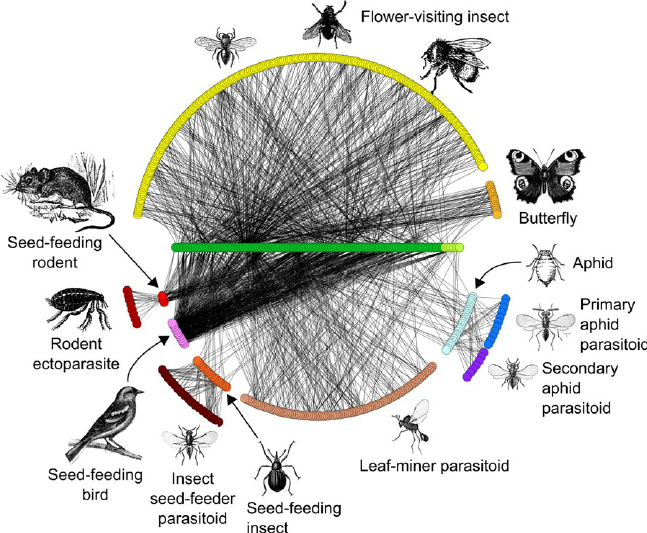
\includegraphics[width=0.7\linewidth]{figs/pocock.png}
\caption{Species interaction networks at Norwood Farm, Somerset, UK \citep{PED12,BRM13}.}
\label{pocock}
\end{figure}
 However many mechanisms cannot be observed and may not be well defined. One way to discover them may then be to resort to a more mathematical definition of species interactions. Working with the latter allows the study of community assembly mechanisms with the inference of networks representing guilds of species in community ecology. This type of network is extensively used in genomics for protein-protein interaction network, or gene regulatory networks, or in microbiology to study the output of a metabarcoding experiment assessing the composition of a microbiome. 
 
 \begin{figure}
\centering
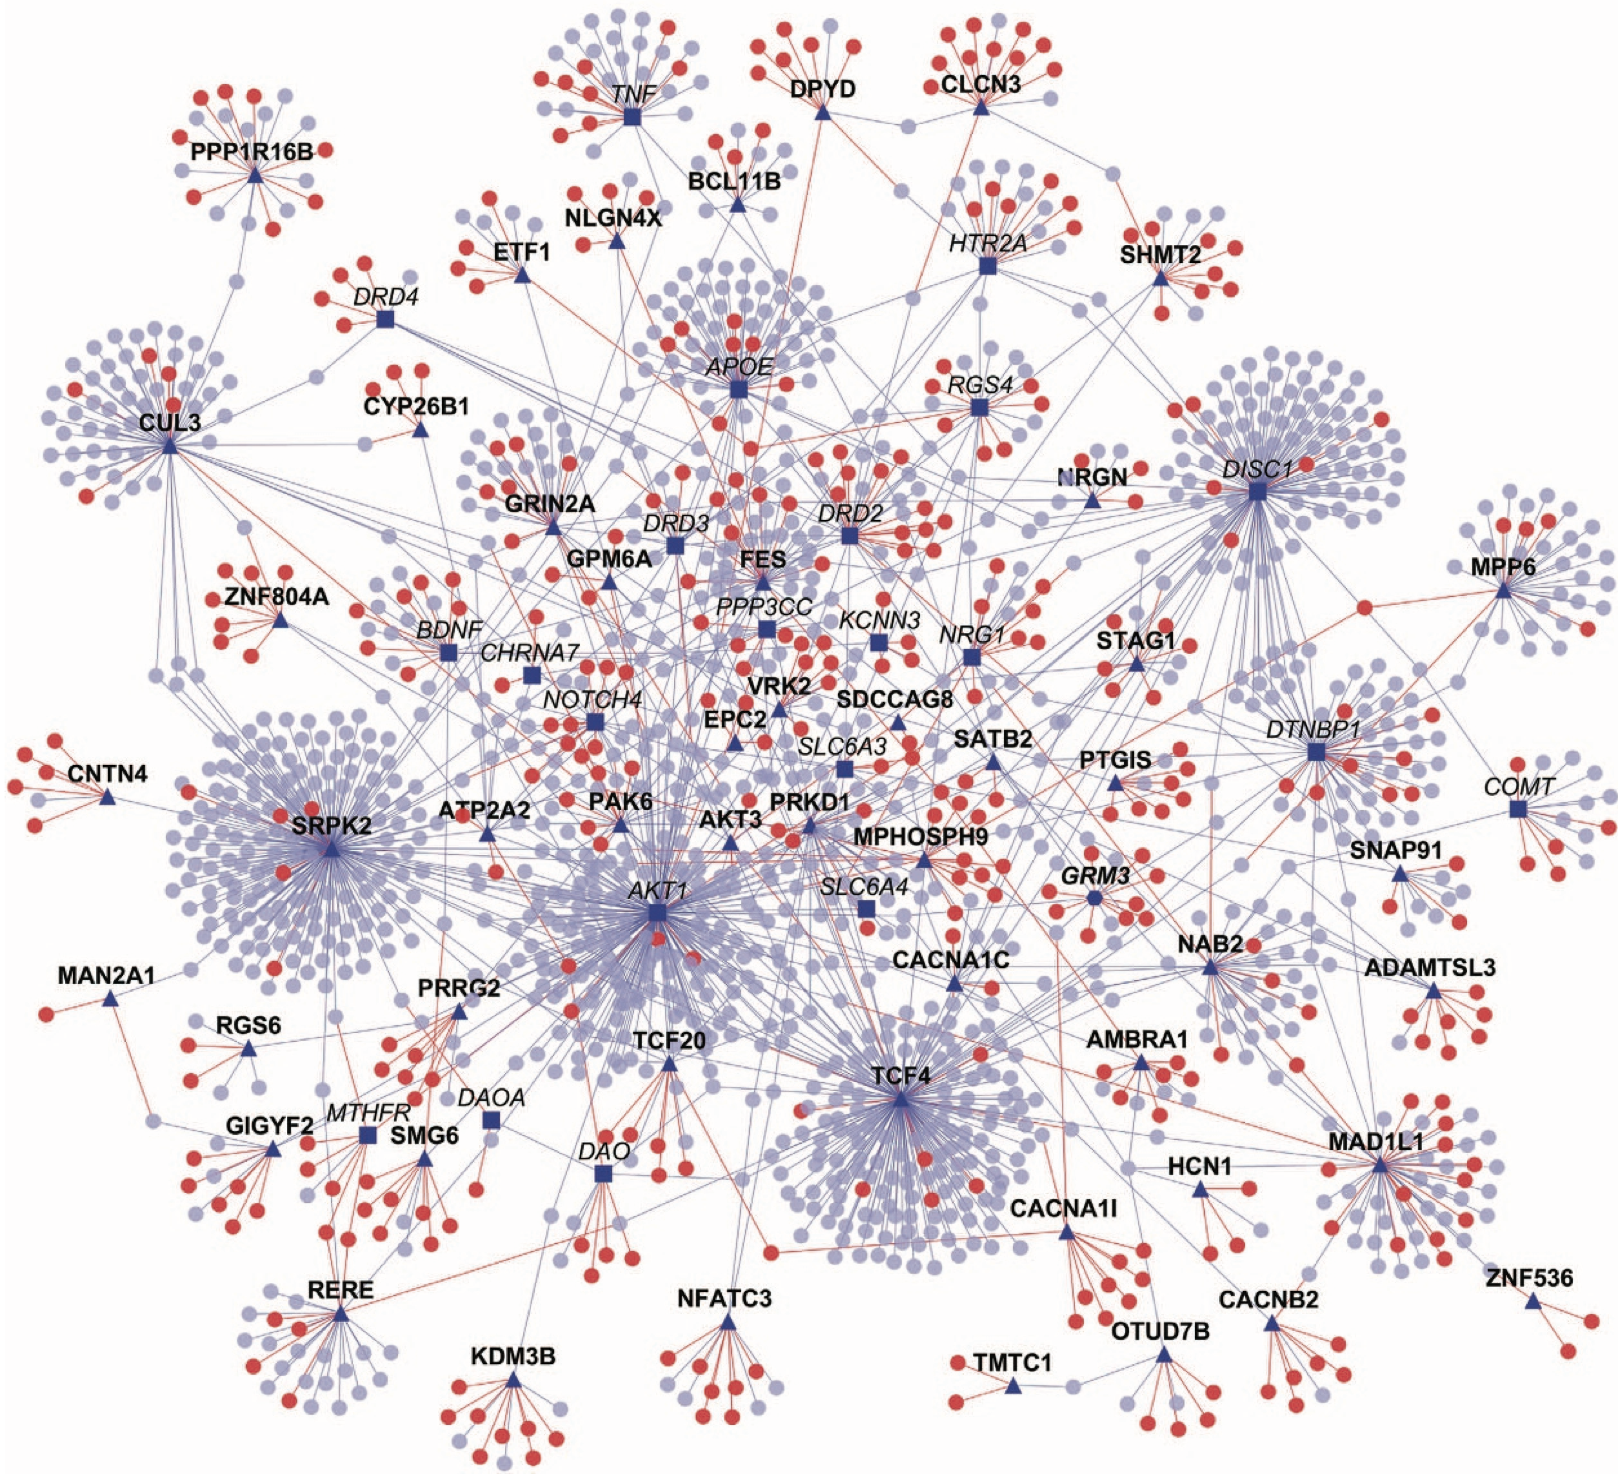
\includegraphics[width=0.7\linewidth]{figs/PPInetwork.png}
\caption{Protein-protein interactions between genes involved in schizophrenia \citep{GTH16}.}
\label{PPI}
\end{figure}

  \subsection*{Statistical interactions}
The correlations between the species measures first come to mind as a statistical characterization of an interaction. These are easily obtained, yet their corresponding networks are hard to interpret. Indeed, two covariates correlating with a same third one will appear correlated, even if they have no direct effect on each other\footnote{e.g. the number of covid 19 cases detected correlates with both the real number of cases and the number of tests done on the population, which induces a spurious correlation between the two latter where obviously there is no direct effect of one on the other.}. This phenomena of spurious correlations complicates both the analysis and the interpretation by inducing a very high number of edges  which cannot be categorized as direct or indirect associations between the species. 
 
 Conditional dependencies are then very useful measures of interaction. They describe dependencies between each pair of species conditional on all others. That is, all other species measures kept fixed, their measures should still be correlated. A link between two species can then be interpreted as a direct association. This yields a network of species conditional dependence (link) and independence (absence of link), which is interpretable and falls within the well-studied mathematical framework of graphical models.
 
 \subsection*{Measures on species}
 Networks of statistical interactions are obtained from datasets of repeated measures on a set of species, which can be of various types. Measures can be continuous, as for example the output of gene expression profiling experiments using DNA microarrays, which  are  fluorescences measures from targeted genes. Using a Gaussian approximation, these measures of genes expressions can be used to derive genes regulatory networks.  Measures can also be binary, as in co-occurrence data in ecology, which record the joint presences and absences of a set of species in several sites. \citet{CAM16}.
%développer les données de co-occurence

Abundance data  are joint counts of species in a series of sites (also known as assemblages data in ecology). Recent technologies made this type of data increasingly available. Assemblages data were rare in ecology as they implied intensive sampling efforts, which is now greatly facilitated by camera traps and sensors. In metagenomics, high-throughput sequencing technologies for metabarcoding experiments made it possible  to get joint counts of pseudo-species (operational taxonomic units (OTUs)) abundances.  Both domains work with the same type of output: a dataset of joint (pseudo-)species abundances from different sites or samples.\\
%développer les metabarcoding et OTU


Once the data has been collected, it is very likely that not all species or covariates were observed: there exists missing actors and data is incomplete. In the network, the existence of a missing actor translates into appearance of edges between all the species it should connect with, creating dense cliques of species which are not actually conditionally dependent on one another. A second objective of this work is to take missing actors into account during network inference in order to get more accurate interpretations.

\section*{Network inference}
% ce qui existe et motivation du sujet
\section*{Objectives}
 \subsection*{Graphical models and Trees}
The dedicated framework for the representation of conditional dependency structures are graphical models. Gaussian Graphical Models (GGM) in particular provide with appealing algebraic properties for network inference, which are detailed in \citet{Lau96}. Exploring the set of possible graphs is a non-ending task, and we chose to reduce the searching space to that of spanning trees. This is the sparsest connected structure, and enjoys specific algebraic properties allowing to sum on all possible spanning trees at the cost of a determinant calculus. Our network inference methodology relies on spanning trees and \citet{Lau96} maximum likelihood estimators for multivariate Gaussian graphical models.

%caser le missing actor qq part
 \subsection*{Modeling abundance data}
 As this ideal framework of GGM is not directly applicable to abundance data, there exist two possible ways to proceed: either apply a Gaussian transformation to the data, or rely on Gaussian latent vectors in the framework of Joint Species Distribution Models (JSDM). Our methodology resorts to the latter, and more specifically to the Poisson log-normal distribution to model the counts. This distribution allows easy handling of both covariates and offsets, as well as take overdispersion into account thanks to its Gaussian random parameters. 
 
 
 \subsection*{Estimation procedure} %or algorithm
The central model we adopt involves a Gaussian layer of parameters which is a mixture on all spanning trees. Each component of the mixture is a Gaussian distribution which dependency structure is a spanning tree. This represents two hidden layers of parameters, which we first estimates with an Estimation-Maximization (EM) algorithm. Then to infer missing actors of the network, we resort to a variational (VEM) approach.

\section*{Outline} 
  \subsection*{Chapter 1}
The first chapter details the mathematical tools and technical results for the statistical modeling and the network inference used in Chapters 2 and 3.

   \subsection*{Chapter 2}
   This chapter details a method to infer undirected networks representing conditional statistical dependencies between the species from their joint abundance measures.  The proposed methodology, implemented in the R package \texttt{EMtree},  is compared to state of the art approaches and applied to two empirical datasets from ecology and metagenomics. This chapter has been published as an article in the journal \textit{Methods in Ecology and Evolution} \citep{MRA20}.
   
    \subsection*{Chapter 3}
This chapter details a variational approach to the inference of a missing actor in the network. The reconstruction of missing actor(s) is implemented in the R package \texttt{nestor} and illustrated on two  empirical datasets from ecology. This chapter has been submitted for publication in the \textit{Journal of the Royal Statistical Society: series C (applied statistics)}.
 
  \subsection*{Chapter 4}
This final chapter introduces some natural perspectives of this work. After concluding on the specifics of the developed methodology, natural extension are presented, including network comparison. The inclusion of spatialized data is discussed, as well as the possibility of network inference directly from the observed counts.
 \section*{Notations}
 
 \begin{description}
 \item[Operations:]  \begin{itemize}
     \item[]
 \item[] $|\cdot|$ : matrix determinant
 \item[] $\odot$ : Hadamard product
 \end{itemize}
 \item[Variables:] \begin{itemize}
     \item[]
 \item[] $\Ybf$ :  matrix  of observed counts
 \item[] $\Zbf$ : matrix of latent Gaussian parameters 
 \item[] $\Ubf$ : matrix of latent normalized Gaussian parameters 
 \item[] $\Xbf$ : matrix of covariates 
 \item[] $O$ : matrix of measured offsets
 \end{itemize}
 \item[Dimensions:]\begin{itemize}
     \item[]
 \item[] $n$ : number of samples
 \item[] $p$: number of observed species
 \item[] $r$: number of unobserved species
 \item[] $d$: number of covariates
 \end{itemize}
 \end{description} 
 

Let us first describe the typical type of data we consider. We assume that $p$ species have been observed in $n$ sites. \validSR{The abundances are gathered in the $n \times p$ matrix $\Yb$. $Y_{ij}$ is the abundance of species $j$ in site $i$, and  $\Yb_i$ the abundance vector collected in site $i$ ($i$th row of $\Yb$).} We further assume that a vector of covariates $\xb_i$ \validSR{of size $d$} has been measured in each site $i$ and that all covariates are gathered in the $n \times d$ matrix $\Xb$. The sites are supposed to be independent.

Our aim is to decipher the dependency structure between the $p$ species, accounting for the effect of the environmental covariates encoded in $\Xb$. As explained above, ignoring environmental covariates is more than likely to result in spurious edges. 

\paragraph{Mixed model.}
To distinguish between covariates effects and species interactions, we consider a mixed model which states that each abundance $Y_{ij}$ has a (conditional) Poisson distribution
 
\begin{equation} \label{eq:pY.Z}
    Y_{ij} \sim \Pcal\left(\exp(\xb_i^\intercal \thetab_j + o_{ij} + Z_{ij})\right).
\end{equation}
 
In model (\ref{eq:pY.Z}), $o_{ij}$ is the sample- and species-specific offset which accounts for the sampling effort. $\thetab_j$ is the vector of fixed regression coefficients measuring the effect of each covariate on species $j$ abundance. The regression part is similar to a general linear model as used in niche modeling \citep[see e.g.][]{austin2007species}. 
\modif{$Z_{ij}$ is the random effect associated with species $j$ in site $i$. 
Importantly, the coordinates of the site-specific random vector $\Zb_i = (Z_{i1}, \dots Z_{ip})$ are not independant: the multivariate random term $\Zb_i$ precisely accounts for the interactions that are not due to environmental fluctuations. 
For each site $i$, a vector $\Zb_i$ is associated with the corresponding abundance vector $\Yb_i$.}
The distribution given in Eq.~\eqref{eq:pY.Z} is over-dispersed as the Poisson parameter is itself random, which suits ecological modeling of abundance data \citep{Eco_overdisp}.

\bigskip
We now describe the distribution of the latent vector $\Zb_i$. To this aim, we adopt a version of Kirshner's model \citep{kirshner}, which states that a spanning tree $T$ is first drawn with probability
 
\begin{equation} \label{eq:pT}
    p(T) = \prod_{(j, k) \in T} \beta_{jk} / B,
\end{equation}
 
where $(j, k) \in T$ means that the edge connecting species $j$ and $k$ is part of the tree $T$ and where $B$ is a normalizing constant. Each edge weight $\beta_{jk}$ controls the probability for the edge $(j, k)$ to be in the interaction network. \\
Then for each site $i$, a vector $\Zb_i$ is drawn independently with conditional Gaussian distribution $(\Zb_i \mid T) \sim \Ncal(0, \Sigma_T)$, where the subscript T means that the distribution of $\Zb_i$ is {faithful} to $T$. When $T$ is a spanning tree, this faithfulness simply means this distribution can be factorized on the nodes and edges of $T$ as follows \citep[see][]{kirshner}:
 
\begin{equation} \label{eq:pZfact}
p(\Zb_i \mid T) = \prod_{j=1}^p p(Z_{ij}|T) \prod_{(j, k) \in T} \psi_{jk}(\Zb_i),
\end{equation}
 
where $\psi_{jk}(\Zb_i)$ does not depend on $T$. This factorization means that each edge of $T$ corresponds to a species pair in direct interaction;  all other pairs are conditionally independent. Experiments are independent, and in the sequel we consider the product of all $p(\Zb_i)$ and use the simpler notation $\psi_{jk} = \prod_i \psi_{jk}(\Zb_i)$ instead.\\

According to Eq.~\eqref{eq:pT}, each $\Zb_i$ has a Gaussian distribution conditional on the tree $T$, so its marginal distribution is a mixture of Gaussians: $\Zb_i \sim \sum_{T \in\mathcal{T}} p(T) \Ncal(0, \Sigma_T)$, where $\mathcal{T}$ is the set of all spanning trees. As a consequence, the joint distribution of the $\Zb_i$ is modeled by a mixture of distributions with tree-shaped dependency structure. \\
Besides, for all trees including the edge $(j, k)$, the estimate of the covariance term between the coordinates $j$ and $k$ is the same \citep[see][]{Lau96,SRS19}. Hence, we may define a global covariance matrix $\Sigmab$, filled with covariances that are each common to spanning trees containing a same edge. Each $\Sigmab_T$ is then built by extracting from $\Sigmab$ the covariances corresponding to the edges of $T$.



%%%%%%%%%%%%%%%%%%%%%%%%%%%%%%%%%%%%%%%%%%%%%%%%%%%%%%%%%%%%%%%%%%%%%%%%%%%%%%%%
\section{Inference} \label{sec:Inference}
%%%%%%%%%%%%%%%%%%%%%%%%%%%%%%%%%%%%%%%%%%%%%%%%%%%%%%%%%%%%%%%%%%%%%%%%%%%%%%%%

As said in the introduction, we  resort to a variational EM algorithm to perform the inference due to the complex latent structure.

%%%%%%%%%%%%%%%%%%%%%%%%%%%%%%%%%%%%%%%%%%%%%%%%%%%%%%%%%%%%%%%%%%%%%%%%%%%%%%%%%%%%%%%
\subsection{Variational inference}
%%%%%%%%%%%%%%%%%%%%%%%%%%%%%%%%%%%%%%%%%%%%%%%%%%%%%%%%%%%%%%%%%%%%%%%%%%%%%%%%%%%%%%%

The log-likelihood of the so-called {\sl complete} data, that is $(\Ybf, \Ubf, T)$, writes
\begin{align*}
\log p_{\thetabf, \betabf, \Omega}(\Ybf, \Ubf, T) 
& = \log p_\betabf(T) + \log p_{\Omegabf}(\Ubf \mid T) + \log p_\thetabf(\Ybf \mid \Ubf).
\end{align*}
where $\Omegabf$ stands for the set of all tree-specific precision matrices: $\Omegabf = \{\Omegabf_T, T \in \Tcal_{p+r}\}$.
The conditional distributions of the latent variables $\Ubf$ and of the tree $T$ given the data $\Ybf$ are both intractable. Variational inference then aims at maximizing a lower bound of the log-likelihood of the observed data, which writes in our context as
\begin{align} \label{eq:lower-bound}
\Jcal(\thetabf, \betabf, \Omega; q)
& = \log p_{\thetabf, \betabf, \Omega}(\Ybf) 
- KL\left(q(\Ubf, T) \| p_{\thetabf, \betabf, \Omega}(\Ubf, T \mid \Ybf) \right) \\
& = \Esp_q \log p_{\thetabf, \betabf, \Omega}(\Ybf,\Ubf, T) + \Hcal(q(\Ubf, T)), \nonumber
\end{align}
where $q(\Ubf,T)$ stands for the approximate joint conditional distribution of the latent layer and of the tree: $q(\Ubf, T) \simeq p(\Ubf, T \mid \Ybf)$. 

%%%%%%%%%%%%%%%%%%%%%%%%%%%%%%%%%%%%%%%%%%%%%%%%%%%%%%%%%%%%%%%%%%%%%%%%%%%%%%%%%%%%%%%
\subsubsection*{Approximate distribution.}
The efficiency of variational inference mostly depends on the choice of $q(\Ubf, T)$, which is a balance between computational ease and adequation to the target distribution $p(\Ubf, T \mid \Ybf)$. We adopt here a classical product form for the approximate distribution: we impose to the latent variables $\Ubf$ and to the tree $T$ to be independent according to $q$ (whereas actually they are not conditional on the data), with respective marginals $h$ and $g$:
$$
q(\Ubf, T) =  h(\Ubf)g(T).
$$
Because the sites are independent, and without further assumption, the distribution $h$ is a product over all sites. Following \cite{CMR18} we approximate the conditional distribution of each latent vector $\Ubf_i$ with a Gaussian distribution, that is:
$$
h(\Ubf) = \prod_i \Ncal_{p+r}(\Ubf_i; \mbf_i, \Sbf_i).
$$
with all $\Sbf_i$ diagonal. We gather all the mean vectors $\mbf_i$ in the $n \times (p+r)$ matrix $\Mbf$ and pile up the diagonals of all the variance matrices $\Sbf_i$ in the $n \times (p+r)$ matrix denoted $\Sbf$.

%%%%%%%%%%%%%%%%%%%%%%%%%%%%%%%%%%%%%%%%%%%%%%%%%%%%%%%%%%%%%%%%%%%%%%%%%%%%%%%%%%%%%%%
\subsubsection*{Variational EM.}
The variational EM algorithm then consists in maximizing the lower bound $\Jcal$ defined in \eqref{eq:lower-bound} with respect to the parameters (M step), and to the approximate distributions (VE step), alternatively. 
\begin{description}
\item[M step:] At iteration $t+1$, given the current approximate distribution $q^t(\Ubf, T) = g^t(T) h^t(\Ubf)$, the M step consists in the update of the model parameters, solving 
\begin{align} \label{eq:Mstep}
\thetabf^{t+1} & = \arg\max_\thetabf \; \Esp_{h^t} \left[ \log p_\thetabf(\Ybf \mid \Ubf) \right], 
& \Omegabf^{t+1} & = \arg\max_\Omegabf \; \Esp_{q^t} \left[ \log p_{\Omegabf}(\Ubf \mid T) \right], \nonumber \\
\betabf^{t+1} & = \arg\max_\betabf \; \Esp_{g^t} \left[ \log p_\betabf(T) \right].
\end{align}
Observe that the matrix of edge weights $\betabf$ is considered here as a parameter to be estimated, as opposed to \cite{RAR19}, where it was kept fixed and supposed to be given.
%
\item[VE step:] Maximising $\Jcal$ with respect to (wrt) $q$ is equivalent to minimizing the K\"ullback-Leibler divergence between $q(\Ubf, T)$ and $p_{\thetabf, \betabf, \Omega}(\Ubf, T \mid \Ybf)$ that appears in \eqref{eq:lower-bound}. Because we adopted a product form for $q$, the solution of the VE step for both $g$ and $h$ is known to be a mean-field approximation \citep{WaJ08}. More specifically, maximising $\Jcal$ gives
\begin{align} \label{eq:VEstep-g}
g^{t+1}(T) 
& \propto \exp \left\{ \Esp_{h^t} \left[ \log p_{\thetabf^{t+1}, \betabf^{t+1}, \Omega^{t+1}}(\Ybf, \Ubf, T) \right] \right\} \nonumber \\
& \propto \exp \left\{ \log p_{\betabf^{t+1}}(T) + \Esp_{h^t} \left[ \log p_{\Omegabf^{t+1}}(\Ubf \mid T) \right] \right\},
\end{align}
and
\begin{align} \label{eq:VEstep-hH}
h^{t+1}(\Ubf) 
& \propto \exp \left\{ \Esp_{g^{t+1}} \left[ \log p_{\thetabf^{t+1}, \betabf^{t+1}, \Omega^{t+1}}(\Ybf, \Ubf, T) \right] \right\} \nonumber \\
& \propto \exp \left\{ \Esp_{g^{t+1}} \left[ \log p_{\Omegabf^{t+1}}(\Ubf \mid T) \right] + \log p_{\thetabf^{t+1}}(\Ybf \mid \Ubf) \right\}. 
\end{align}
\end{description}

Observing that $\log p_\betabf(T) + \log p_{\Omegabf}(\Ubf \mid T)$ can be written as a sum over all the edges present in $T$, we see that $g^{t+1}(T)$ has a product form. So, without any further assumption, we may parametrize $g(T)$ in the same way as $p_\betabf(T)$:
\begin{equation} \label{eq:g}
g(T) = \prod_{jk \in T} \betat_{jk} / \Bt
\qquad \text{where} \quad
\Bt = \sum_{T \in \Tcal_{p+r}} \prod_{jk \in T} \betat_{jk}.
\end{equation}
We gather the $\betat_{jk}$'s in the $(p+r) \times (p+r)$ matrix $\betabft$. The parameters $\betabft$, $\Mbf$ and $\Sbf$ are called the variational parameters, in the sense that it is equivalent to optimize $\Jcal$ wrt $(g, h)$ or wrt $(\betabft, \Mbf, \Sbf)$.

%%%%%%%%%%%%%%%%%%%%%%%%%%%%%%%%%%%%%%%%%%%%%%%%%%%%%%%%%%%%%%%%%%%%%%%%%%%%%%%%%%%%%%%
\subsection{Proposed algorithm}
\label{algo}
%%%%%%%%%%%%%%%%%%%%%%%%%%%%%%%%%%%%%%%%%%%%%%%%%%%%%%%%%%%%%%%%%%%%%%%%%%%%%%%%%%%%%%%

The model we consider is an extension of the PLN model, for which an efficient inference algorithm have been implemented in \url{PLNmodels}, an R package available on CRAN \citep{CMR18,CMR19}. 

\subsubsection*{Prior estimates of $\thetabf$, $\Mbf_O$ and $\Sbf_O$.}
To alleviate the computational burden of the inference, we take advantage of this available tool to get an estimate of the regression coefficient matrix $\widehat{\thetabf}$ and an approximation of the parameters  of the observed latent variable conditional distribution $h_O(\Ubf_O) \simeq p(\Ubf_O \mid \Ybf)$. These latter parameters are $\Mbf_O$ and $\Sbf_O$ (first $p$  columns of $\Mbf$ and $\Sbf$ respectively) and we denote $\Mbft_O$ and $\Sbft_O$ their approximation. The quantities $\widehat{\thetabf}$, $\Mbft_O$ and $\Sbft_O$ are kept fixed in the rest of the algorithm, so the VEM algorithm only deals with the remaining unknown quantities: the model parameters $\betabf$, $\Omegabf$, and the variational parameters $\betabft$, $\Mbf_H$, $\Sbf_H$. 
% \textcolor{red}{[on ne dit plus que c'est sous-optimal ? "optimal value for MO and SO" est un peu fort ?]}
As a consequence, the final estimates we get yield a lower value of the objective function $\Jcal$ as compared to  an optimisation wrt all model and variational parameters.

%%%%%%%%%%%%%%%%%%%%%%%%%%%%%%%%%%%%%%%%%%%%%%%%%%%%%%%%%%%%%%%%%%%%%%%%%%%%%%%
\subsubsection*{M step.} This step deals with the update of the  model parameters $\betabf$ and $\Omegabf_T$. Some of the calculations are tedious and postponed to Appendix \ref{app:comput}.

\paragraph{Edges weights $\betabf$:} 
As shown in Equation \eqref{eq:Mstep}, the maximization of $\mathcal{J}$ requires the computation of the derivative of $\Esp_{g^t} [\log p_{\betabf}(T)]$ wrt $\betabf$, which includes the derivative of the normalizing constant $B$. The latter can be computed via an extension of the Matrix Tree theorem \citep[see][Lemma \ref{lem:Meila} reminded in Appendix \ref{app:tools}]{MeilaJaak}. Setting the derivative of the expectation to 0 yields the following update (same as in \citet{MRA20} and detailed in appendix \ref{up:beta}):
$$
\beta^{t+1}_{kl} 
= \frac{P^t_{kl}}{ M(\betabf^t)_{kl}},
$$
where $M(\betabf)$ is defined in Lemma \ref{lem:Meila} and $P^t_{kl}$ is the probability that the edge $(k, l)$ belongs to the tree $T$ according to $g^t$:
$$
P^t_{kl} = \mathds{P}_{g^t}\{kl \in T\} 
= \sum_{\substack{T  \in \mathcal{T}: \\ T \ni kl}} g^t(T) 
= \frac{1}{\Bt^t} \sum_{\substack{T  \in \mathcal{T}: \\ T \ni kl}} \prod_{uv \in T} \betat^t_{uv}.
$$
$P^t_{kl}$ is computed using a result from \citet{kirshner} (reminded as Lemma \ref{lem:Kirshner} in appendix A). We now define the binary variable $I_{Tkl}$ which indicates the presence of the edge $kl$ in tree $T$, so $P_{kl}^t = \Esp_{g^t} [I_{Tkl}]$ and $I_T = [I_{Tkl}]_{1 \leq k, l \leq (p+r)}$ is the adjacency matrix of tree $T$.

\paragraph{Precision matrices $\Omegabf_T$:}
For a given dependency structure in the Gaussian Graphical model framework, \cite{Lau96} gives maximum likelihood estimates for the precision matrix. 
These estimators are given as functions of sufficient statistics of the multivariate Gaussian distribution. Indeed in the exponential family framework, the M step of any EM algorithm requires the computation of the expectation of a sufficient statistic, under the current fit of the variational laws (see \citet{mclachlan}). Here as $\Ubf \mid T$ is centered, a sufficient statistic is $\Ubf^\intercal \Ubf$. We now let $SSD$ denote the matrix defined as 
$$
SSD^t = \Esp_{h^t} (\Ubf^\intercal \Ubf) = (\Mbf^t)^\intercal \Mbf^t + \Sbf^t_+,
$$
where $\Sbf^t_+ = \sum_i \Sbf^t_i$. Applying Lauritzen's formulas, we get:
%As $g^t$ is a discrete law on the space of spanning trees, maximizing each component of an expectation wrt $g$ amounts to  maximizing the whole expectation, meaning that maximizing for each tree $T$ will maximize $\mathcal{J}(\Ybf ; g,h)$.
%The off-diagonal and diagonal terms of $\hat{\Omega}_T$ write as follows with normalized data:
\begin{align} \label{omegaT}
\omega^{t+1}_{Tkl} & = \left\{
\begin{array}{ll}
\dfrac{ -ssd_{kl}^{\,t}/n}{1-(ssd_{kl}^{\,t}/n)^2} & \text{if } kl \in T \\
0 & \text{otherwise}
\end{array} 
\right., \\
\omega^{t+1}_{Tkk} & = 1 + \sum_l I_{Tkl} \dfrac{(ssd_{kl}^{\,t}/n)^2}{1-(ssd_{kl}^{\,t}/n)^2},
\nonumber
\end{align}
where $ssd^t_{kl}$ stands for the entry $kl$ of the matrix $SSD^t$.
The calculations are postponed to Appendix \ref{up:omega}. Observe that estimates of the off-diagonal entries $\omega^{t+1}_{Tkl}$ do not depend on $T$ provided that the edge $(k, l)$ belongs to $T$.  Thus the estimates of the off-diagonal terms of the precision matrices $\Omegabf_T$ are common to all trees sharing a given edge. This does not result from any assumption on the shape of  $\Omegabf_T$, but from the properties of the maximum likelihood estimate of Gaussian variance matrix. In the sequel we will simply denote off-diagonal terms by $\omega_{kl}$ (as opposed to $\omega_{Tkk}$ which still depends on $T$).\\

Other quantities are needed for later computations. Lauritzen  gives the maximum likelihood estimator of every entry of the correlation matrix $\Rbf_T$ corresponding to an edge $kl$ being part of $T$, which is
$ \Rbf_{Tkl}^{t+1} = ssd_{kl}^{\,t}/n. $
Hereafter for any matrix $A$, $A_{[kl]}$ refers to the bloc $kl$ of $A$: $A_{[kl]}=(a_{ij})_{\{i,j\}\in\{k,l\}}$. The determinant of $\Omegabf^{t+1}_T$ factorizes on the edges of $T$ and writes as a function of blocks of the correlation matrix  as follows:  

\begin{align}
    |\Omegabf^{t+1}_{T}| = \Big(\prod_{kl \in T} |\Rbf_{T[kl]}^{t+1}|\Big)^{-1}
\quad 
\text{and for any $kl \in T$, } 
|\Rbf_{T[kl]}^{t+1}|= 1-(ssd_{kl}^{\,t}/n)^2. \label{RT}
\end{align}

 
Finally we define the matrix  $\xbar{\Omegabf}^{\,t+1} = \Esp_{g^t}[\Omegabf^{t+1}_T]$. 
%\CA{By definition of the $I_T$ matrix,  off-diagonal and diagonal terms of $\xbar{\Omegabf}$ make edges probabilities appear as follows}
Noticing that, for $k \neq l$, $\Esp_{g^t}[\Omegabf^{t+1}_T]_{kl} = \Esp_{g^t}[\Omegabf^{t+1} \odot I_T]_{kl}$, edges probabilities appear as follows:
$$
\xbar{\omega}_{kl}^{\,t+1} 
= - P_{kl}^t\dfrac{ ssd_{kl}^{\,t}/n}{1-(ssd\,^t_{kl}/n)^2}, 
\qquad 
\xbar{\omega}_{kk}^{\,t+1}= 1+\sum_l P_{kl}^t \dfrac{(ssd_{kl}^{\,t}/n)^2}{1-(ssd_{kl}^{\,t}/n)^2}.
$$

 
%%%%%%%%%%%%%%%%%%%%%%%%%%%%%%%%%%%%%%%%%%%%%%%%%%%%%%%%%%%%%%%%%%%%%%%%%%%%%%%
\subsubsection*{VE step.} 
This step deals with the update of the approximate conditional distributions $g$ and $h_H$, namely the update of the corresponding variational parameters $\betabft$, $\Mbf_H$ and $\Sbf_H$.

\paragraph{Approximate conditional tree distribution $g(T)$:}
Computing the expression \eqref{eq:VEstep-g} yields the following, where the constant term 'cst' does not depend on a specific edge:
\begin{align*}
 \log g^{t+1}(T) &= \log p_{\betabf^{t+1}}(T) + \Esp_{h^t} \left[ \log p_{\Omegabf^{t+1}}(\Ubf \mid T) \right]  + \text{cst}  \\
&=  \sum_{kl \in T} \log \beta^{t+1}_{kl} 
- \frac{n}2 \log |\Rbf_{[kl]}^{t+1} | 
-  \omega^{t+1}_{kl} \left[(\Mbf^t)^\intercal \Mbf^t\right]_{kl} + \text{cst}.
\end{align*}
  Then remembering the product form of  $g^{t+1}$ given in \eqref{eq:g}, we obtain the expression for each edge variational weight:
  \begin{equation}\label{update:beta}
      \betat^{t+1}_{kl} = \beta^{t+1}_{kl} \left|\Rbf_{[kl]}^{t+1}\right|^{-n/2} \exp\left(-\omega^{t+1}_{kl} \left[(\Mbf^t)^\intercal \Mbf^t\right]_{kl}\right).
  \end{equation}
 

\paragraph{Approximate Gaussian distribution $h$:} 
According to \eqref{eq:VEstep-hH}, we have that
$$
\log h^{t+1}(\Ubf) 
= \Esp_{g^{t+1}} \log p(\Ybf \mid \Ubf_O) - \frac{1}{2} \tr{ \xbar{\Omegabf}^{t+1}_T ( \Ubf^\intercal \Ubf)} + \text{cst}.
$$
Using the properties of the conditional Gaussian distribution we have that
$$
h^{t+1}(\Ubf_H \mid \Ubf_O) = \Ncal\left(\Ubf_H; 
-\Ubf_O \xbar{\Omegabf}^{t+1}_{OH} \left(\xbar{\Omegabf}^{t+1}_{H}\right)^{-1}, \left(\xbar{\Omegabf}^{t+1}_{H}\right)^{-1}\right).
$$
Now, to get $h_H^{t+1}(\Ubf_H)$, it suffices to integrate $h^{t+1}(\Ubf_H \mid \Ubf_O)$ wrt $h_O$ (the parameter of which are kept fixed along iterations) to get
$$
\Mbf^{t+1}_H = -\widetilde{\Mbf}_O \xbar{\Omegabf}^{t+1}_{OH} \left(\xbar{\Omegabf}^{t+1}_{H}\right)^{-1}, 
\qquad
\Sbf^{t+1}_H = \left(\xbar{\Omegabf}^{t+1}_{H}\right)^{-1}.
$$

%\textcolor{red}{Pas besoin d'invoquer le champ moyen pour calculer la marginale approchee.}

\subsection{Algorithm peculiarities} \label{sec:algoSpec}
\subsubsection*{Initialization.}
\label{init}
As for any EM algorithm, the choice of the starting point is paramount. The initialization we use here takes the primary estimate $\widetilde{M}_O$ as an input.
\begin{description}
\item [Initial clique:]
As a starting point, we look for a clique of species as potential neighbors of the missing actor $h$. There are many different ways to do so, and if any prior knowledge exists on that matter it should be used. Otherwise, such a clique can be found using sparse principal component analysis \citep[sPCA;][]{spca}, where principal components are formed using only a few of the original variables, which is consistent with the assumption that each missing actor is connected only to some actors in the network. 

% \SR{The sPCA algorithm (R package \texttt{sparsepca}) is applied to $\widetilde{M}_O$ which can be seen here as a Gaussian proxy of observed data. The non-nul optimal loading of each principal components give a set of nodes that form an initial clique of neighbors of the missing actor.}
%{
When applying sPCA to $\widetilde{M}_O$, the set of non-zero loadings of each principal components provides us with an initial clique of neighbors of each missing actor.
%\begin{description}
%\item[Simulated datasets:] Simulated datasets involve a unique missing actor. A quick exploration of the space of likely cliques consists in keeping the two first principal components of sPCA, and their complements. This way, we obtain a set of 4 $C_h$ candidates, which size we impose to be between 2 and $(p-1)$ (the missing actor should have at least two neighbors, but not all the network).
%\item[Empirical datasets:] A wider exploration of likely cliques is conducted thanks to a bootstrap approach with $200$ sub-samples. Each of the latter consists of 80\% of the data; sPCA is run on each of them and only the identified clique of the $r$ first principal components are stored, when the studied model involves $r$ missing actors. When $r>1$, the restriction on the clique sizes is lifted. The bootstrap thus yield 200 lists of $r$ initial cliques, from which only unique ones are kept. This approach is more time-consuming, and therefore only used on empirical datasets.
%\end{description}

\item[Parameters initialization:]
% \SR{Providing with a clique $C_h$, the additional dimension $h$ of $\widetilde{\Rbf}$ is computed as the first eigen vector of the PCA of $\widetilde{\Rbf}_{C_h}$. The inverse of the resulting $(p+r)\times (p+r)$ correlation matrix is computed to get a matrix which gathers initial non-null values common to all $\widehat{\Omegabf}_T$ matrices. Then the vector of unobserved means $M_h$ is initialized as the mean value of $\widetilde{M}_{O}$ columns referring to nodes in $C_h$. Parameters $\betabf$ and $\widetilde{\betabf}$ are initialized uniformly.}{
The eigenvectors resulting from the sPCA also provide us with a starting value $\Mbf^0_H$, as well as a first estimate of the latent correlation matrix $\Rbf^0$. The parameter $\betabf$ is uniformly initialized.
%}
\end{description}
 
\subsubsection*{Numerical issues.}

Because the Matrix Tree Theorem and Kirshner's formula respectively resort to the calculation of a determinant and a matrix inversion, the proposed algorithm is exposed to numerical instabilities. To circumvent these issues, we rely on both multiple-precision arithmetic and likelihood tempering \citep[via a parameter $\alpha$, similarly to][]{SR17}. More details are given in Appendix \ref{app:numIssues}.
%\begin{description}
%\item[Exact computations:]Our algorithm requires the computation of determinants (from the Matrix Tree Theorem) and inverses (in Kirshner's formula) of Laplacian of weight matrices. As we deal with highly variable weights, numerical issues arise: infinite determinants or matrix numerically non-invertible due to either the maximal machine precision (about $1.7\cdot 10^{308}$), or with machine zero (about $2.2 \cdot 10^{-16}$). \RM{}{To enhance the precision of such computations, we rely on multiple-precision arithmetic which allows the digit of precision of numbers to be  limited only by the available memory instead of 64 bits.}

%\item[Shrinking parameter $\alpha$:] Moreover, weights $\widetilde{\beta}$ are mechanically linked to the quantity of data available $n$. To avoid reaching maximal precision when computing the determinant, a shrinking parameter $\alpha$ is applied to every quantity proportional to $n$, so that the actual update performed is $$\log \widetilde{\beta}_{kl} = \log \beta_{kl} - \alpha(\frac{n}{2}\log|\widehat{\Rbf}_{Tkl}| + \widehat{\omega}_{Tkl} [M^\intercal M]_{kl}).$$ A heuristic for an upper bound of $\alpha$ is given in appendix \ref{alpha}.
%\end{description}
 
% \subsubsection{Stopping conditions}
% The algorithm can stop for three reasons: it converged, reached the maximal number of iterations or failed to carry computations. 
% The convergence of parameters $\widehat{\betabf}$ and $\widehat{\Omega}_T$ is monitored by the same precision parameter $\varepsilon$, set to $10^{-3}$ by default.
% \SR{
% If the value chosen for $\alpha$ is too high, or if the initial clique $C_h$ is too far from the truth, the algorithm may not correctly perform the calculations for numerical reasons. Such degenerate behaviour causes the algorithm to terminate.
% }{}




\section{Simulations} \label{sec:Simul}
%%%%%%%%%%%%%%%%%%%%%%%%%%%%%%
\subsection{Count datasets}
For the simulation study, 300 count datasets of $15$ species in total including one missing actor are generated, thus $p=14$ and $r=1$. 
Data is generated as follows.
We generate a scale-free structure $\mathcal{G}$ (which degree distribution is a power law) with $p+1$ nodes using the R package \texttt{huge} \citep{zhao2012huge} available on CRAN. 
The missing species $h$ is chosen as the one with highest degree. We measure the {\sl influence} of the missing actor with its degree, distinguishing three influence classes: \textit{Minor} (degree $\leq 5$), \textit{Medium} ($5<$ degree $\leq 7$) and \textit{Major} (degree $\geq 8$). For each replicate, the latent layer $\Ubf$ and the observed abundances $\Ybf$ are simulated according to the model defined in Section \ref{sec:Model}.


\subsection{Experiment \& Measures}
% \SR{
% For each simulated dataset, the set of 4 likely initial cliques is identified as detailed in Section 
%\ref{init}. 
%Simulated datasets involve a unique missing actor. A quick exploration of the space of likely cliques consists in keeping the two first principal components of sPCA, and their complements. This way, we obtain a set of 4 $C_h$ candidates, which size we impose to be between 2 and $(p-1)$ (the missing actor should have at least two neighbors, but not all the network).
%}{
For each simulated dataset, the VEM algorithm is initialized as described in Section \ref{init}. 
More specifically and because we only look for one missing actor, we consider the cliques corresponding to each of the first two principal components of sPCA, and their respective complements, which provides us with four cliques.
Then four VEM algorithms, as described in Section \ref{algo}, are run starting from each of the four candidate cliques, and the one yielding the highest lower bound $\Jcal$ is kept. 
For all simulations, we set the precision of the convergence criterion to $\varepsilon=10^{-3}$, the tempering parameter to $\alpha=0.1$ and the maximal number of iterations to $100$. 
The  inference quality is assessed regarding the global network inference, the missing actor's position in the network, and its values along the $n$ sites. We refer to this first procedure as the \textit{blind} procedure. Additionally, we define the \textit{oracle} procedure as running the VEM with the set of true neighbors of the missing actor as initial clique.\\

For each procedure, a general measure of the whole network inference quality is first given by comparing the inferred edge probabilities to the original dependency structure. This is done using the Area Under the ROC Curve (AUC) criteria.  Then, to be more specific and target the neighbors of node $h$ specifically, the probabilities of edges involving $h$ are transformed into binary values using the 0.5 threshold. The values are then compared to the original links of $h$ and yield quantities of true/false ($T$/$P$) positives/negatives ($P$/$N$), from which are built the \textit{precision} (also known as the positive predictive value, ${TP}/({TP+FP)}$) and the \textit{recall} (also known as the true positive rate, ${TP}/({TP+FN})$) criteria. Finally, we assess the ability to reconstruct the missing actor across the sites  by computing the absolute correlation between its inferred vector of means ($M_h$) and its original latent Gaussian vector $\Ubf_h$.


%%%%%%%%%%%%%%%%%%%%%%%%%%%%%%
\subsection{Results}
Simulations performance measures are gathered in Table \ref{tab:perf} and Table \ref{tab:oracle} for blind and oracle procedures respectively. The distributions of the quality measures are displayed in Figure \ref{fig:densities}. \\

Table \ref{tab:perf} shows the network is well inferred, as all AUC means are above 0.85, with almost perfect inference when the influence of the missing actor is major. Its neighbors and values per site are very well retrieved in these cases with mean recall values above 0.9 and mean correlation above 0.8, with a great confidence in the algorithm outputs as mean precision is above 0.95. However, there exists a clear deterioration of all performance as the influence decreases with lower means are greater deviations, down to about 0.6 mean values for all measures when the influence is minor. Moreover, the algorithm takes more and more time to converge as the influence decreases, although it stays at about $3s$ for minor cases which is reasonable. Figure \ref{fig:densities} shows that as the influence decreases, the densities present with several modes and dilute towards 0, illustrating that even if some networks are still well-inferred, there also are more and more cases where the algorithm fails. In particular, the performance decrease of medium cases seems to be only due to a greater number of failed inferences.\\

All these elements point to minor cases being harder problems to solve, unsurprisingly. Yet as oracle results show in Table \ref{tab:oracle}, it is possible to carry out almost-perfect inference in all cases, if the algorithm is initialized with the true clique; the deterioration is still present in all measures, but stays marginal. Thus the harsh decrease in the blind procedures seems to be mainly due to the proposed initialization method failing at correctly finding some of the small cliques of neighbors.\\

%\textcolor{red}{Faut-il autant s'etendre sur ce point ? Pour l'instant, nous semblons dire que l'initialisation fait tout et que la solution que nous proposons ne fonctionne que dans les cas facile...}
%\textcolor{red}{Si on le garde : ajouter un titre 'About initialization'?}

% point sur les FN dans les initializations
\paragraph{About intialization.}
Figure \ref{fig:perfinit} compares the initialization quality and the corresponding final inferred neighbors, in terms of initial (-i) and final (-f) false negative (FNR, also 1-TPR) and positive rates (FPR). It clearly appears that final measures  mostly increase with false negatives of the initial clique. This means that not including a neighbor in the initialization is much worse for the inference than falsely including a node. The increase of FNR-f is bigger than that of FPR-f, meaning that a wrong initialization leads to a set of inferred neighbors which most part can be trusted, but which will be largely incomplete. This advocates for bigger initialization cliques when no prior information is available.


\begin{table}
\centering
\begin{tabular}{lrrrrrr}
  \hline
  & N & AUC & Precision & Recall & Correlation & Time (s) \\ 
  \hline
 Major & 100 & 0.98 (0.06) & 0.96 (0.14) & 0.94 (0.17) & 0.83 (0.10)& 2.36 (0.91)  \\ 
 Medium & 132 & 0.93 (0.12) & 0.83 (0.26) & 0.81 (0.30) & 0.73 (0.17)& 2.69 (1.15)  \\ 
 Minor &  68 & 0.89 (0.10) & 0.61 (0.34) & 0.66 (0.36) & 0.59 (0.21) & 3.08 (1.14) \\ 
   \hline
\end{tabular}
\caption{\label{tab:perf}Blind procedure using cliques from initialization. The influence of the missing actor is measured with its degree, distinguishing three influence classes: \textit{Minor} (degree $\leq 5$), \textit{Medium} ($5<$ degree $\leq 7$) and \textit{Major} (degree $\geq 8$).  For each class of influence, the following quantities are reported:  number of simulated graphs (N), means and standard deviations of AUC, Precision, Recall, Correlation between missing actor inferred vector of means and original latent vector, and running times in seconds. AUC measures the retrieval of the dependence structure between all variables (observed and missing), whereas precision and recall are specific to the missing actor links.} 

\end{table}
 
 

\begin{figure}[H]
    \centering
    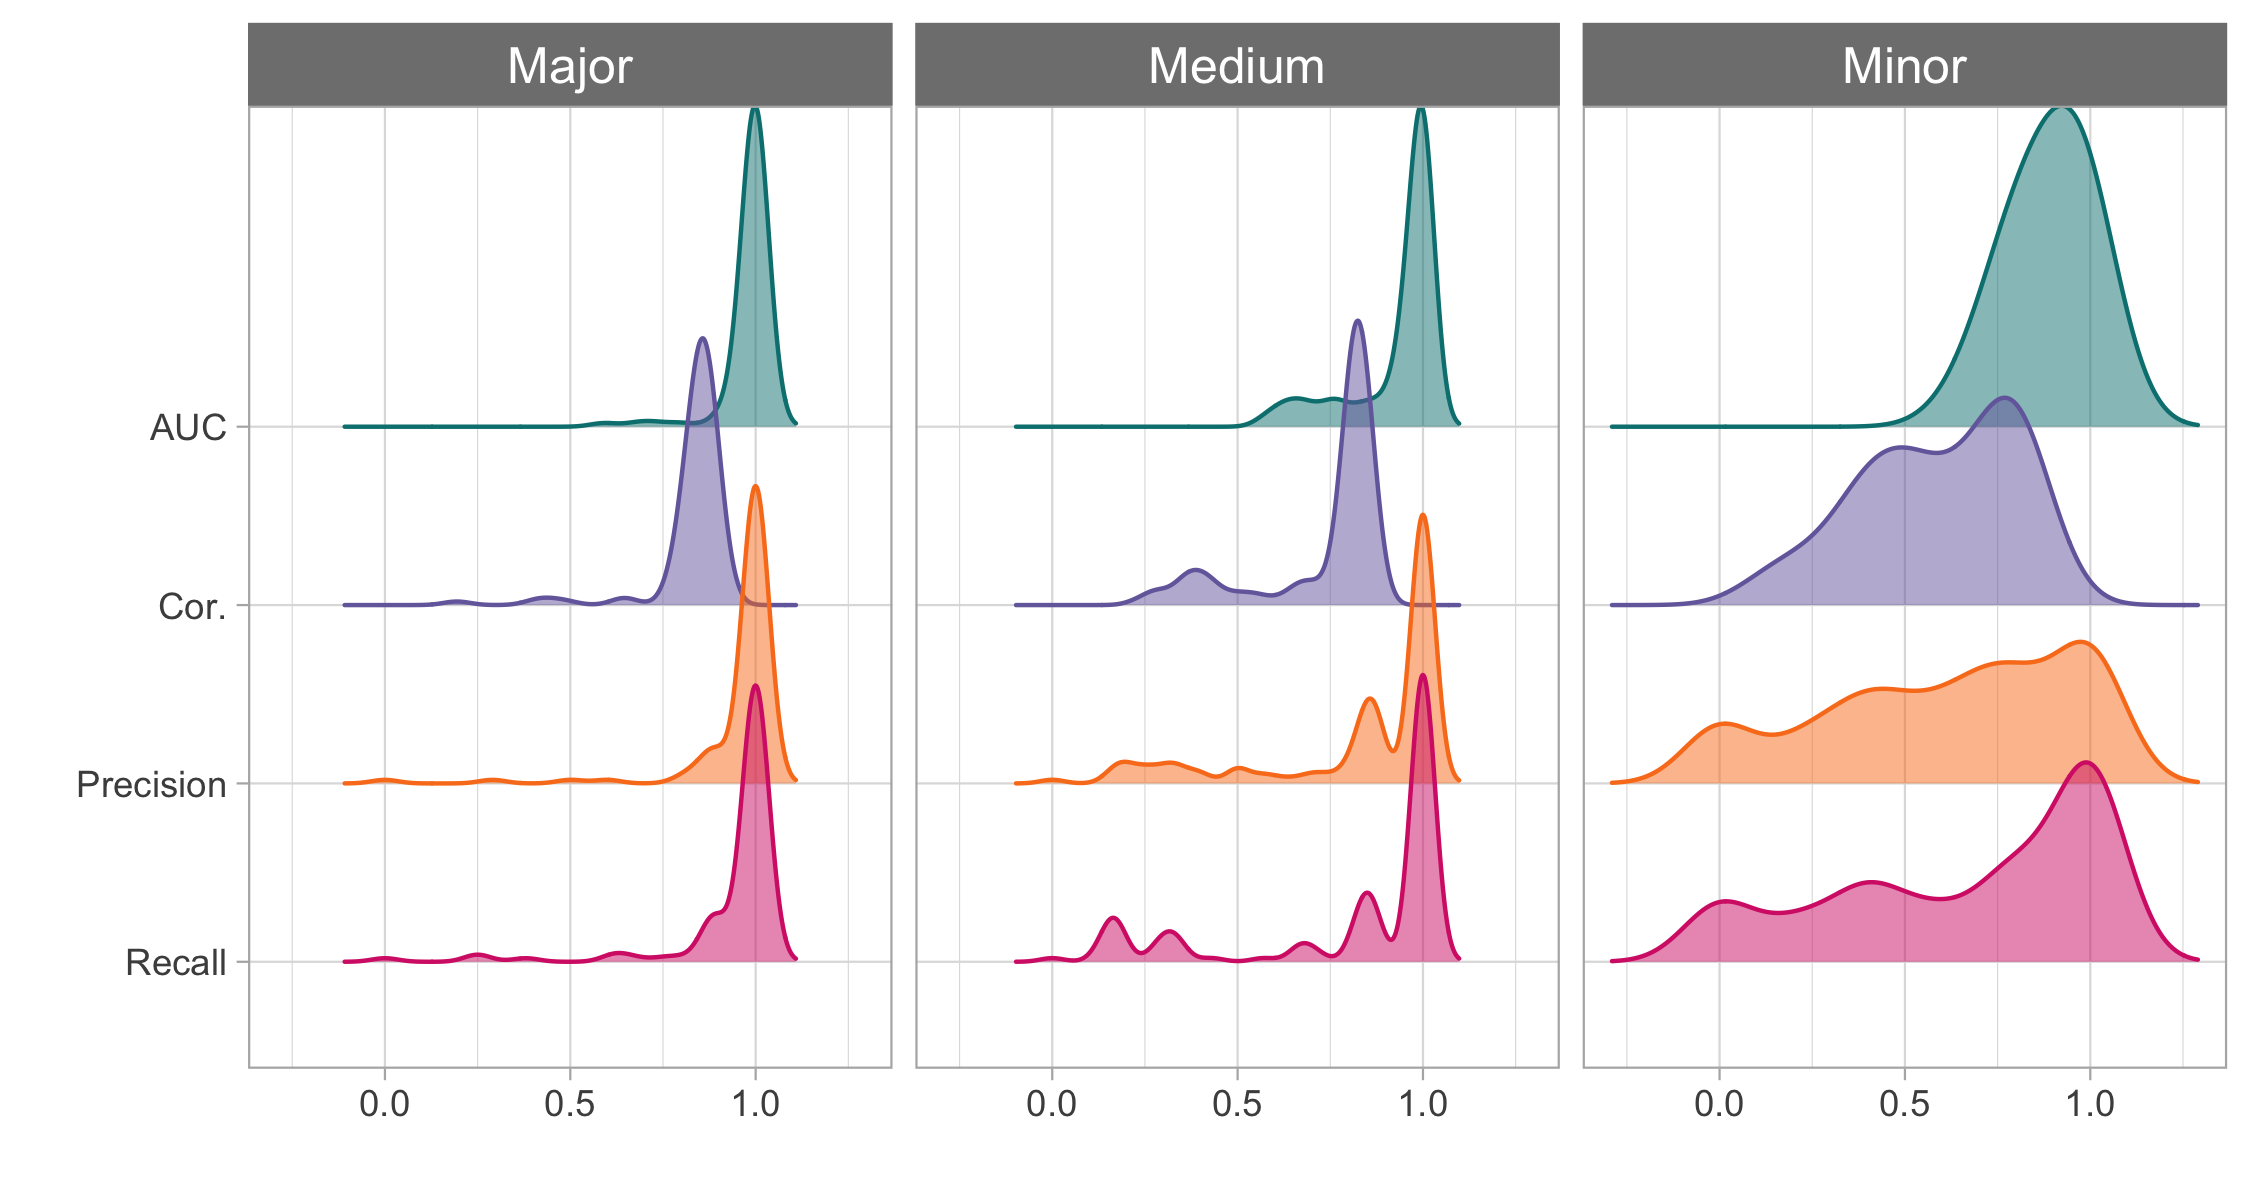
\includegraphics[width=11cm]{figs/simu_densities.png}
    \caption{
    %\CA{}
    The influence of the missing actor is measured with its degree, distinguishing three influence classes: \textit{Minor} (degree $\leq 5$), \textit{Medium} ($5<$ degree $\leq 7$) and \textit{Major} (degree $\geq 8$). 
    %\CA{Distributions of performance measures}
    The distributions of performance measures are displayed for each class of influence: AUC measures the retrieval of the dependence structure between all variables, observed and missing.  Precision and recall are specific to the missing actor links. 
    }
    \label{fig:densities}
\end{figure}
 

\begin{figure}[H]
    \centering    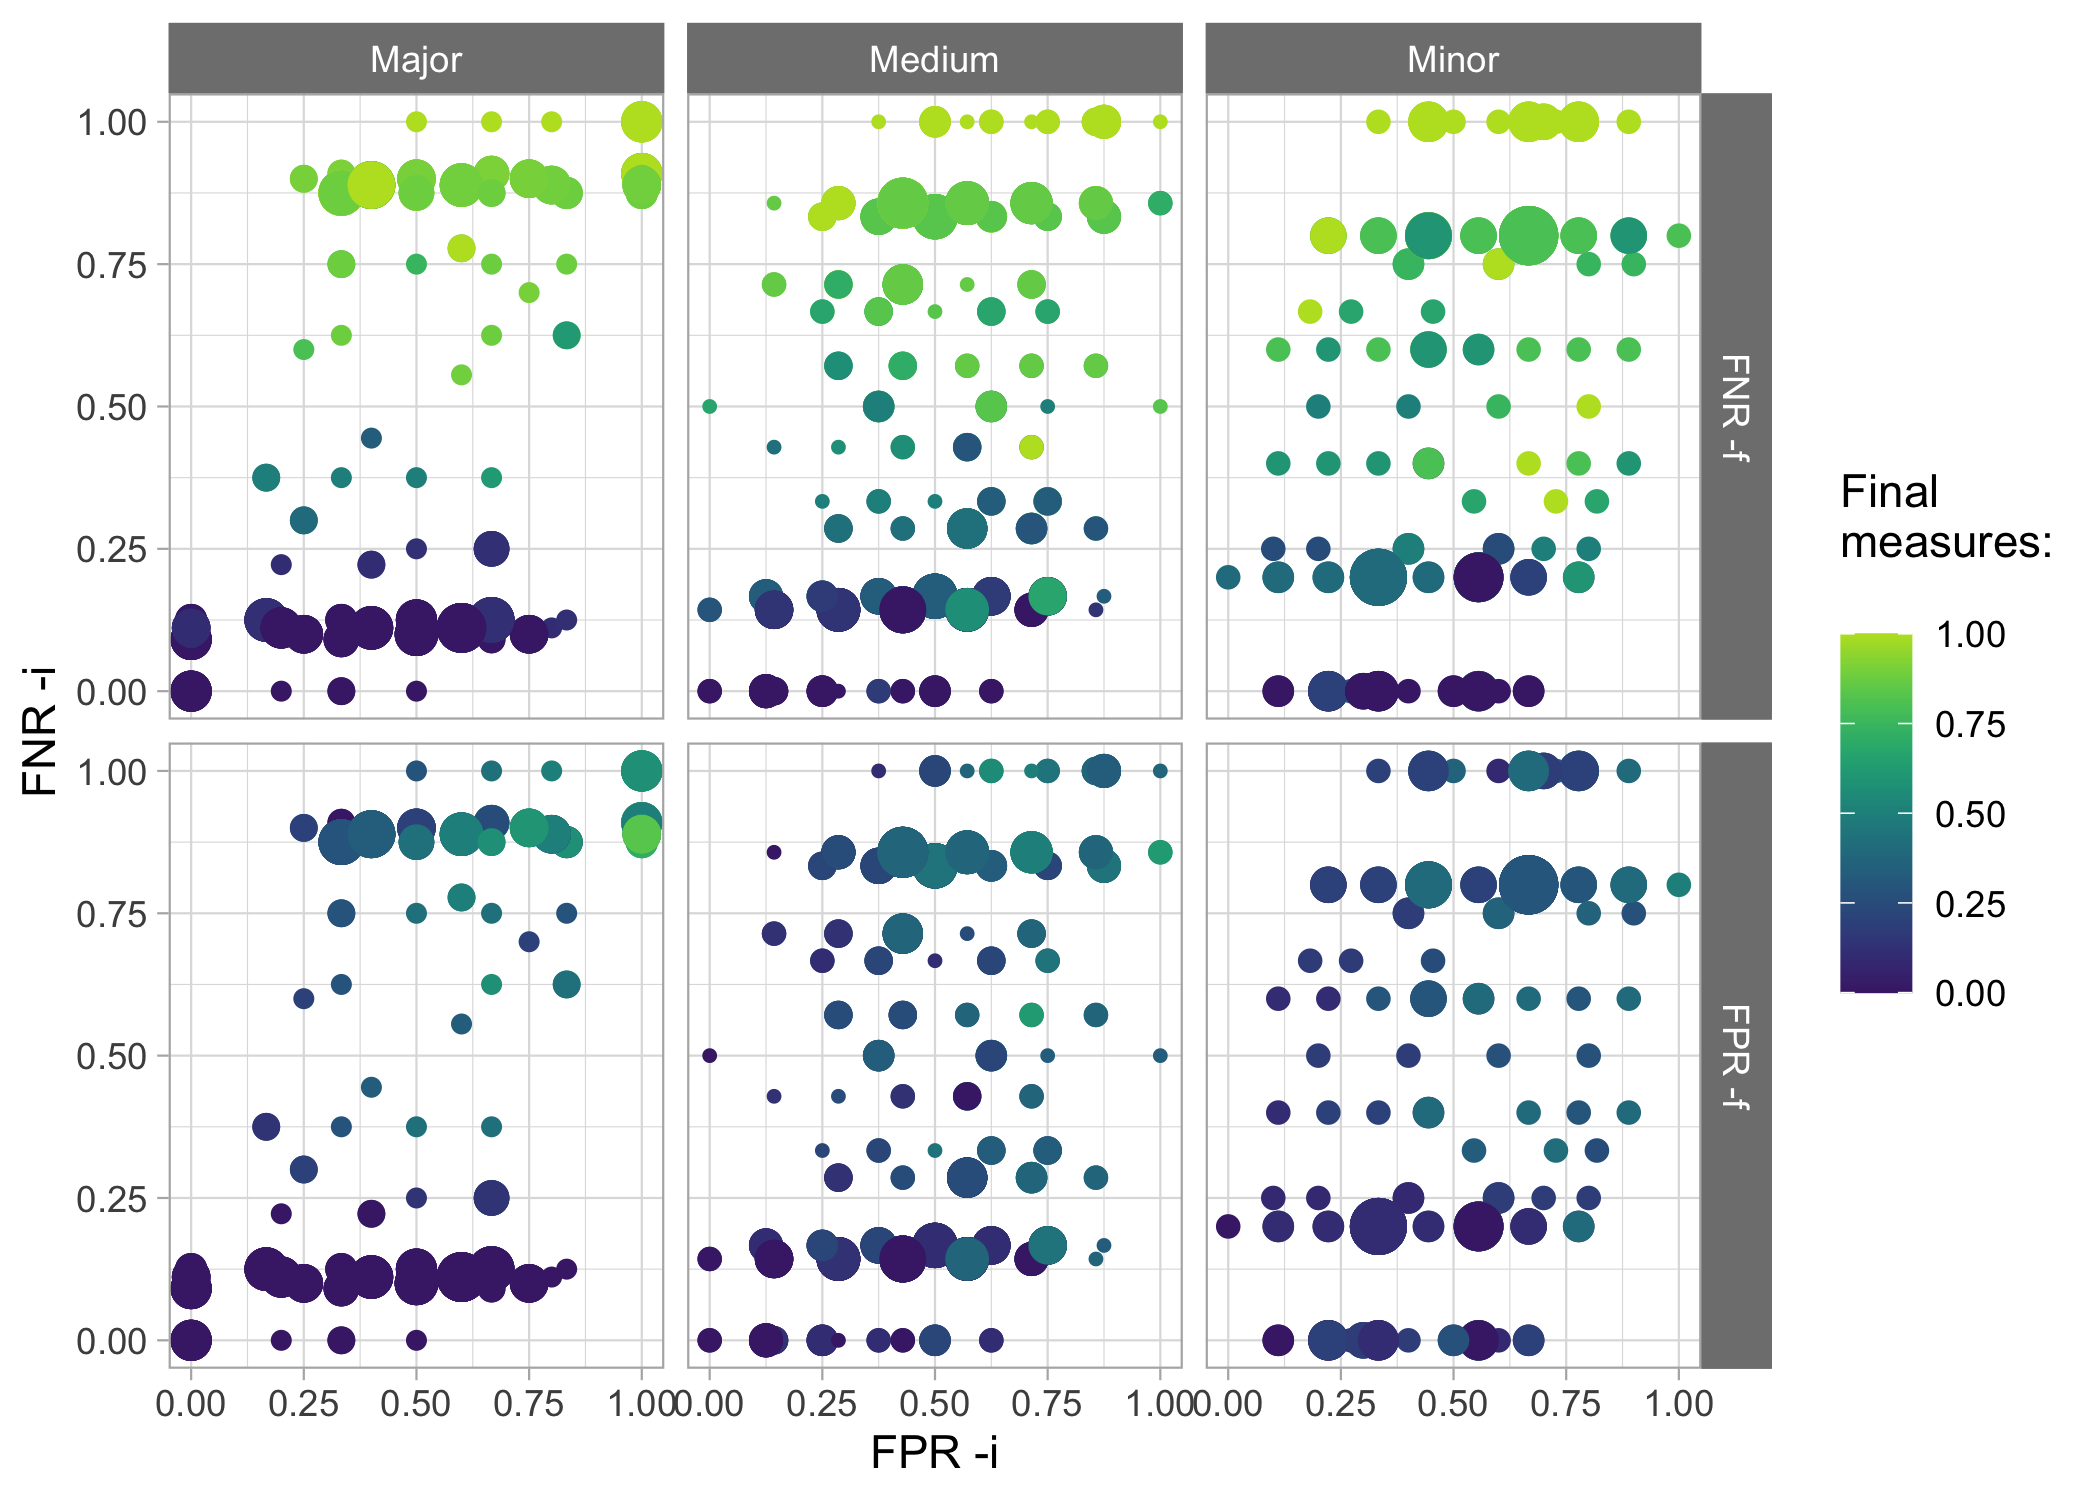
\includegraphics[width=11cm]{figs/quali_init_spca.png}
    \caption{Comparison of initial and final FPR and FNR, for cliques of neighbors of one missing actor obtained with the sparse PCA method. Position of dots are defined according to initial values, their color according to the final FPR and FNR. Sizes are proportional to the density of dots on a given position.}
    \label{fig:perfinit}
\end{figure}


 \begin{table}
\centering
\begin{tabular}{lrrrrrr}
  \hline
  & N & AUC & Precision & Recall & Cor. &t(s) \\ 
  \hline
  Major & 100 & 1 (0.00) & 1 (0.00) & 1 (0.01) & 0.86 (0.02)  & 1.28 (0.21) \\ 
  Medium & 132 & 1 (0.02) & 1 (0.00) & 0.99 (0.04) & 0.83 (0.02)  & 1.38 (0.46)  \\ 
  Minor &  68 & 0.98 (0.04) & 0.99 (0.03) & 0.96 (0.12) & 0.8 (0.04)& 1.56 (0.69) \\ 
   \hline
\end{tabular}
 \caption{\label{tab:oracle} Oracle procedure using true clique as starting point. The influence of the missing actor is measured with its degree, distinguishing three influence classes: \textit{Minor} (degree $\leq 5$), \textit{Medium} ($5<$ degree $\leq 7$) and \textit{Major} (degree $\geq 8$).  For each class of influence, the following quantities are reported:  number of simulated graphs (N), means and standard deviations of AUC, Precision, Recall, Correlation between missing actor inferred vector of means and original latent vector, and running times in seconds. AUC measures the retrieval of the dependence structure between all variables (observed and missing), whereas precision and recall are specific to the missing actor links.}
\end{table}


\section{Applications}  \label{sec:Appli}


%%%%%%%%%%%%%%%%%%%%%%%%%%%%%%%%%%%%%%%%%%%%%%%%%%%%%%%%%%%%%%
\subsection{Cross validation criterion for  model selection}
%\SR{
%As no model selection criteria has been designed for this problem yet, we  run a 10-fold cross-validation procedure, with pairwise composite likelihood (PCL) as adjustment criteria (see \citet{lindsay}). This choice of pairwise components is motivated from the fact that they keep track of the covariance structure, and the estimation of bivariate Poisson log-normal densities is made possible thanks to the \texttt{bipoilog} function of the \texttt{poilog} R package. \\
%
%The cross-validation procedure to estimate the pairwise composite likelihood is available in appendix \ref{CV}. The general idea is to compute the bivariate Poisson log-normal densities between all pair of species, conditional on a tree sampled as explained in appendix \ref{sampTrees} which defines the distribution parameters. Finally the procedure computes the average criteria  $$\displaystyle PCL(\Ybf)=\frac1V\sum_{v=1}^{V}\frac1B \sum_{b=1}^Bf_{PLN}(\Ybf; b,v),$$ where $f_{PLN}(\Ybf; b,v)=\sum_{\substack{i \in v\\ j < k}} \log p_{PLN}[(Y_{ij}^v, Y_{ik}^v) | T^b; \widehat{\theta},\widehat{\Sigma}_{T^b jk}]$, with $V=10$ and $B=10^2$. \\
%This is a computational greedy procedure that is not suited for a simulation study. It was applied to two empirical datasets in order to decide the number of missing actors in the model. The results, gathered in Figure \ref{fig:selec}, yield $r=1$ for the Barents Sea data set, and $r=2$ for the Fatala River one.}{}

The proposed model obviously raises the problem of choosing the number of missing actors $r$ (which may be zero). Variational-based inference often relies on approximate versions of the BIC or ICL criteria for model selection. Few theoretical guaranties exist about these approximate criteria and, in the present case, we observed that BIC and ICL penalizations did not yield consistent results. Therefore, we resort to $V$-fold cross validation to determine the number of missing actors. 

More specifically, we split the original dataset $\Ybf$ ($\Xbf$ is dropped here for the sake of clarity) into $V$ subsets with almost equal sizes $m_1, \dots m_V$ ($\sum_{v=1}^V m_v = n$), which we denote $\{\Ybf^v\}_{v = 1, \dots V}$. For each subset $v$, we define its complement $\Ybf^{-v}$ on which we fit a model with $r$ missing actors and get a parameter estimate $\Gammabf_r^{-v} = (\thetabf_r^{-v}, \sigmabf_r^{-v}, \betabf^{-v}_r, \Omegabf_r^{-v})$ and measure the fit of $\Gammabf_r^{-v}$ to the test dataset $\Ybf^v$. 

To avoid the integration over the $(p+r)$-dimensional Gaussian latent layer, we measure the fit with the pairwise composite likelihood \citep{lindsay}.
For any given tree $T$ and parameter $\Gammabf$, the bivariate Poisson log-normal pdf $p_{PLN}\left((Y_{ij}, Y_{ik}); \Gammabf, T \right)$ can be easily computed for any sample $i$ and pair of species $(j, k)$ with available tools such as the \texttt{poilog} R package \citep{ViS08} available on CRAN. The cross-validation criterion is defined as
$$
PCL_r(\Ybf) = \frac1V \sum_v \frac1B \sum_{b=1}^B \frac1{m_v} \sum_{i = 1}^{m_v} \sum_{j < k} \log p_{PLN}\left((Y^v_{ij}, Y^v_{ik}); \Gammabf_r^{-v}, T_{r, b}^{-v} \right)
$$
where the tree samples $\{T_{r, b}^{-v}\}_{b=1 \dots B}$ are iid according to $p_{\betabf_r^{-v}}(T)$. 

The sampling procedure for spanning trees is given in Appendix \ref{eq:sampTree}; the complete procedure for the calculation of $PCL_r(\Ybf)$ is described by Algorithm \ref{algo:model-selection}, given in Appendix \ref{sec:modSel}. Note that this criterion measures the fit of the model in terms of abundance prediction, whereas our interest is mostly focused on the inference of the dependency structure. In other words, our goal is identification, that is selecting the smallest model  and not the best model in terms of prediction \citep{arlot2010survey}.


We did not include this computationally greedy procedure in the simulation study but applied it to the two ecological datasets that will be described in the next two sections. The results, gathered in Figure \ref{fig:selec}, yield $r=1$ missing actor for the Barents Sea data set, and $r=2$ missing actors for the Fatala River one.

\begin{figure}[H]
    \centering
    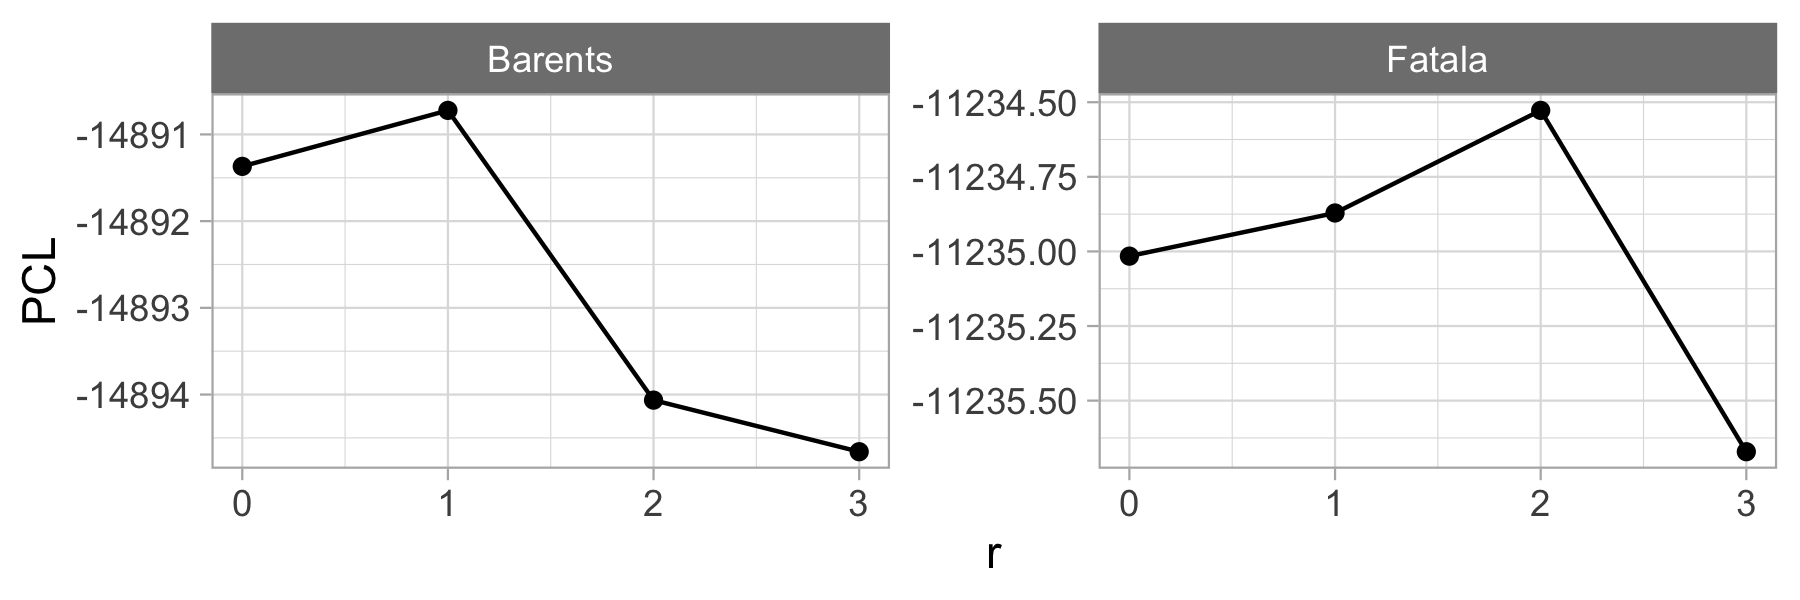
\includegraphics[width=10cm]{figs/selec_model_applis.png}
    \caption{Pairwise composite likelihoods estimates of Barents and Fatala datasets for models including 0 to 3 missing actors.}
    \label{fig:selec}
\end{figure}

% \SR{
% A wider exploration of likely cliques is conducted thanks to a bootstrap approach with $200$ sub-samples. Each of the latter consists of 80\% of the data; sPCA is run on each of them and only the identified clique of the $r$ first principal components are stored, when the studied model involves $r$ missing actors. When $r>1$, the restriction on the clique sizes is lifted. The bootstrap thus yield 200 lists of $r$ initial cliques, from which only unique ones are kept. This approach is more time-consuming, and therefore only used on empirical datasets.
% }{
Regarding the initialization, we performed a wider exploration as compared to the simulation study. To enlarge the list of possible cliques, we applied a resampling version of the procedure described in Section \ref{sec:algoSpec}, and applied it to 200 sub-samples, each consisting in 80\% of the whole data set. This yielded 200 lists of $r$ initial cliques, from which duplicates were removed.
%}

%%%%%%%%%%%%%%%%%%%%%%%%%%%%%%%%%%%%%%%%%%%%%%%%%%%%%%%%%%%%%%%%%%%%%%%%%%%%%%%%
\subsection{Barents Sea}
%data availability ? précisions sur les données, elles viennent d'où

% \SR{30 species of fish were counted in 89 sites of the Barents Sea (shrimp survey in the period April-May 1997, available at  \url{https://www.fbbva.es/microsite/multivariate-statistics/data.html})}{
The dataset was first published by \cite{FNA06} and consists of the abundance of 30 fish species measured in 89 sites in the Barents See in April-May 1997. In addition to abundances, the water temperature was measured in each site. The complete dataset is available at \url{www.fbbva.es/microsite/multivariate-statistics/data.html}. 
Fishes distributions are known to be greatly linked with the temperature. 
Hence to illustrate our methodology, 
% \SR{models were fit\CA{}{ted} without any covariates and with one missing actor, which we denote $h$. $\rm{Cor}(k,temp)$ denotes the absolute Pearson's correlation between $M_k$ (estimated vector of means of node $k$ along all 89 sites) and the temperature.}{
we present the results of the model fitted without any covariate (that is not accounting for the temperature), but including one missing actor (as suggested by Figure \ref{fig:selec}). To assess the ability of the proposed methodology to retrieve the influence of temperature as a missing actor, we report the empirical correlation between the temperature and the conditional expectation of the missing actor $M_h$, which we denote $\corHTemp$.
 
% Runing time
The resampling initialization procedure yielded in 14 different cliques, for each of which a VEM algorithm was run: the mean running time was $6.63$mins with deviation $0.70$ mins. 

% Dependency structure
The edge probabilities involving node $h$ as an endpoint were either very close to 0 or very close to 1, yielding a total of 6 highly probable neighbors of $h$. Figure \ref{fig:barents_adj} shows that many direct interactions are inferred between the corresponding 6 species in absence of a missing actor, which vanish when it is introduced. It also shows that accounting for this actor has only a local effect and that the direct interactions among the other species are preserved, which is consistent with our notion of a missing actor.

\begin{figure}[H]
    \centering
    \includegraphics[width=10cm]{figs/Barents_mat_comp.png} \\\vspace{-2cm}
    \includegraphics[width=10cm]{figs/Barents_net_comp3.png}
    \caption{\textit{Top left:} adjacency matrix of the Barents Sea fishes interaction network for $r=0$  missing actor. The inferred neighbors are gathered in the last 6 columns, so that their interactions are observable in the upper-right corner. \textit{Top right:} adjacency matrix for $r=1$  missing actor. The last column gathers the interactions of the inferred missing actor. \textit{Bottom}: Inferred interaction network with $r=0$ (left) and $r=1$ (right). Colored nodes refer to the inferred neighbors (blue) of the missing actor (yellow). The edges width are proportional to their probability.}
    \label{fig:barents_adj}
\end{figure}

%\begin{figure}[H]
%    \centering
%    \includegraphics[width=10cm]{missing_article/Fig/Barents_net_comp3.png}
%    \caption{Barents Sea fishes interaction network with $r=0$ (left) and $r=1$ (right). Colored nodes refer to the inferred neighbors (blue) of the missing actor (yellow).}
%    \label{fig:barents_net}
%\end{figure}

% Interpretation
In terms of interpretation, Figure \ref{fig:barents_temp} shows that the missing actor is highly correlated with the temperature. It also appears that the abundances of the species neighbor to the missing actor are much more correlated with the temperature (mean correlation = 0.78, sd = .06) than the abundances of the non-neighbor species (mean correlation = 0.46, sd = .27). This example shows the ability of the method to recover an underlying effect that would not be recorded in the data.

\begin{figure}
    \centering
    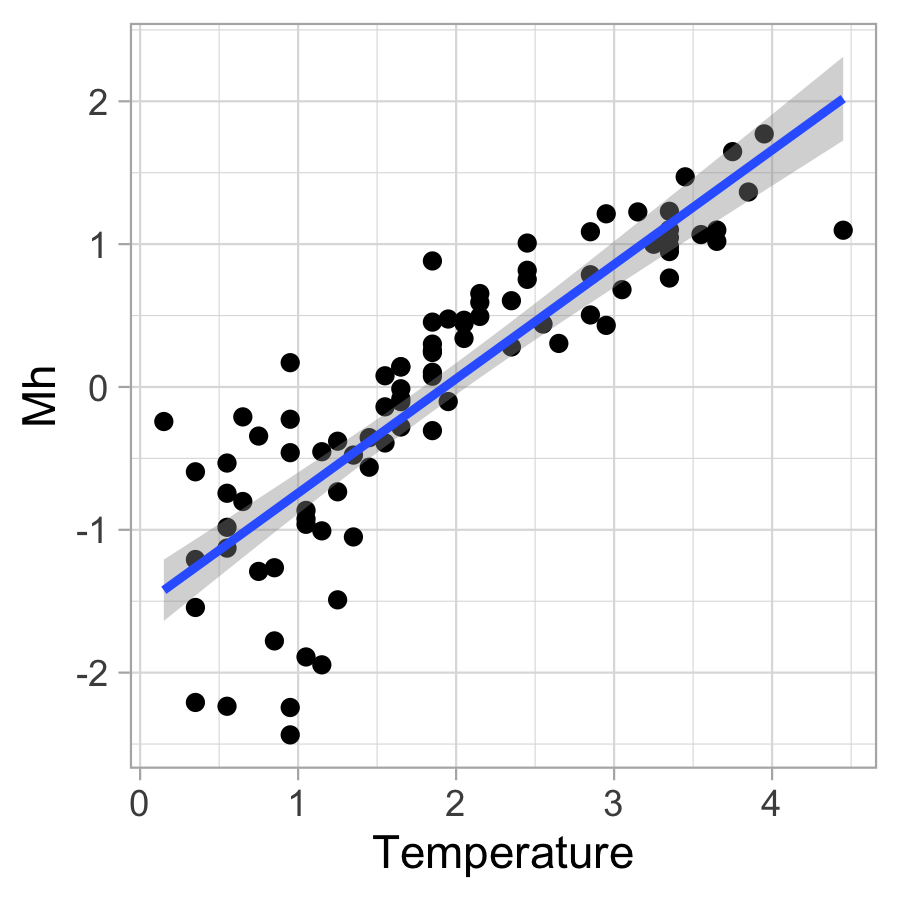
\includegraphics[width=5cm]{figs/Barents_MH_temp_white.png}
    \caption{Missing actor estimated vector of means $M_h$ as a function of the temperature. $\corHTemp=0.85$.}
    \label{fig:barents_temp}
\end{figure}

% \SR{
% Table \ref{tab:barents} then gathers the mean of correlations to the temperature of neighbors and non-neighbors. It appears that neighbors to the missing actor are significantly more correlated to the temperature than other nodes are.
% \begin{table}[ht]
% \centering
% \begin{tabular}{rlrr}
%   \hline
%   $P_{hk}$ & $\corKTemp$  \\ 
%   \hline
%  $<0.5$  & 0.44 (0.25)\\ 
%   $\geq 0.5$ & 0.80 (0.06) \\ 
%   \hline
% \end{tabular}
% \caption{Mean and standard deviation of $\corKTemp$ in relation with node $k$ being inferred as a neighbor ($P_{hk}\geq 0.5$) of missing actor $h$ or not ($P_{hk}< 0.5$).}
% \label{tab:barents}
% \end{table}
% }{
%} 

%\begin{figure}
%    \centering
%    \includegraphics[width=9cm]{missing_article/Fig/Barents_mat_comp.png}
%    \caption{\textit{Left:} adjacency matrix of Barents Sea fishes interaction network for $r=0$. The inferred neighbors are gathered in the last 6 columns, so that their interactions are observable in the upper-right corner. \textit{Right:} adjacency matrix of Barents Sea fishes interaction network for $r=1$. The last column gathers the interactions of the inferred missing actor.}
%    \label{fig:my_label}
%\end{figure}

%\begin{figure}[H]
%    \centering
%    \includegraphics[width=10cm]{missing_article/Fig/Barents_net_comp3.png}
%    \caption{Barents Sea fishes interaction network with $r=0$ (left) and $r=1$ (right). Colored nodes refer to the inferred neighbors (blue) of the missing actor (yellow).}
%    \label{fig:my_label}
%\end{figure}

%%%%%%%%%%%%%%%%%%%%%%%%%%%%%%%%%%%%%%%%%%%%%%%%%%%%%%%%%%%%%%%%%%%%%%%%%%%%%%%%
\subsection{Fatala River}
% \SR{
% The R package \texttt{ade4}  provides with the baran95 dataset which gathers the abundances of 33 species of fish on 90 locations of the Fatala River in Guinea. Data sampled between June 1993 and February 1994, which we organize in dry and rainy seasons; dates and sites are available as dataset categorical covariates.
% %
% Again models are fit with no covariates, and here two missing actors are inferred, which we denote $h1$ and $h2$. As models include more than one missing actor, the best VEM is selected under the constraint $\log sd(M_h)\geq -20$ for $h\in \{h1, h2\}$. This constraint ensures that the corresponding marginal variance of each missing actor is not too high, which would mean that the algorithm did not learn a lot about them. In other words, this ensures the algorithm succeeds in finding the desired number of missing actors. \\
% %
% The bootstrap method gives 60 unique  lists of two possible initial cliques and the mean running time for a convergence with precision $1e-3$ is $11.33$ min with deviation $1.47$; 14 did not reach convergence and the algorithm stopped after 100 iterations. \\
% %
% The best fit gives vectors of means $Mh1$ and $Mh2$ corresponding two each missing actor. Figure \ref{fig:Fatala} shows the plot of $Mh1$ against $Mh2$ colored with either one of the available covariates. It is very interesting to see that $Mh1$ is linked to the Site covariate, as it clearly separates kilometer 3 from kilometer 46 which are the first and last locations. On the other hand $Mh2$ seems linked with the Season covariate, even if the separation is less obvious.
% }{
\cite{baran1995dynamique} collected the abundances of 33 fish species in 90 sites along the Fatala River in Guinea between June 1993 and February 1994. The data are available from the R package \texttt{ade4} on CRAN \citep{dray2007ade4}, along with the date and site of collection, from which we deduce the season (dry or rainy). Again the model was fitted without any covariates, but with two missing actors, as suggested by Figure \ref{fig:selec}. \\
%
The resampling initialization procedure yielded in 60 different cliques, for each of which a VEM algorithm was run: the mean running time was $11.33$ min (sd = $1.47$ mn). 14 VEM did not reach convergence (with tolerance $\varepsilon = 1e-3$) after 100 iterations. We filtered out the results obtained from the different initializations, when the algorithm obviously ended in a degenerate solution ($\Var(M_h) < \exp(-20)$). \\ 
%
% %\SR{
% Figure \ref{fig:Fatala} shows the scatterplot of estimated conditional mean of the two missing actors $(M_{h_1}, M_{h_2})$ in each site, colored with either one of the available covariates (site and season). $M_{h_1}$ is obviously linked to the site and separates most upstream locations (kilometer 3) from most downstream locations (kilometer 46). On the other hand $M_{h_2}$ seems linked with the Season covariate, even if the separation is less obvious. Similarly, the second missing actor shows a clear relation with the season. \\
% % 
% Again, the retrieved missing actor each correspond to an underlying effect that rules fish species abundances. The clear separation between the two effects is reinforced by the assumption the missing actors are independent from each other, which obviously holds for locations ans seasons. \\
% }{
Figure \ref{fig:Fatala} shows the scatterplot of the estimated conditional mean of the two missing actors $(M_{h_1}, M_{h_2})$ in each site, colored with either one of the available covariates (site and season). The missing actor $h_1$ is obviously linked to the site and separates most upstream locations (kilometer 3) from most downstream locations (kilometer 46). This actor has 11 highly probable neighbor species.
% \textcolor{red}{comparer les anova Poisson pour les voisins / pas voisins}
Again, this retrieved missing actor corresponds to an underlying effect (in this case: geography) that rules fish species abundances. \\
% 
The second missing actor seems to be linked with the season but with a less clear separation. Also the variability of $M_{h_2}$ is much smaller than this of $M_{h_1}$. This effect is therefore questionable, which brings us back to model selection. As mentioned above, we used a procedure based on cross-validation, which may  be prone to select too complex model \citep{shao1993linear,friedman2001elements,arlot2010survey}. The definition of a grounded model selection criterion for structure inference in presence of missing actors remains open.
%}

%\textcolor{red}{[C'est un peu dommage de finir comme ça mais bon...]}
 
\begin{figure}[h]
    \centering
    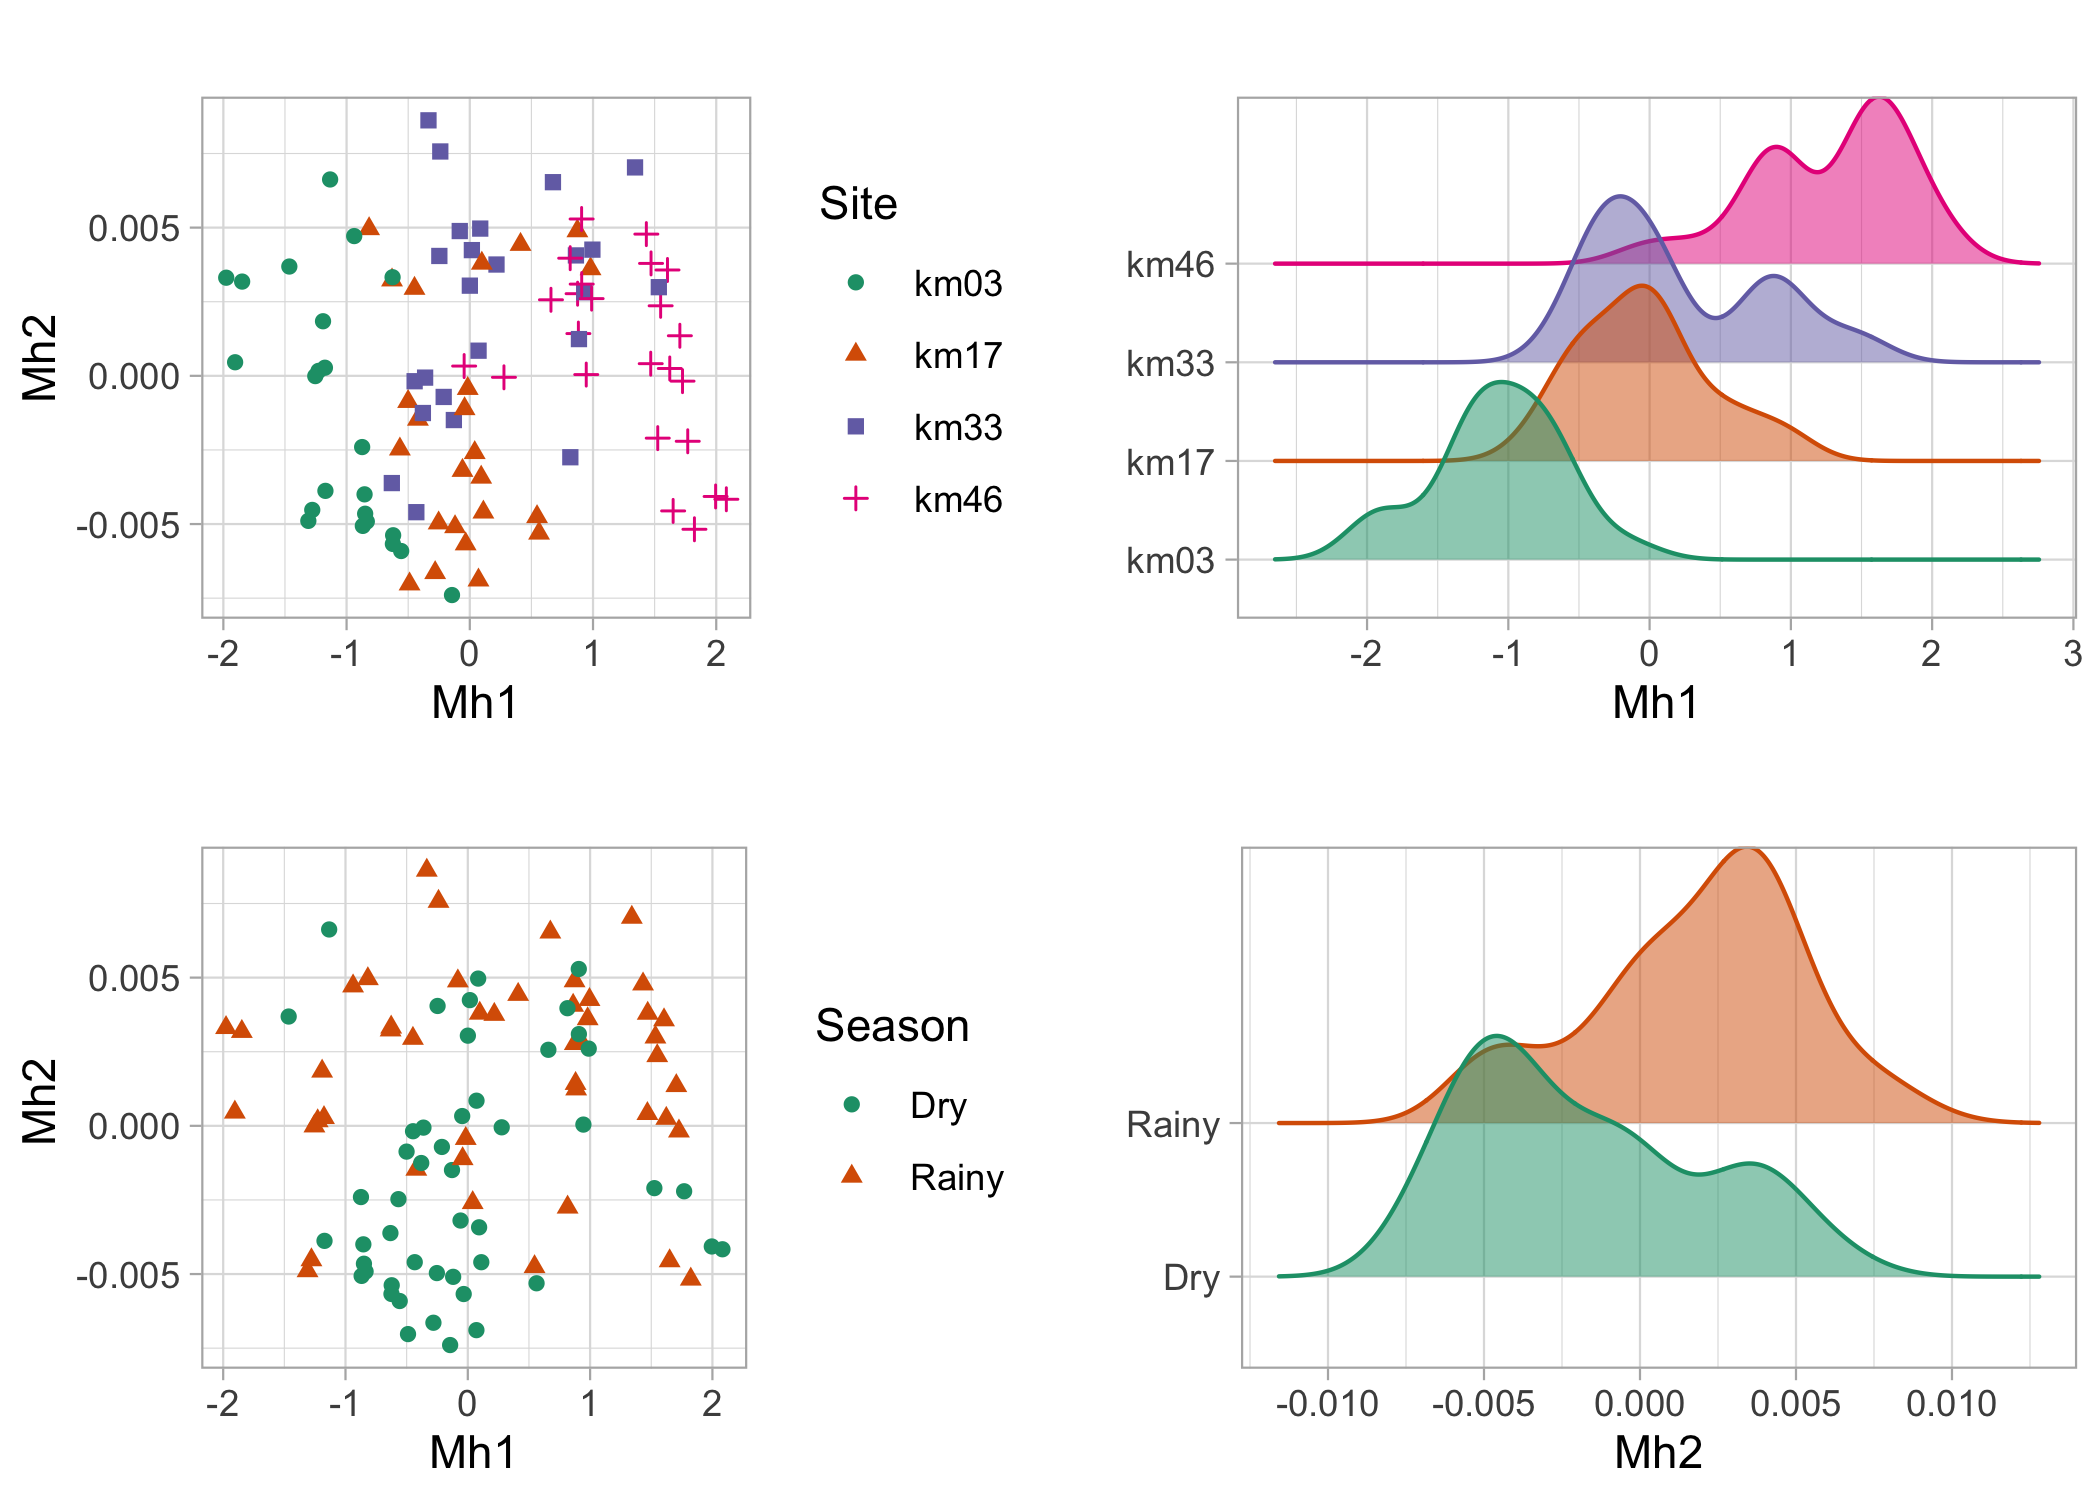
\includegraphics[width=12cm]{figs/Fatala_MH2.png}
    \caption{Estimated means $M_{h_1}$ and $M_{h_2}$ of the two inferred missing actors. Left column: scatterplots $M_{h_1}$ vs $M_{h_2}$ with site (top) and season (bottom) color code. Right: distribution of the estimated means across sites. Top right: distribution of $M_{h_1}$ in each location, bottom right: distribution of $M_{h_2}$ in each season.}
    \label{fig:Fatala}
\end{figure}



\begin{subappendices}
%\addtocontents{toc}{\setcounter{tocdepth{-1}}
\section{Published supplements}
 \tocless \subsection{Algebraic Tools} \label{app:tools}
 We here present some algebraic results about spanning tree structures which are used during the computations. Theorem \ref{thm:MTT}, Lemma \ref{lem:Meila} as well as Lemma \ref{lem:Kirshner} use the notion of Laplacian matrix  $\Qbf$ of a symmetric matrix $\Wbf=[w_{jk} ]_{1\leq j,k\leq p}$, which is defined as follows :
 
\[
 [\Qbf]_{jk}  =\begin{cases}
    -w_{jk}  & 1\leq j<k \leq p\\
    \sum_{u=1}^p w_{ju} & 1\leq j=k \leq p.
    \end{cases}
\]
 
We further denote $\Wbf^{uv}$ the matrix $\Wbf$ deprived from its $u$th row and $v$th column and we remind that the $(u, v)$-minor of $\Wbf$ is the determinant of this deprived matrix, that is $|\Wbf^{uv}|$.
The following Theorem \ref{thm:MTT} is the extension of Kirchhoff's Theorem to the case of weighted graphs \citep{matrixtree,MeilaJaak}.\\
\begin{theorem}[Matrix Tree Theorem] \label{thm:MTT}
    For any symmetric weight matrix W with all positive entries, the sum over all spanning trees of the product of the weights of their edges is equal to any minor of its Laplacian. That is, for any $1 \leq u, v \leq p$,
   \[
    W := \sum_{T\in\mathcal{T}} \prod_{(j, k)\in T} w_{jk} = |\Qbf^{uv}|.
    \]\\
\end{theorem}    

In the following, without loss of generality, we will choose $\Qbf^{11}$. As an extension of this result, \cite{MeilaJaak} provide a close form expression for the derivative of $W$ with respect to each entry of $\Wbf$. 

\begin{lemma} [\cite{MeilaJaak}] \label{lem:Meila}
    Define the entries of the symmetric matrix $\Mbf$ as
 \[    
 [\Mbf]_{jk} =\begin{cases}
    \left[(\Qbf^{11})^{-1}\right]_{jj} + \left[(\Qbf^{11})^{-1}\right]_{kk} -2\left[(\Qbf^{11})^{-1}\right]_{jk} & 1< j<k \leq p\\
    \left[(\Qbf^{11})^{-1}\right]_{jj} & k=1, 1< j \leq p  \\
    0 &  j=k .
    \end{cases}
\]
it then holds that $$\partial_{w_{jk}} W = [\Mbf]_{jk}  \times W.$$\\
\end{lemma}

\cite{kirshner} build on Lemma \ref{lem:Meila} to provide an efficient computation of all edges probabilities.
\begin{lemma} [\cite{kirshner}] \label{lem:Kirshner}
    Let $p_W$ be a distribution on the space of spanning trees, such that $p_W(T)=\prod_{kl\in T} w_{kl} / W$, where $W$ is defined as in Theorem \ref{thm:MTT}. Taking the symmetric matrix $\Mbf$ as defined in Lemma  \ref{lem:Meila}, the probability for an edge $kl$ to be in the tree $T^*$ writes:
 
$$\mathds{P}\{kl\in T^*\} = \sum_{T\in \mathcal{T}} p_W(T)= w_{kl}\: \Mbf_{kl}$$
\end{lemma}



\tocless\subsection{Computations} \label{app:comput}
\subsubsection[Update of tree parameter vector]{Update of $\betabf$.} \label{up:beta}
As in \citet{MRA20}, the update of $\betabf$ is such that:
$$\betabf^{t+1}  = \arg\max_\betabf \; \Esp_{g^t} \left[ \log p_\betabf(T) \right].
$$
By definition of $p_\betabf(T)$:
$$\Esp_{g^t} \left[ \log p_\betabf(T) \right] = \sum_{kl} P^t_{kl} \log \beta_{kl} - \log B\;,
\qquad
B=\sum_{T\in \mathcal{T}}\prod_{kl\in T} \beta_{kl}.$$
Computing the derivative with respect to the edge weight $\beta_{kl}$ gives:
\begin{align*}
\partial_{\beta_{kl}}\Esp_{g^t} \left[ \log p_\betabf(T) \right] &=\frac{P_{kl}^t}{\beta_{kl}} - \frac{\partial_{\beta_{kl}} B^t }{B^t}.
\end{align*}
According to Lemma \ref{lem:Meila}: $\partial_{\beta_{kl}} B^t  = [\boldsymbol{M}]_{kl} \times B$. Finally setting the derivative to 0 yields the update formula $
\beta^{t+1}_{kl} 
= \frac{P^t_{kl}}{ M(\betabf^t)_{kl}}$.

\subsubsection[Update of Gaussian tree precision matrix]{Update of $\Omega_T$} \label{up:omega}
The update of $\Omegabf_T$ respects
$$\Omegabf^{t+1}  = \arg\max_\Omegabf \; \Esp_{q^t} \left[ \log p_{\Omegabf}(\Ubf \mid T) \right].$$
This is a problem of parameter optimisation in the context of Gaussian Graphical Models (GGM).
In what follows, for any $q\times q$  matrix $A$, $A_{[kl]}$ will refer to the block $kl$ of $A$: $A_{[kl]}=(a_{ij})_{\{i,j\}\in\{k,l\}}$.   $[A_{[kl]}]^q$ will then denote the matrix obtained by filling up with zero entries to obtain full dimension $q\times q$, so that:
$$([A_{[kl]}]^q )_{ij}=\left\{ \begin{array}{rl}
a_{ij} & \text{if } \{i,j\}\in\{k,l\}\\
0 &  \text{if } \{i,j\}\in\{1,..., q\}_{\setminus kl}
\end{array}\right.$$
In its proposition 5.9, \citet{Lau96} states that in a  GGM with $p$ variables and associated with the decomposable graph $\mathcal{G}$, the maximum likelihood of the precision matrix exists if and only if $n > \max_{C\in \mathcal{C}} |C|$. It is then given as 
$$\widehat{\Omega}=n\left(\sum_{C\in \mathcal{C}} [SSD_{[C]}\,^{-1}]^p - \sum_{S\in \mathcal{S}} \nu(S)\,[SSD_{[S]}\,^{-1}]^p \right)$$
where $\mathcal{C}$ is the set of cliques and $\mathcal{S}$ the set of separators of $\mathcal{G}$, with associated multiplicities $\nu(S)$.\\


In our context, $\mathcal{G}$ is a spanning tree and so all cliques are edges and separators are nodes. The multiplicity of a given node $k$ as a separator in the graph is  $\nu(k) = d(k)-1$, where $d(k)$ is its degree. Therefore the estimator  $\widehat{\Omega}_T$  writes as the following 
\begin{align*}
\widehat{\Omega}_T &= n  \sum_{kl\in T}   [(SSD_{[kl]})^{-1}]^{p+r} - n\sum_k (d(k)-1)[(SSD_{kk})^{-1}]^{p+r}\\
&=n \sum_{kl\in T}  [(SSD_{[kl]})^{-1} - (SSD_{kk})^{-1} -  (SSD_{ll})^{-1} ]^{p+r} + n\sum_k[(SSD_{kk})^{-1}]^{p+r}
\end{align*}
As $SSD$ has diagonal $n$, the expression simplifies. Denoting $I_d$ the identity matrix of dimension $d$ we obtain:
$$\widehat{\Omega}_T =n\sum_{kl\in T} [(SSD_{[kl]})^{-1} -\frac{1}{n} I_2]^{p+r}+ I_{p+r}.$$

Detailing each bloc matrices as follows gives the update formulas in (\ref{omegaT}):
\[
n\times [(SSD_{[kl]})^{-1} - \frac{1}{n}I_2] = \frac{1}{1-(ssd_{kl}/n)^2}
\left(\begin{array}{cc}
		(ssd_{kl}/n)^2   & -ssd_{kl}/n\\
		-ssd_{kl}/n& (ssd_{kl}/n)^2 
		\end{array}\right)
\]


\subsubsection[for the toc]{Determinant of $\Omegabf_T$.}
The determinant of a precision matrix of a GGM with a decomposable graph is expressed as follows \citep{Lau96}:
$$ |\Omega| =\dfrac{\prod_{C\in \mathcal{C}} |\Sigma_C|^{-1}}{\prod_{S\in \mathcal{S}} |\Sigma_S|^{-\nu(S)}},$$
where $\Sigma = \Omega^{-1}$. As $\Omegabf_T$ is tree-structured, its determinant factorizes on the edges of $T$. It is expressed with the correlation matrix $\Rbf_T$ as follows, denoting $d(k)$ the degree of node $k$:
\begin{align*}
|{\Omegabf}_T| &=\frac{\prod_{kl \in T} |{\Rbf}_{Tkl}|^{-1}}{\prod_k |{\Rbf}_{Tkk}|^{1-d(k)}}.
 \end{align*}
Using that $\Rbf_T$ has diagonal 1, we obtain for step $t+1$ of the algorithm:
$$|\Omegabf^{t+1}_{T}| = \Big(\prod_{kl \in T} |\Rbf_{T[kl]}^{t+1}|\Big)^{-1}.$$


\subsubsection{Numerical issues.} \label{app:numIssues}

\paragraph{Exact computations} Our algorithm requires the computation of determinants (from the Matrix Tree Theorem) and inverses (in Kirshner's formula) of Laplacian of weight matrices. As we deal with highly variable weights, numerical issues arise: infinite determinants or matrix numerically non-invertible due to either the maximal machine precision (about $1.7\cdot 10^{308}$), or with machine zero (about $2.2 \cdot 10^{-16}$). To enhance the precision of such computations, we rely on multiple-precision arithmetic which allows the digit of precision of numbers to be  limited only by the available memory instead of 64 bits. We implemented matrix inversion and log-determinant computation using both, symbolic computation and multiple precision arithmetic, relying on the \texttt{gmp} R package available on CRAN, which uses \citep{lucas2020package}, the C library GMP (GNU Multiple Precision Arithmetic). 

\paragraph{Tempering parameter $\alpha$} \label{alpha}
\begin{description}
\item[\textit{Definition}: ]Weights $\widetilde{\beta}$ are mechanically linked to the quantity of data available $n$. To avoid reaching maximal precision when computing the determinant, a tempering parameter $\alpha$ is applied to every quantity proportional to $n$, so that the actual update performed is $$\log \widetilde{\beta}_{kl} = \log \beta_{kl} - \alpha(\frac{n}{2}\log|\widehat{\Rbf}_{Tkl}| + \widehat{\omega}_{Tkl} [M^\intercal M]_{kl}).$$
\item[\textit{Heuristic for an upper bound}: ] The proposed algorithm requires the computation of the normalizing constant $\widetilde{B}$, which is the determinant of any minor of the Laplacian  of the $q\times q$ variational weights matrix $\betabft$. As these weights  mechanically increase with the quantity of available data $n$, this step is numerically very sensitive.  Hereafter we denote $|\Qbf^{uv}|$ this determinant and $\Delta$ the maximal machine precision. In order to ease the computations, we define the tempering parameter $\alpha$ as $$\log \widetilde{\beta}_{kl} = \log \beta_{kl} - \alpha(\frac{n}{2}\log|\widehat{\Rbf}_{Tkl}| + \widehat{\omega}_{Tkl} [M^\intercal M]_{kl})\;,\qquad \text{under constraint}\;\;\; |\Qbf^{uv}| \leq \Delta.$$

Let's first detail the expression for $\widetilde{\beta}_{kl}$. Following the definition of the $SSD$ matrix, and update formulas \eqref{omegaT} and \eqref{RT}, we obtain:
\begin{align*}
    \log \widetilde{\beta}_{kl} &=\log \beta_{kl} +\alpha \,n\left\{\frac{(ssd_{kl}/n)^2}{1-(ssd_{kl}/n)^2} -\frac12\log\big[1-(ssd_{kl}/n)^2\big]\right\}.
\end{align*}
For large $n$, we thus have $$\widetilde{\beta}_{kl}\approx \exp \big[\alpha n \cdot C(ssd_{kl}/n)\big], \qquad \text{with }\; C(x)=x/(1-x) -\log(\sqrt{1-x}),\; x\in [0,1[.$$ 
We then define $C_{sup}$ such that $C_{sup} = C(ssd_{max})$, with $ ssd_{max}=\max\{ssd_{kl}, k\neq l\}$.
By definition, $\Qbf^{uv}$ is positive-definite, so its determinant is upper bounded by the product of its diagonal terms (Hadamard's inequality). Namely:
\begin{align*}
    |\Qbf^{uv}|&\leq \prod_{i=1}^{q-1} \Qbf^{uv}_{ii} \leq \prod_{i=1}^{q-1}\sum_{i=1}^{q-1} \exp (\alpha C_{sup} n)\\
    &\leq \left[(q-1)\exp(\alpha C_{sup} n)\right]^{q-1}.
\end{align*}
Then applying the constraint yields:
\begin{align*}
    |\Qbf^{uv}| \leq \Delta \iff  \alpha \leq \frac{1}{C_{sup} n} \left[ \frac{1}{q-1}\log \Delta - \log(q-1)\right].
\end{align*}

For $C_{sup}=0.8$, $n=200$ and $q=15$, we get $\alpha \leq 1.05\cdot 10^{-1}$.
\end{description}

%A heuristic for an upper bound of $\alpha$ is given in appendix \ref{alpha}.
%We provide a heuristic to set the parameter $\alpha$.


\tocless\subsection{Model selection and cross-validation} \label{sec:modSel}

%%%%%%%%%%%%%%%%%%%%%%%%%%%%%%%%%%%%%%%%%%%%%%%%%%%%%%%%%%%%%%%%%%%%%%%%%%%%%%%%%%%%%%%%
\subsubsection{Sampling spanning trees} \label{eq:sampTree}
%%%%%%%%%%%%%%%%%%%%%%%%%%%%%%%%%%%%%%%%%%%%%%%%%%%%%%%%%%%%%%%%%%%%%%%%%%%%%%%%%%%%%%%%%%%
Sampling non-uniform spanning trees (i.e. sampling $T$ from $p_\betabf$) is a research topic by itself, especially for large networks \citep[see][for a review]{DKP17}. For moderate size networks, a rejection algorithm \citep{Dev86} can be defined in the following way:
\begin{enumerate}
\item Sample $T$ from a distribution $q$, such that there exists a constant $M$, that ensures that, for all $T$, $M q(T) > p_\betabf(T)$;
\item Keep $T$ with probability $M^{-1} p_\betabf(T) / q(T)$ or try step 1 again.
\end{enumerate}
The efficiency of such an algorithm strongly relies on the choice of the proposal distribution. Here we adopt the following proposal:
\begin{enumerate}[label=\roman*]
\item Sample a connected graph $G$ with independent edges, each drawn with probability $Q_{jk} \propto P_{jk} = \mathds{P}_\betabf\{ jk \in T\}$; 
\item Sample $T$ uniformly among the spanning trees of $G$.
\end{enumerate}
%
\paragraph{Evaluation of the proposal.}
To evaluate the proposal distribution for each sampled tree, we may observe that, the probability for a graph drawn from the proposal to contain a given tree $T$ is approximately
$$
\mathds{P}_q\{G \ni T\} \approx \prod_{jk \in T} Q_{jk},
$$
the approximation being due to the connectivity constraint. This constraint can be almost surely satisfied by taking $Q_{jk}$'s large enough. So, denoting $|\Tcal(G)|$ the number of spanning trees in $G$, we have that
\begin{align*}
q(T) 
= \sum_{G \ni T} q(T \mid G) q(G)  = \sum_{G \ni T} \frac{q(G)}{|\Tcal(G)|} 
= \mathds{P}_q\{G \ni T\} \; \Esp\left(|\Tcal(G)|^{-1} \mid G \ni T \right).
\end{align*}
The last expectation can be evaluated via Monte Carlo, by sampling a series of graphs $G$ according to the proposal $q$ but forcing all edges from $T$ to be part of $G$. 
%
\paragraph{Upper bounding constant $M$.}
To evaluate the upper bounding constant $M$, we may observe that finding the tree $T^*$ such that
$$
m_\betabf 
:= \frac{\mathds{P}_q\{G \ni T^*\}}{p_\betabf(T^*)}
= \min_{T \in \Tcal} \frac{\mathds{P}_q\{G \ni T\}}{p_\betabf(T)} = \min_{T \in \Tcal} \prod_{jk \in T} \frac{Q_{jk}}{\beta_{jk}}.
$$
is a minimum spanning tree problem. Then, obviously, for any tree $T$: $\mathds{P}_q\{G \ni T\} \geq m_\betabf p_\betabf(T)$.
Now, because the maximum number of spanning trees within a graph is $p^{p-2}$, we have
$$
M q(T)
= M \sum_{G \ni T} \frac{q(G)}{|\Tcal(G)|} 
\geq \frac{M}{p^{p-2}} \sum_{G \ni T} q(G)
= \frac{M}{p^{p-2}} \mathds{P}_q\{G \ni T\}
\geq M \frac{m_\betabf}{p^{p-2}}  p_\betabf(T).
$$
So we may set $M = p^{p-2} / m_\betabf$. Still, in practice, this bound turns out to be far too large and needs to be tuned down to preserve computational efficiency.

%%%%%%%%%%%%%%%%%%%%%%%%%%%%%%%%%%%%%%%%%%%%%%%%%%%%%%%%%%%%%%%%%%%%%%%%%%%%%%%%%%%%%%%%%%%
 
\subsubsection{Cross-validation for model selection} \label{eq:cvAlgo}
\label{CV}

The cross-validation procedure to estimate the pairwise composite likelihood is given in Algorithm \ref{algo:model-selection}. In practice $V=10$ and $B = 100$.


\begin{algorithm}%[H]
\caption{Cross-validation for model selection with $r$ missing actors}
\label{algo:model-selection}
%  \dontprintsemicolon
  \CommentSty{// 0. INITIALIZATION}\; 
  Divide the dataset $\Ybf$ into $V$ subset $\Ybf^1, \dots \Ybf^V$;
  \BlankLine
  \For{$v \in \{1,\cdots, V\}$}{
    \BlankLine
    \CommentSty{// 1.   Apply the VEM algorithm to the train dataset $\Ybf^{-v}$}\; 
    $\Gammabf_r^{-v} \leftarrow (\thetabf_r^{-v}, \sigmabf_r^{-v}, \betabf^{-v}_r, \Omegabf_r^{-v})$
    \CommentSty{// 2. MONTE CARLO APPROXIMATION OF COMPLETE LOG-LIKELIHOOD EXPECTATION}\;
    \For{$b \in \{1,\cdots, B\}$}{
    \CommentSty{// 2.1 Draw tree (see Section \ref{eq:sampTree})}\; 
     $ T_{r, b}^{-v}  \sim p_{\betabf^{-v}_r}$ 
    \BlankLine
     \CommentSty{// 2.2. Build  the precision matrix having non-nul entries determined by $ T_{r, b}^{-v} $ and values stored in $\Omegabf_r^{-v}$, and its diagonal terms according to \eqref{omegaT}}\;
     $\Omegabf_{T^b}\leftarrow f( T_{r, b}^{-v} , \Omegabf_r^{-v} )$
     \BlankLine
      \CommentSty{// 2.3. Compute the marginal variance matrix }\;
      $\Sigmabf_{T^bO} \leftarrow  \Omegabf_{T^bOO} - \Omegabf_{T^bOH} \Omegabf_{T^bHH}^{-1} \Omegabf_{T^bHO}$;
          \BlankLine 
     \CommentSty{// 2.4. Compute the bivariate Poisson log-normal density in test sites}\;
     \For{site $i \in v$}{
        \For{pairs of species $(j,k)$}{
        $p_{PLN}\left((Y^v_{ij}, Y^v_{ik}); \Gammabf_r^{-v}, T_{r, b}^{-v} \right)$ with means $\xbf_i^\intercal \thetabf_{r, j}^{-v}$ and $\xbf_i^\intercal \thetabf_{r, k}^{-v}$ and variance matrix $[\Sigmabf_{T^bO}]_{[jk, jk]}$
%        $\log p_{PLN}[(Y_{ij}^v, Y_{ik}^v) | T^b; \widehat{\theta},\widehat{\Sigma}_{T^b jk}]$, 
         }}
       \CommentSty{// 2.5.  Compute the average}\;
        $$
        PCL_{rvb}(\Ybf^v, \Gammabf_r^{-v}, T^b) = \frac1{m_v} \sum_{i = 1}^{m_v} \sum_{j < k} \log p_{PLN}\left((Y^v_{ij}, Y^v_{ik}); \Gammabf_r^{-v}, T_{r, b}^{-v} \right)
        $$
%        $f_{PLN}(\Ybf; b,v)=\sum_{\substack{i \in v\\ j < k}} \log p_{PLN}[(Y_{ij}^v, Y_{ik}^v) | T^b; \widehat{\theta},\widehat{\Sigma}_{T^b jk}]$
    }
    \BlankLine        
  }  
   \CommentSty{// 3. AVERAGE OVER SUBSETS}\; 
$$
PCL_r(\Ybf) = \frac1V \sum_v PCL_{rv}(\Ybf^v, \Gammabf_r^{-v}) .
$$
  \BlankLine
\end{algorithm}

  %%%%%%%%%%%%%%%%%%%%%%%%%%%%%%%%%%%%%%%%%%%%%%%%%%%%%%%%%%%%%%%%%%%%%%%%%%%%%%%%%%%%%%%%%%%
%The cross-validation procedure to estimate the pairwise composite likelihood is as follows:
%\begin{enumerate}
%\item Divide the dataset $\Ybf$ into $V$ subset $\Ybf^1, \dots \Ybf^V$;
%\item For each subset $\Ybf^v$, do:
%\begin{enumerate}
%    \item Apply the VEM algorithm to the train dataset $\Ybf^{-v}$ to get the estimates $\Gammabf_r^{-v} = (\thetabf_r^{-v}, \sigmabf_r^{-v}, \betabf^{-v}_r, \Omegabf_r^{-v})$
%    \item Repeat $B$ times:
%        \begin{enumerate}
%        \item Draw tree $T^b \sim p_{\betabf^{-v}_r}$ using the procedure described in Section \ref{eq:sampTree};
%        \item Build $\Omegabf_{T^b}$ as the precision matrix having non-nul entries determined by $T^b$ and values stored in $\Omegabf_r^{-v}$, and its diagonal terms according to \eqref{omegaT};
%        \item Compute the marginal variance matrix $\Sigmabf_{T^bO} =  \Omegabf_{T^bOO} - \Omegabf_{T^bOH} \Omegabf_{T^bHH}^{-1} \Omegabf_{T^bHO}$;
%        \item For each site of test data $\Ybf^{v}$ and each pair of observed species, compute the bivariate Poisson log-normal density  
%        $p_{PLN}\left((Y^v_{ij}, Y^v_{ik}); \Gammabf_r^{-v}, T_{r, b}^{-v} \right)$ with means $\xbf_i^\intercal \thetabf_{r, j}^{-v}$ and $\xbf_i^\intercal \thetabf_{r, k}^{-v}$ and variance matrix $[\Sigmabf_{T^bO}]_{[jk, jk]}$
%        $\log p_{PLN}[(Y_{ij}^v, Y_{ik}^v) | T^b; \widehat{\theta},\widehat{\Sigma}_{T^b jk}]$, 
%        and compute the mean
%        $$
%        PCL_{rvb}(\Ybf^v, \Gammabf_r^{-v}, T^b) = \frac1{m_v} \sum_{i = 1}^{m_v} \sum_{j < k} \log p_{PLN}\left((Y^v_{ij}, Y^v_{ik}); \Gammabf_r^{-v}, T_{r, b}^{-v} \right)
%        $$
%%        $f_{PLN}(\Ybf; b,v)=\sum_{\substack{i \in v\\ j < k}} \log p_{PLN}[(Y_{ij}^v, Y_{ik}^v) | T^b; \widehat{\theta},\widehat{\Sigma}_{T^b jk}]$
%        \end{enumerate}
%    \item Average over the trees
%    $$
%    PCL_{rv}(\Ybf^v, \Gammabf_r^{-v}) = \frac1B \sum_{b=1}^B PCL_{rvb}(\Ybf^v, \Gammabf_r^{-v}, T^b) 
%    $$
%    \end{enumerate} 
%\item Average over the subsets
%$$
%PCL_r(\Ybf) = \frac1V \sum_v PCL_{rv}(\Ybf^v, \Gammabf_r^{-v}) .
%$$
%    \item Compute the average criteria defined as: $$\displaystyle PCL(\Ybf)=\frac1V\sum_{v=1}^{V}\frac1B \sum_{b=1}^Bf_{PLN}(\Ybf; b,v)$$
%\end{enumerate}


  

\section{Clique initialization}
\section{Comparison with PLN-network and EMtree}
This section compares the network inference methods from count data which build on the estimation of the PLN model as described in \citet{CMR18}: PLN-network \citep{CMR19}, EMtree and nestor. The R package PLN-network performs a sparse estimation of the precision matrix using the glasso. Details about EMtree and nestor are available respectively in Chapter 2 and Chapter 3 of this work.
\tocless\subsection{EMtree and nestor}
\subsubsection*{Different models}

The aim of EMtree is the network inference, and as such it focuses on the update of the tree distribution parameters (the edges weights $\betab$). It thus performs network inference without ever considering the precision matrix, which is the main difference with nestor.  Indeed, the inference of missing actors requires the estimation of their means $M_H$, which directly depends on terms of the proxy for the precision matrix ($\xbar{\Omegabf}$). $M_H$ is actually the parameter through which passes the information from the data to the network parameters $\betabft$, therefore the computation of the edges probabilities is also different. 

EMtree approximates the edges probabilities conditional on  $\Ybf$ by applying the Matrix Tree theorem on the matrix $\betabf \,\odot \,\boldsymbol{\psi}$, where $\boldsymbol{\psi}=\left((1-\rho_{kl}^2)^{-n/2}\right)_{kl}$ with $\rho_{kl}$ the correlation between variables $k$ and $l$. Transposed in the variational inference framework, edges probabilities conditional on $\Ybf$ are approximated by the edges probabilities computed from the distribution $g(T)$, which approximates $p(T\mid\Ybf)$. The distribution $g(T)$ is parametrized with the  variational edges weights $\betabft$, which update formula for the edges $kl$ at step $t+1$ is given in equation \eqref{update:beta}: $$ \betat^{t+1}_{kl} = \beta^{t+1}_{kl} \left|\Rbf_{[kl]}^{t+1}\right|^{-n/2} \exp\left(-\omega^{t+1}_{kl} \left[(\Mbf^t)^\intercal \Mbf^t\right]_{kl}\right).$$
Now noticing that $ \left|\Rbf_{[kl]}\right|^{-n/2} =\psi_{kl}$,  we can link this formula to that of the quantity used by EMtree to compute probabilities. We see that the difference between the two strategies is the term $\exp\left(-\omega^{t+1}_{kl} \left[(\Mbf^t)^\intercal \Mbf^t\right]_{kl}\right)$, which stems from the modeling difference of EMtree and nestor.

\subsubsection*{Different behaviors}
\begin{itemize}
\item nestor is more complete in its estimation, probabilities are discriminant. But numerically sensitive
\item EMtree is more robust
\end{itemize}

\tocless\subsection{Performance comparison}
\subsubsection*{Experiment}
We compared the three methods ability to infer networks based on AUC,  precision and recall criteria. We simulated 100 datasets with $n=200$ samples  and $p=15$ species for erdos and cluster structures, and tested two density levels ($3/p$ and $5/p$). With density $3/p$, nestor degenerated for 25 clusters and 5 erdos, and for only 2 clusters with density $5/p$.  Those datasets were filtered from the following results.

\subsubsection*{Results}
\begin{figure}
\centering
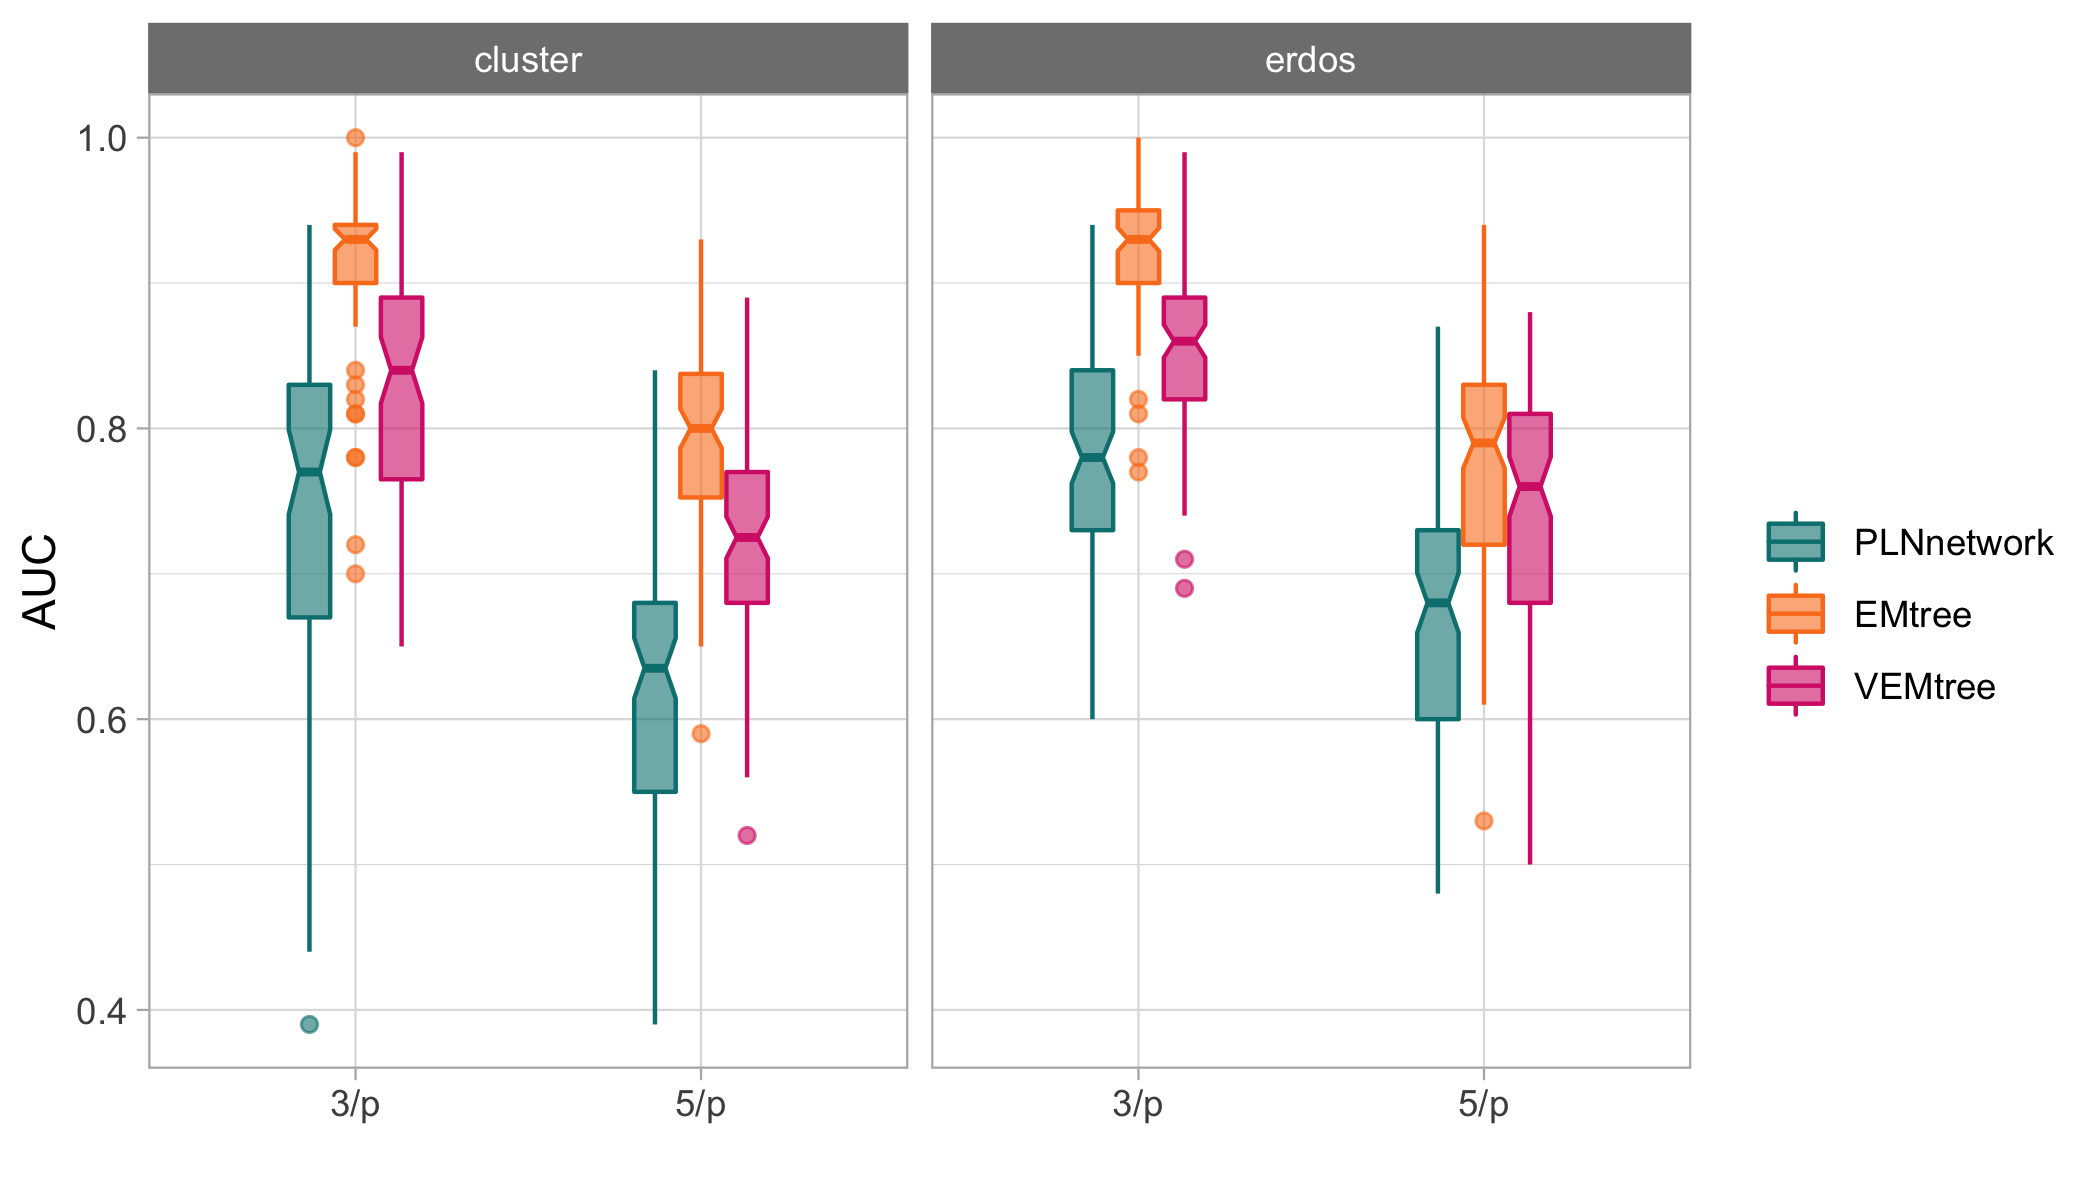
\includegraphics[width=12cm]{figs/AUC_PLN_EM_VEM.png}
\caption{Comparison of PLN-network, EMtree and nestor ability to infer networks with the AUC criteria. 100 datasets were simulated for each parameter settings.}
\label{compar:auc}
\end{figure}
\begin{figure}
\centering
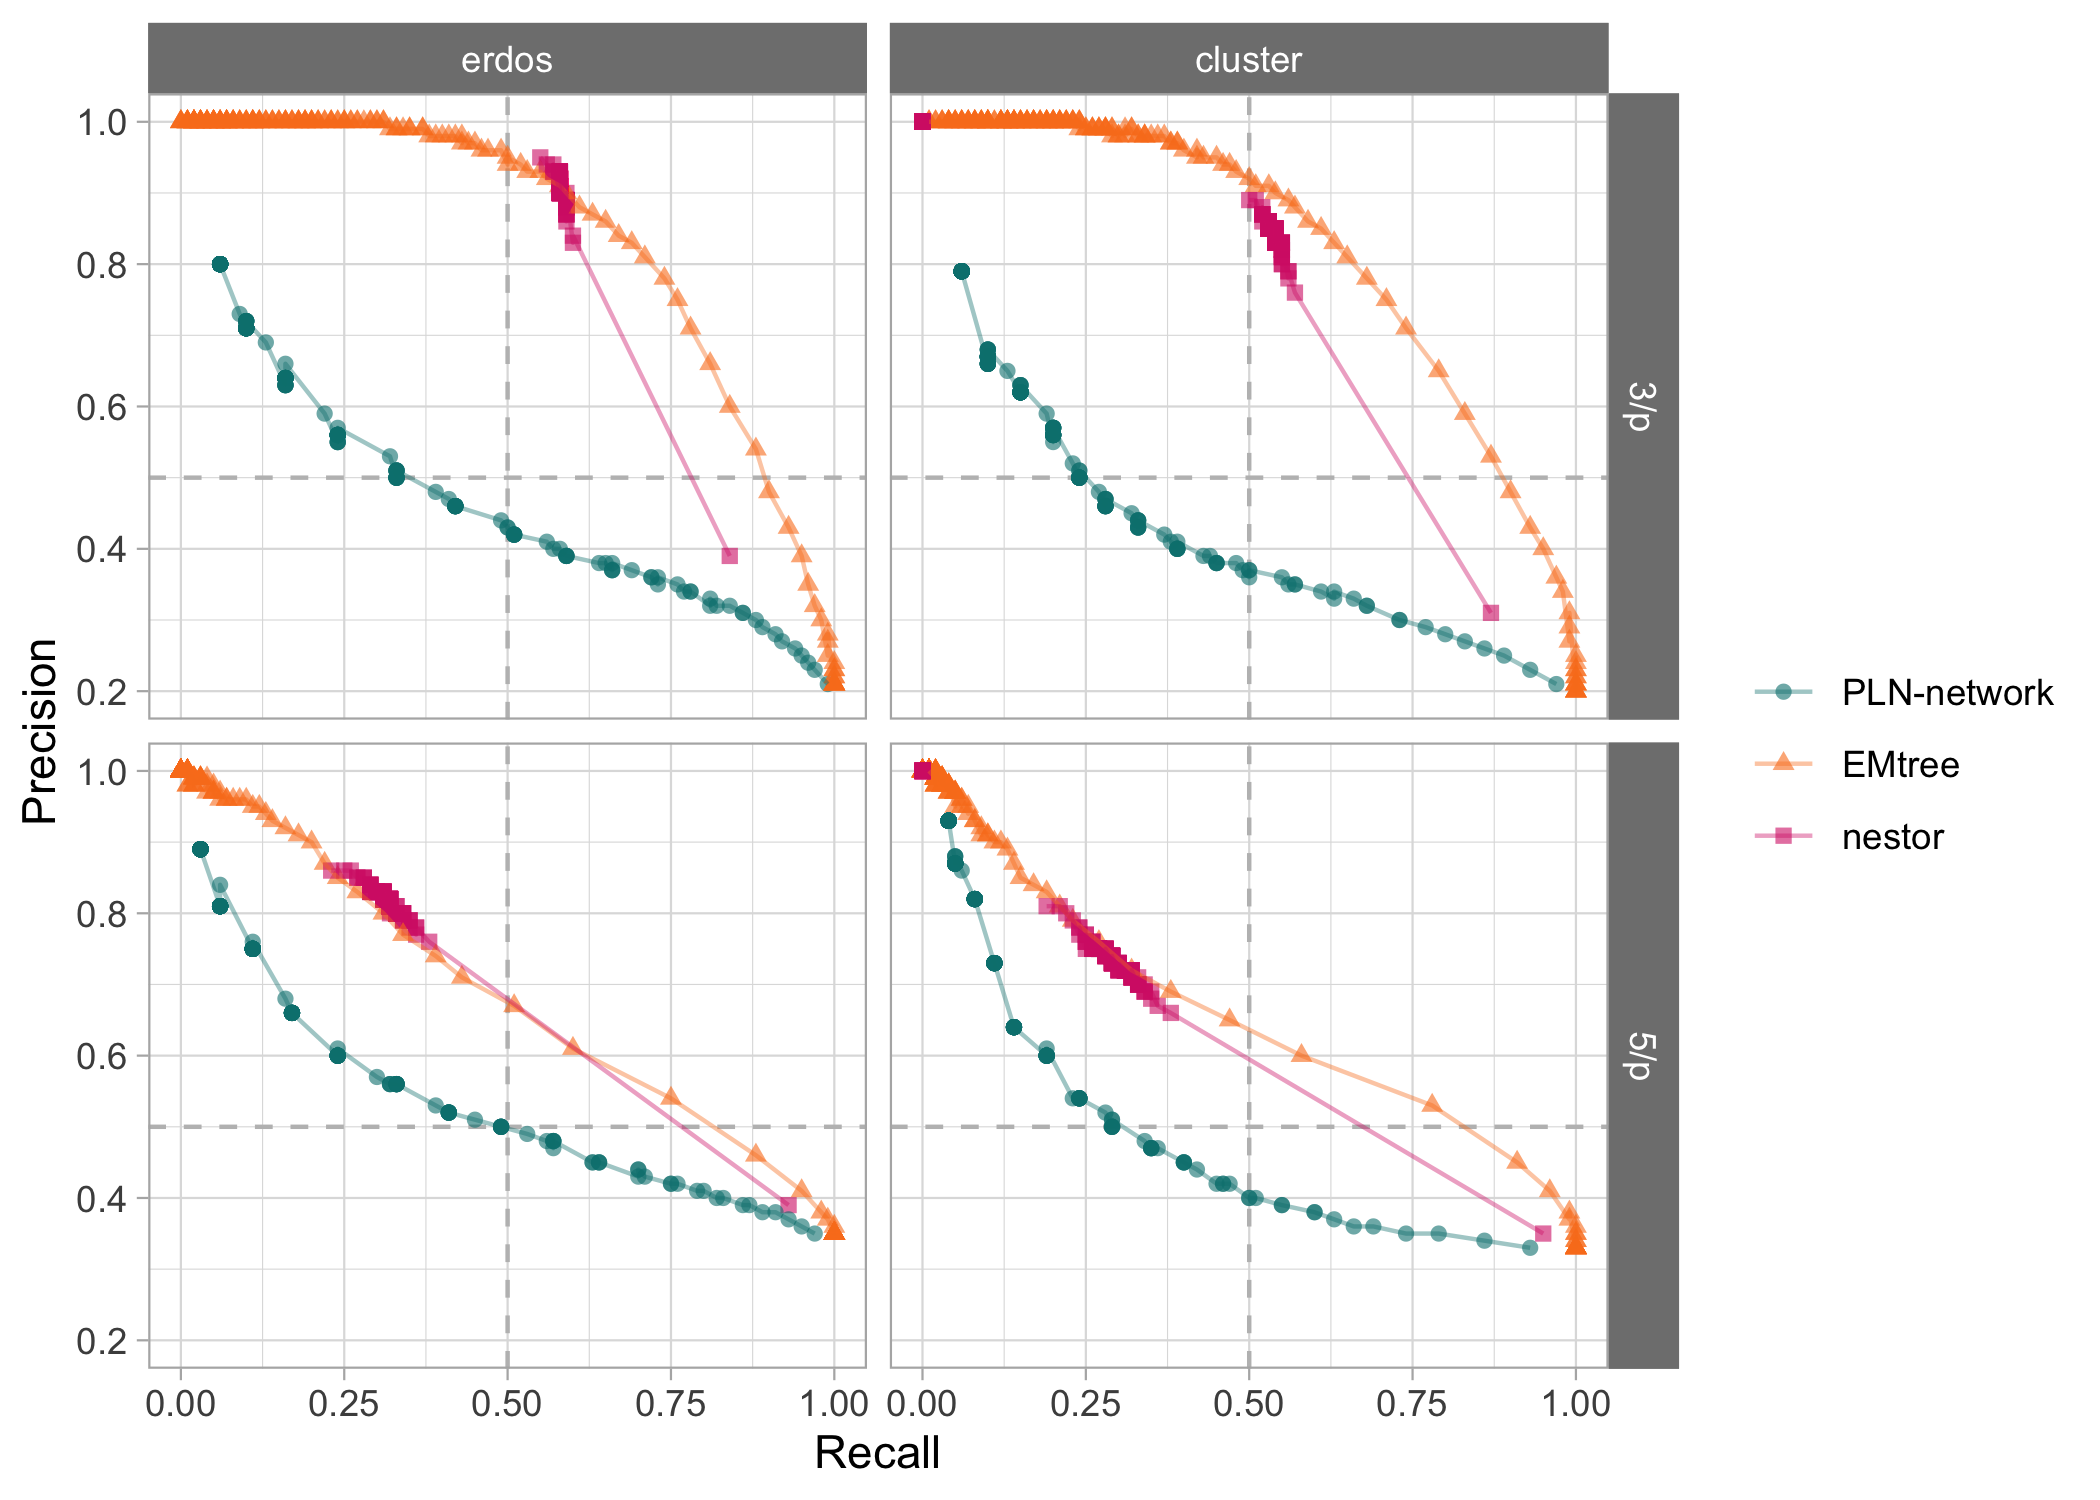
\includegraphics[width=12cm]{figs/precrec_PLN_EM_VEM.png}
\caption{Mean Precision-Recall curves for PLN-network, EMtree and nestor }
\label{compar:precrec}
\end{figure}

with $min.ratio=1\cdot 10^{-3}$ for PLNnetwork
\section{Vignette for nestor}

nestor (Network inference from Species counTs with missingactORs) is an R package for the inference of species interaction networks from their observed abundances, while accounting for possible unobserved missing actors in the data.

\subsection{Simulation and preparation}\label{simulation-and-preparation}

\texttt{nestor} can simulate data with with missing actors with the
function \texttt{missing\_from\_scratch()}. It requires the desired type
of dependency structure (scale-free, erdos, tree or cluster) and the
number of missing actors \texttt{r}. Here is an example with
\texttt{r=1} for the scale-free structure:

\begin{Shaded}
\begin{Highlighting}[]
\KeywordTok{library}\NormalTok{(nestor)}
\NormalTok{p=}\DecValTok{10}
\NormalTok{r=}\DecValTok{1}
\NormalTok{n=}\DecValTok{100}
\NormalTok{data=}\KeywordTok{missing_from_scratch}\NormalTok{(n, p, r,}\DataTypeTok{type=}\StringTok{"scale-free"}\NormalTok{, }\DataTypeTok{plot=}\OtherTok{TRUE}\NormalTok{)}
\end{Highlighting}
\end{Shaded}

\begin{center}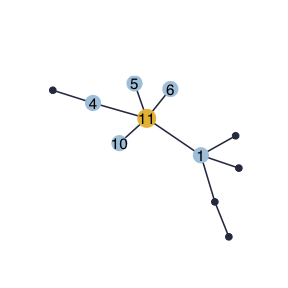
\includegraphics[width=0.3\linewidth]{nestorArticle/man/figures/README-unnamed-chunk-2-1} \end{center}

The original clique of the missing actor neighbors is available in the
value \texttt{TC}:

\begin{Shaded}
\begin{Highlighting}[]
\NormalTok{data}\OperatorTok{\$}\NormalTok{TC}
\CommentTok{#> [[1]]}
\CommentTok{#> [1]  1  4  5  6 10}
\end{Highlighting}
\end{Shaded}

The data is then prepared for analysis with the first step of the
procedure: fit the PLN model. The \texttt{norm\_PLN()} function is a
wraper to \texttt{PLNmodels::PLN()} which normalizes all the necessary
outputs, namely the mean, variance and correlation matrices of the model
latent Gaussian layer corresponding to observed species.

\begin{Shaded}
\begin{Highlighting}[]
\NormalTok{PLNfit<-}\KeywordTok{norm_PLN}\NormalTok{(data}\OperatorTok{\$}\NormalTok{Y)}
\NormalTok{MO<-PLNfit}\OperatorTok{\$}\NormalTok{MO}
\NormalTok{SO<-PLNfit}\OperatorTok{\$}\NormalTok{SO}
\NormalTok{sigma_obs=PLNfit}\OperatorTok{\$}\NormalTok{sigma_obs}
\end{Highlighting}
\end{Shaded}

\subsection{Inference}\label{inference}

\subsubsection{Single clique
initialization}\label{single-clique-initialization}

\texttt{nestor} then needs to be initialized. This requires to find an
initial clique of neighbors for the missing actor, for example using the
\texttt{FitSparsePCA()} function:

\begin{Shaded}
\begin{Highlighting}[]
\NormalTok{initClique =}\StringTok{ }\KeywordTok{FitSparsePCA}\NormalTok{(data}\OperatorTok{\$}\NormalTok{Y,}\DataTypeTok{r=}\DecValTok{1}\NormalTok{, }\DataTypeTok{min.size =} \DecValTok{3}\NormalTok{)}\OperatorTok{\$}\NormalTok{cliques}
\NormalTok{initClique}
\CommentTok{#> [[1]]}
\CommentTok{#> [1]  2  5  7  9 10}
\end{Highlighting}
\end{Shaded}

The \texttt{min.size} parameter defines the minimal size of the output
clique. The function \texttt{init\_mclust()} is also available for
finding a clique, it uses the package \texttt{mclust}.

Once an initial clique has been found, the algorithm can be initialized.
This is the aim of the function \texttt{initVEM()}, which initializes
all required parameters. This function builds one initialization from
one initial clique. We initialize with the clique previously identified:

\begin{Shaded}
\begin{Highlighting}[]
\NormalTok{initList =}\StringTok{ }\KeywordTok{initVEM}\NormalTok{(data}\OperatorTok{\$}\NormalTok{Y, }\DataTypeTok{cliqueList=}\NormalTok{initClique, sigma_obs, MO, }\DataTypeTok{r=}\DecValTok{1}\NormalTok{ )}
\end{Highlighting}
\end{Shaded}

Then to set the tempering parameter \texttt{alpha}, we can look at the
output of the \texttt{alphaMax()} function.

\begin{Shaded}
\begin{Highlighting}[]
\KeywordTok{alphaMax}\NormalTok{(p}\OperatorTok{+}\NormalTok{r, n)}
\CommentTok{#> [1] 0.3000768}
\end{Highlighting}
\end{Shaded}

The actual tempering parameter should be lower than the upper bound
given by \texttt{alphaMax()}. Here we set \texttt{alpha} to \(0.1\). The
core function \texttt{nestor()} can now be run as follows:

\begin{Shaded}
\begin{Highlighting}[]
\NormalTok{fit =}\StringTok{ }\KeywordTok{nestor}\NormalTok{(data}\OperatorTok{\$}\NormalTok{Y, MO,SO, }\DataTypeTok{initList=}\NormalTok{initList, }\DataTypeTok{alpha=}\FloatTok{0.1}\NormalTok{, }\DataTypeTok{eps=}\FloatTok{1e-3}\NormalTok{, }
           \DataTypeTok{maxIter=}\DecValTok{30}\NormalTok{)}
\CommentTok{#> }
\CommentTok{#> nestor ran in 1.078secs and 24 iterations.}
\end{Highlighting}
\end{Shaded}

The object \texttt{fit} contains inferred means and variances of the
complete data, as well as edges weight and probability matrices.

This package contains several visualization functions.
\texttt{plotPerf()} gives a quick overview of the fit performance
compared to initial graph:

\begin{Shaded}
\begin{Highlighting}[]
\KeywordTok{plotPerf}\NormalTok{(fit}\OperatorTok{\$}\NormalTok{Pg, data}\OperatorTok{\$}\NormalTok{G,}\DataTypeTok{r=}\DecValTok{1}\NormalTok{)}
\end{Highlighting}
\end{Shaded}

\begin{center}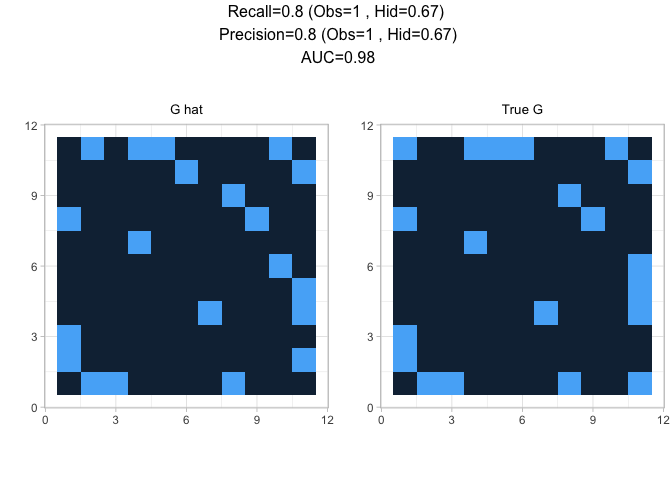
\includegraphics[width=0.8\linewidth]{nestorArticle/man/figures/README-unnamed-chunk-9-1} \end{center}

The convergence of \texttt{nestor()} can be checked with the plotting
function \texttt{plotConv()}:

\begin{Shaded}
\begin{Highlighting}[]
\KeywordTok{plotConv}\NormalTok{(}\DataTypeTok{nestorFit =}\NormalTok{ fit)}
\end{Highlighting}
\end{Shaded}

\begin{center}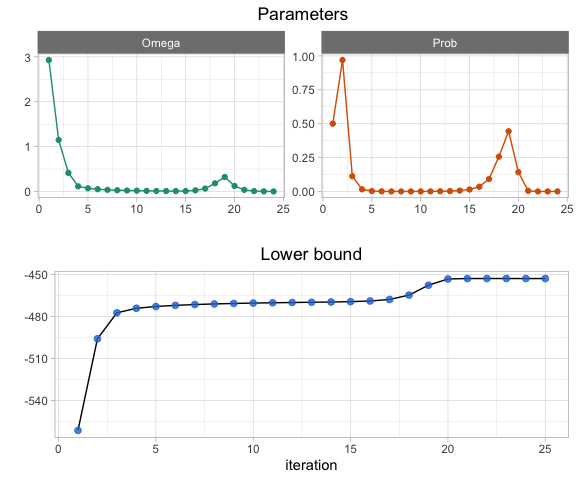
\includegraphics[width=0.8\linewidth]{nestorArticle/man/figures/README-unnamed-chunk-10-1} \end{center}

\subsubsection{Initialization with a list of
cliques}\label{initialization-with-a-list-of-cliques}

The fit of the \texttt{nestor()} function is very sensitive to the
initialization, and so it is recommanded to try several initial cliques.
Several functions are available for finding a list of possible starting
points:

\begin{itemize}
\tightlist
\item
  \texttt{init\_blockmodels()} uses package \texttt{blockmodels},
\item
  \texttt{boot\_FitSparsePCA()} is a bootstraped version using
  \texttt{sparsepca},
\item
  \texttt{complement\_spca()} looks in the complement of the
  \texttt{sparsepca} output.
\end{itemize}

Here we use the \texttt{complement\_spca()} function, which runs
\texttt{sparsepca} and returns the cliques corresponding to the
\texttt{k} first principal components as well as their complement.

\begin{Shaded}
\begin{Highlighting}[]
\NormalTok{six_cliques =}\StringTok{ }\KeywordTok{complement_spca}\NormalTok{(data}\OperatorTok{\$}\NormalTok{Y, }\DataTypeTok{k=}\DecValTok{3}\NormalTok{) }
\NormalTok{six_cliques}
\CommentTok{#> [[1]]}
\CommentTok{#> [[1]][[1]]}
\CommentTok{#> [1] 2 9}
\CommentTok{#> }
\CommentTok{#> [[2]]}
\CommentTok{#> [[2]][[1]]}
\CommentTok{#> [1]  7 10}
\CommentTok{#> }
\CommentTok{#> [[3]]}
\CommentTok{#> [[3]][[1]]}
\CommentTok{#> [1]  2  5 10}
\CommentTok{#> }
\CommentTok{#> [[4]]}
\CommentTok{#> [[4]][[1]]}
\CommentTok{#> [1]  1  3  4  5  6  7  8 10}
\CommentTok{#> }
\CommentTok{#> [[5]]}
\CommentTok{#> [[5]][[1]]}
\CommentTok{#> [1] 1 2 3 4 5 6 8 9}
\CommentTok{#> }
\CommentTok{#> [[6]]}
\CommentTok{#> [[6]][[1]]}
\CommentTok{#> [1] 1 3 4 6 7 8 9}
\end{Highlighting}
\end{Shaded}

This package provides with a parllel procedure for the computation of
several fits of \texttt{nestor()} corresponding to a list of possible
cliques, with the function \texttt{List.nestor()}. Below is an example
with the list of six cliques previously obtained with the
\texttt{complement\_spca()} function:

\begin{Shaded}
\begin{Highlighting}[]
\NormalTok{fitList=}\KeywordTok{List.nestor}\NormalTok{(six_cliques, data}\OperatorTok{\$}\NormalTok{Y, sigma_obs, MO,SO,}\DataTypeTok{r=}\DecValTok{1}\NormalTok{,}
\DataTypeTok{eps=}\FloatTok{1e-3}\NormalTok{,} \DataTypeTok{maxIter =} \DecValTok{50}\NormalTok{, }\DataTypeTok{alpha=}\FloatTok{0.1}\NormalTok{)}
\end{Highlighting}
\end{Shaded}

The object \texttt{fitList} is simply the list of all the
\texttt{nestor()} fits. This procedure aborts in case of degenerated
behaviour, which happens when the provided clique is too far from truth.
Wrong fits can be identified by their ouput size:

\begin{Shaded}
\begin{Highlighting}[]
\KeywordTok{do.call}\NormalTok{(rbind,}\KeywordTok{lapply}\NormalTok{(fitList, length))}
\CommentTok{#>      [,1]}
\CommentTok{#> [1,]    3}
\CommentTok{#> [2,]   12}
\CommentTok{#> [3,]    3}
\CommentTok{#> [4,]   12}
\CommentTok{#> [5,]   12}
\CommentTok{#> [6,]   12}
\end{Highlighting}
\end{Shaded}

Finally we can assess the performance of each converged fit with their
AUC, precision and recall regarding the hidden node \texttt{h}, and the
correlation between the inferred means and the original latent Gaussian
vector of \texttt{h}.

\begin{Shaded}
\begin{Highlighting}[]
\KeywordTok{do.call}\NormalTok{(rbind,}\KeywordTok{lapply}\NormalTok{(fitList, }\ControlFlowTok{function}\NormalTok{(vem)\{}
  \ControlFlowTok{if}\NormalTok{(}\KeywordTok{length}\NormalTok{(vem)}\OperatorTok{>}\DecValTok{4}\NormalTok{)\{}
\NormalTok{    perf=}\KeywordTok{ppvtpr}\NormalTok{(vem}\OperatorTok{\$}\NormalTok{Pg, data}\OperatorTok{\$}\NormalTok{G, }\DataTypeTok{r=}\NormalTok{r)}
    \KeywordTok{c}\NormalTok{(}\DataTypeTok{auc=}\KeywordTok{auc}\NormalTok{(vem}\OperatorTok{\$}\NormalTok{Pg, data}\OperatorTok{\$}\NormalTok{G),}\DataTypeTok{precH=}\NormalTok{perf}\OperatorTok{\$}\NormalTok{PPVH, }\DataTypeTok{recH=}\NormalTok{perf}\OperatorTok{\$}\NormalTok{TPRH, }
    \DataTypeTok{corMH=}\KeywordTok{cor}\NormalTok{(vem}\OperatorTok{\$}\NormalTok{M[,p}\OperatorTok{+}\NormalTok{r], data}\OperatorTok{\$}\NormalTok{UH))}
\NormalTok{  \}}
\NormalTok{\})) }\OperatorTok\StringTok{ }\KeywordTok{as_tibble}\NormalTok{()  }
\CommentTok{#> # A tibble: 4 x 4}
\CommentTok{#>     auc precH  recH  corMH}
\CommentTok{#>   <dbl> <dbl> <dbl>  <dbl>}
\CommentTok{#> 1  0.81  0.6   0.5  -0.785}
\CommentTok{#> 2  0.93  0.75  1    -0.815}
\CommentTok{#> 3  0.76  0.5   0.67 -0.715}
\CommentTok{#> 4  0.69  0.43  0.5  -0.585}
\end{Highlighting}
\end{Shaded}


 
\end{subappendices}

%\clearemptydoublepage
%\addtocontents{toc}{\protect\newpage}
\chapter{Perspectives}

 \vspace{0.5cm}
 
 The previous chapters detailed the proposed methodology for network inference from incomplete abundance data. The species abundances $\Ybf$ are jointly modeled in a GLMM using the Poisson log-normal distribution, thus taking advantage of its properties to account for offsets and experimental and/or environmental covariates $\Xbf$. The problem of network inference is then transposed to the Gaussian latent layer of model parameters $\Zbf$, where it is performed using averaging on spanning-tree structures with decomposable distribution on trees parametrized with edges weights $\betabf$. Missing actors are inferred in the Gaussian layer as well, simultaneously with the network. We remind the mathematical formulation of this model:
  \begin{equation*}
 \left\{ \begin{array}{l}
 \begin{array}{ll}
 T\sim \prod_{kl\in T} \beta_{kl} / B, &B= \sum_{T\in\mathcal{T}} \prod_{kl \in T} \beta_{kl},\\\\
 \Zbf_i\mid T  \sim \Ncal (0, \Omegab_T), &\{\Zbf_i\}_i \text{ iid, }\\
 \end{array} \\\\
 Y_{ij}\mid \Zbf_i\sim \Pcal (\exp (o_{ij}+\xb_i^\intercal \thetab_j + Z_{ij})), \; (Y_{ij} \independent) \mid \Zbf_i 
 \end{array} \right. .
 \end{equation*}
 
 The qualities of this approach have been demonstrated on simulated examples as well as empirical datasets. But why does it work ? Mostly because exact computations are possible in the Gaussian layer, thanks to its maniability and the structure and algebraic properties of spanning trees.  This flexibility calls for some natural extensions which were not developed due to time constraints, that we now present together with specific details of this model.
 
 
\section{Unresolved questions}
\subsubsection*{Offset modeling}
The presented methodology allows to take into account covariates and offsets, which is paramount in the modeling of experiments. A change in the covariates included can greatly modify the inferred network, however this is an information that can be controlled. On the other hand, not including offsets amounts to model incoherent data and therefore yields inconsistent results. Unfortunately, offsets are not always obvious or easy to get, and evaluating them possibly represents a modeling step in itself. For example in an ecological census of fauna, the offset has to at least account for the period of time of observation, the experience of the observer and the species detectability, which is obviously the most difficult to get. Detectability depends on the relative position of the species to the observer, and can depend on the environmental conditions as well, making its modeling a delicate step.\\

\subsubsection*{Algorithm initialization}
The approach can also infer missing actors as detailed in Chapter 3. The initialization of the algorithm for this inference requires an initial clique of neighbors for each missing actor. This parameter is critical, as it defines all the initialization and if it is too far from the true clique, that is if not a minimum of true neighbors are included, the procedure can degenerate and abort. Several methods for setting this parameter are proposed in the nestor package. They are based on finding groups of highly correlated variables (sparse PCA and model-based clustering of the estimated correlation matrix), or finding clusters in the structure of the marginal graph (using Stochastic Bloc Models). The estimated lower bound of the likelihood can be used to choose between a large set of results with different initializations, thus one way to go is simply to sample several starting points (possibly by boostrapping the previous methods) and test all of them. Many other methods could be used, as well as prior knowledge on species, and we do not conclude on the best way to initialize the cliques. However we observed that it is less important for the inference quality to be precise than to include some true neighbors in the clique. Therefore we advise to choose the initial clique also based on its size.\\

\subsubsection*{Model selection}
One key question when working with possibly incomplete data is to know if it is indeed incomplete, and to what extent. This amounts to model selection to chose the number of missing actors $r$.  Usually model selection is carried out with computations on the likelihood of each model. The model developed involves several latent parameters, and the inference is therefore performed in a variational framework which yields a lower bound of the likelihood. Moreover as the method takes advantage of the variational estimation of the PLN model described in \citet{CMR18}, the quantity that is computed is actually an approximation of this lower bound. This results in the usual model selection tools, which originally apply to likelihoods, to not work (Akaike/Bayesian/Extended Bayesian Information Criterion). Then the only strategy left is to resort to cross-validation, which is greedy and not very satisfying either. There is a need of  adapted criteria for  models with variational inference, which is still an open research question of statistical theory.

\section{Extensions of the adopted approach}
In this section, we present direct extensions of the developed methodology regarding the network in itself (estimation of its parameters, network comparison), and the data nature (processing of different data types and spatialized data).
\subsection{Characterizing species interactions}


Generally, species interactions are characterized by their sign and strength. This information is contained in  the partial correlation matrix, defined as $\Rbf_p=(\rho_{jk})_{1\leq j,k\leq p}$ with $$\rho_{jk}=\frac{-\omega_{jk}}{\sqrt{\omega_{jj}\omega_{kk}}},$$
 which is simply the opposite of the correlation matrix built from the precision matrix $\Omegabf$. Some methods are thus dedicated to the estimation of the partial correlation matrix to build knowledge on an ecosystem functioning. In the context of Gaussian Graphical Models, \cite{Lau96} develops maximum likelihood estimators for the precision matrix which depends on that of the covariance matrix, and the structure of the graph, as detailed in section \ref{ggm:mle}. It thus requires the precise knowledge of the graph, and even more than that: the only terms of the covariance matrix that are correctly estimated are those corresponding to edges in the graph. Therefore the prior inference of the structure is necessary. Moreover, these MLE are only valid for decomposable graphs, therefore using Proposition \ref{decomp} the network might need to be triangularized as illustrated in Figure \ref{chordal}. Therefore following these three steps: 
\begin{enumerate}
\item Infer the conditional dependency structure $\G$,
\item Make $\G$ a chordal graph,
\item Compute $\widehat{\Omegabf}_{MLE}$.
\end{enumerate}
 would lead to an approximation of $\Omegabf$. Note that there is not a unique solution to step 2.  If the inferred network is already chordal, this  yields  the MLE of $\Omegabf$, available after the network inference.

\begin{figure}
\centering
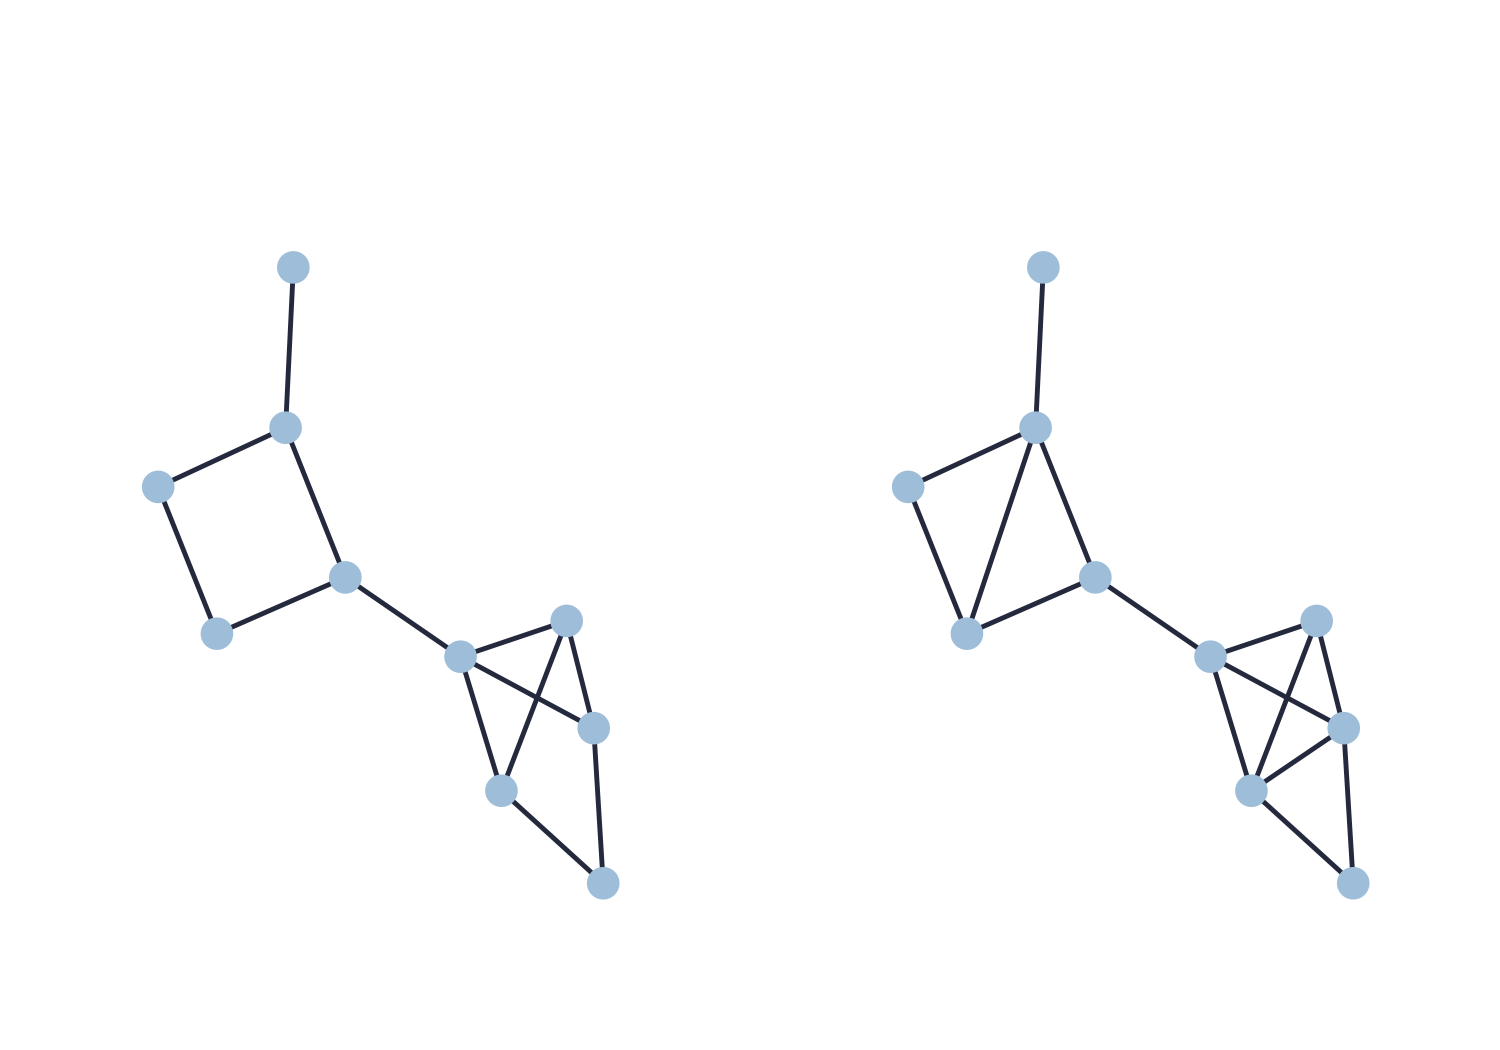
\includegraphics[width = 0.6\linewidth]{figs/chordal.png}
\caption{Example of triangularization. \textit{Left}:  graph $\G$. \textit{Right}: a chordal version of $\G$: maximal loops are of size 3.}
\label{chordal}
\end{figure}
\subsection{Network comparison}
 
Comparing networks has many applications and  yields results of interest in various fields, regarding for example the evolution of a system across seasons, or how a pathogen modifies the organization of a microbiome.

The comparison from a statistical point of view is linked to testing differences, or questioning the independence of two networks for example.  Rather than defining statistical tests based on networks distributions, current strategies consists in summarizing networks with vectors of measures on nodes. These are called embeddings, which aim to capture the structure of the graph and the relationships between the nodes in a concise manner (e.g. \citet{TMK18,CK19}). Embeddings can then be compared using PCA for example. The presented approach assumes the graph is a latent tree, which estimated distribution can be seen as another available graph summary.\\

A first step toward statistical network comparison using trees could be to compare the estimated laws on trees, for example using the Küllback-Leibler divergence which is easily written with tree distributions and gives two interesting quantities.

First, it is possible to compute the contribution of a specific edge $kl$ to the distribution. We denote $p_{\betabf_{\setminus kl}}$ the  decomposable tree distribution where the weight $\beta_{kl}$ is set to zero. Its normalization constant is  $B_{\setminus kl}=\sum_{T\in\mathcal{T}} \prod_{uv\neq kl} \beta_{uv}$. Computing the Küllback-Leibler divergence between $p_\betabf$ and $p_{\betabf_{\setminus kl}}$ yields  the contribution of $kl$ to $p_\betabf(T)$. It writes:
\begin{align*}
KL( p_\betabf (T)\mid\mid p_{\betabf_{\setminus kl}} (T)) &= \Esp_{p_\betabf (T)} [\log p_\betabf (T) - \log p_{\betabf_{\setminus kl}} (T)]\\
&=P_{kl} \log \beta_{kl} + \log ( B_{\setminus kl}/B).
\end{align*}
Where $P_{kl} = \Esp_{p_{\betabf}}[\mathds{1}\{kl\in T\}]$ is the probability for the edge $kl$ to be in tree $T$ under the tree distribution $P_{\betabf}$. Now noticing that $B_{\setminus kl}/B=1-P_{kl}$, we finally get the following contribution of $kl$:
$$KL( p_\betabf (T)\mid\mid p_{\betabf_{\setminus kl}} (T)) =P_{kl} \log \beta_{kl} + \log (1-P_{kl}).$$
%peut être utile pour ordonner les arêtes par importance si trop de probabilités égales. Besoin de faire un test pour voir si la qté existe 	vec une proba à 1 (existance de B\kl)
As the distribution under which the expectation is taken must be dominant over the other, the divergence $KL(p_{\betabf_{\setminus kl}} (T)\mid\mid p_\betabf (T)) $ is not defined.

Then, if all edges weights are finite and non-null, the divergence can be symmetrized into a so-called dissimilarity measure to compare two networks. Assuming the data is observed under two conditions $A$ and $B$, we consider the edges weights matrices estimated from each subsets $\betabf^A$ and $\betabf^B$. The dissimilarity measure between the tree distributions  $p_{\betabf^A}(T)$ and $p_{\betabf^B}(T)$ writes:
\begin{align*}
D(p_{\betabf^A}(T), p_{\betabf^B}(T)) &=\frac{1}{2} \left[KL\big( p_{\betabf^B} (T) \mid\mid p_{\betabf^A}(T)\big)+KL\big( p_{\betabf^A}(T)\mid\mid p_{\betabf^B} (T)  \big)\right].
\end{align*}
After computation, this actually simplifies into the following expression, where $P_{kl}^A = \Esp_{p_{\betabf^A}}[\mathds{1}\{kl\in T\}]$ is the probability for the edge $kl$ to be in tree $T$ under the tree distribution $p_{\betabf^A}$:
$$D(p_{\betabf^A}(T), p_{\betabf^B}(T)) = \sum_{kl} \log (\beta_{kl}^A /\beta_{kl}^B) \left( \frac{P_{kl}^A - P_{kl}^B}{2}\right).$$

Finally if we consider $K$ different conditions,  the $K$ tree distributions could be compared by computing the $K\times K$ matrix of dissimilarity measures, provided that all edges weights are finite and non-null.
%(si temps pour exemple, MDS 2 premiers axes)

\subsection{Other data types}
This work focuses on abundance data, however the network inference method developed here could be extended to other data types. Indeed, the strategy of tree averaging is based on the Gaussian Layer of the $\Zbf$. Therefore it could also be used with a model which would keep this layer and add a different emission law than the Poisson to generate data $\Ybf$, that is considering the model 
  \begin{equation*}
 \left\{ \begin{array}{l}
 \begin{array}{ll}
 T\sim \prod_{kl\in T} \beta_{kl} / B, &B= \sum_{T\in\mathcal{T}} \prod_{kl \in T} \beta_{kl},\\\\
 \Zbf_i\mid T  \sim \Ncal (0, \Omegab_T), &\{\Zbf_i\}_i \text{ iid, }\\
 \end{array} \\\\
 Y_{ij}\mid \Zbf_i\sim F (o_{ij},\xb_i,Z_{ij}), \; (Y_{ij} \independent) \mid \Zbf_i 
 \end{array} \right. .
 \end{equation*}
For example, choosing the emission law $F$ as  binomial, multinomial or a Tweedie distribution \citep{T84} would respectively yield presence/absence, ordinal, or positive continuous data (e.g. to model biomass). Mixed data could also be generated, as long as the emission law parameters are stored in the Gaussian layer $\Zbf$. 

Another interesting extension is for $F$ to be multidimensional.  Nodes of the network would then be vectors of information known as multi-attribute variables. This can be the case when multiple measures on the same system are available. For example in microbiology, different information can be measured on a set of genes such as transcriptomics, proteomics, or metabolomics data. Then these multiple sources can be integrated to infer the gene regulatory network \citep{CRS19,SFC19}.  

Choosing another emission law  would require to estimate its parameters, which can be a sensitive task. However the network inference mechanics in the Gaussian layer using tree averaging would remain the same. 

\subsection{Spatial dependence}
In ecological surveys, environmental conditions might be spatially heterogeneous (e.g. different climate at different altitudes).   This translates in spatial correlation in the observed data, which has to be accounted for in the network inference.

Spatial correlation is due to spatially close environments being similar. Therefore a first and quick way to correct for spatial dependence is to include environmental covariates encoding the spatial proximity (e.g. spatial coordinates) in the model. For example Figure \ref{vario} shows how a variogram may be flattened by adjusting for latitude and longitude.
\begin{figure}
\centering
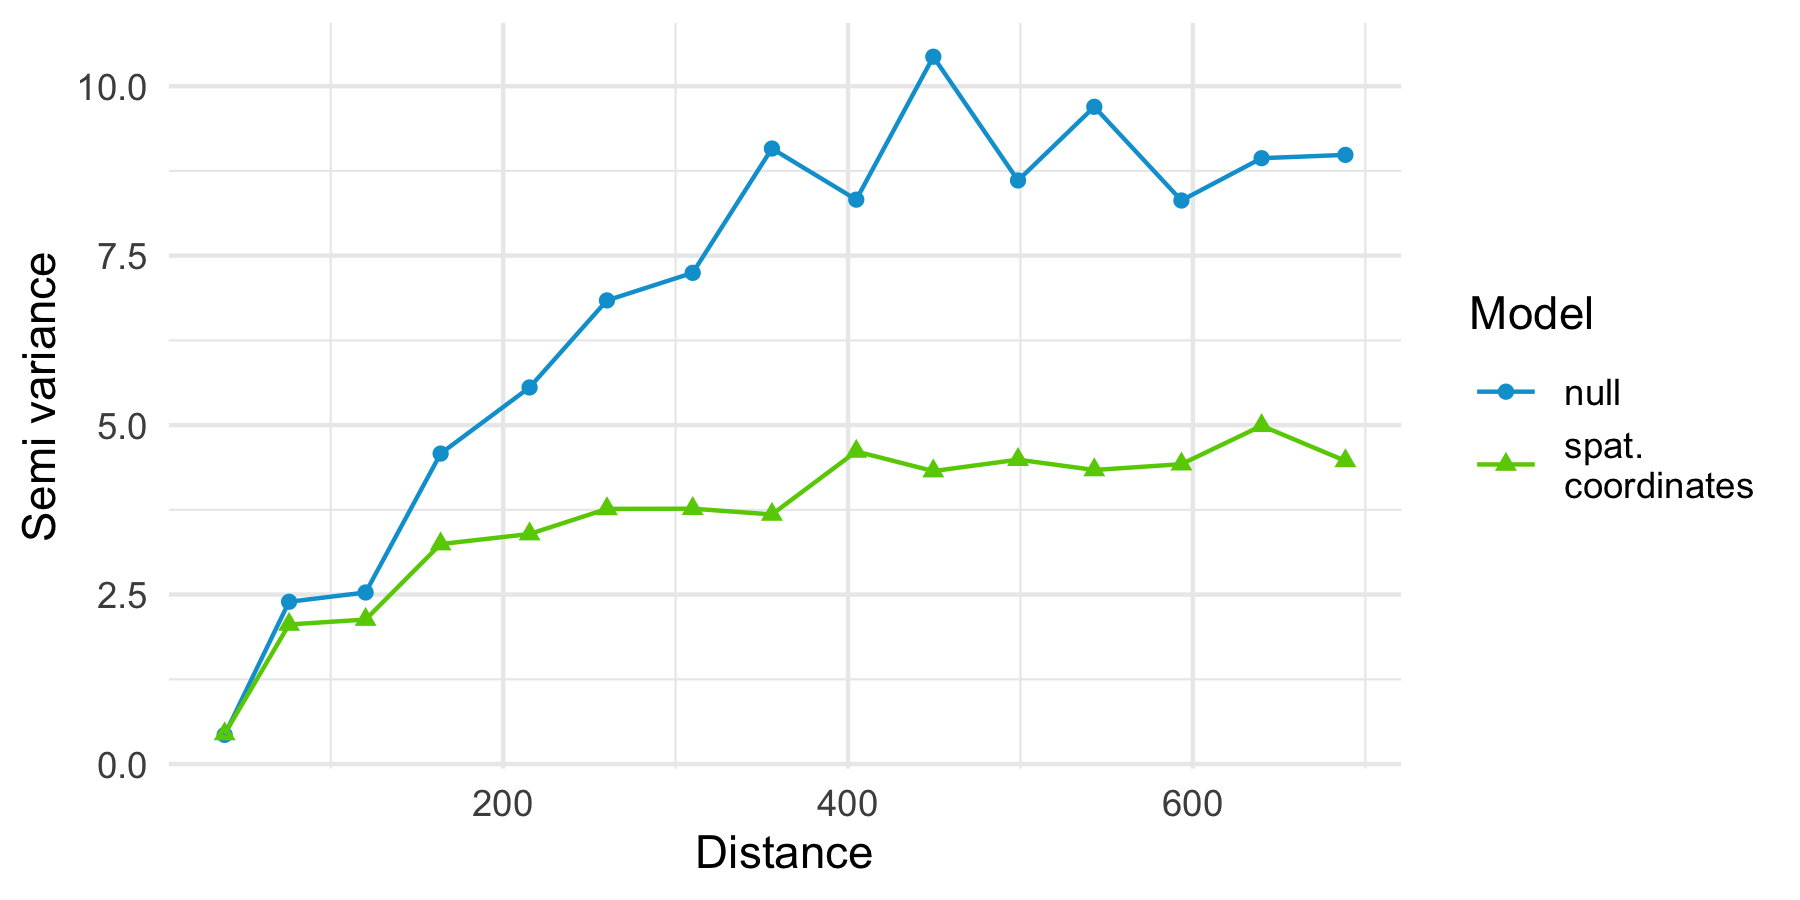
\includegraphics[width=10cm]{figs/variogram.png}
\caption{Variogram of the species Trisopterus esmarkii (Norway pout) from the Barents dataset with and without adjusting linearly for the spatial coordinates.}
\label{vario}
\end{figure}
However such correction might not be enough and the residuals from the adjustment might still be spatially correlated. Spatial coordinates could be adjusted in a more complicated way than the linear relationship, but another solution is to consider this dependence to be the result of an unobserved variable. As a missing variable, the spatial dependency can be taken into account to unravel the direct dependencies among species by using the method detailed in Chapter 3. Adjusting for spatial covariates corrects for the spatial effects on the means, whereas including spatial dependence  as a node in the interaction network corresponds to a correction of the variances.

%These two solutions aim at correcting for the spatial effect, which is thus considered as a kind of noise on the signal of species dependencies. However, one might be interested in modeling this spatial effect for further study. 

Another way of correcting the variances for spatial dependencies is to include spatial variances directly in the model. To do this a first approach is to assume a separation of the dependencies due to the spatial effects stored in the matrix $\Gamma=(\Gamma_{st})_{1\leq s,t\leq n}$ on the one hand, and due to the species interactions stored in the matrix $\Sigma=(\sigma_{jk})_{1\leq j,k\leq p}$ on the other hand. To simplify we consider either pairs of species $j$ and $k$ on the same site $s$ or a same species $j$ on pair of sites $s$ and $t$. The Gaussian parameters are then modeled as follows:
\begin{align*}
(Z_{sj},Z_{sk}) &\sim \Ncal(0, \gamma_{ss} \Sigma_{[j,k]}),\\
(Z_{sj},Z_{tj}) &\sim \Ncal(0, \sigma_{jj} \Gamma_{[s,t]}).
\end{align*}

That way we obtain $\Cov{(Z_{sj},Z_{sk})} = \gamma_{ss} \sigma_{jk}$ and $\Cov{(Z_{sj},Z_{tj})} =  \sigma_{jj}\gamma_{st}$. This is equivalent to consider the transformation of the matrix $\Zbf$ into the vector $Vec(\Zbf) = (Z_{11},..., Z_{1p},Z_{21},...,Z_{np}) \in \mathds{R}^{n\times p}$ to be distributed as:
$$Vec(\Zbf) \sim \Ncal(0,\Gamma \otimes \Sigma).$$ 

As the covariance structure is different for a pair of sites or a pair of species, this model requires to use the bivariate Poisson log-normal distribution for the count data $\Ybf$.
It is then be possible to write a pairwise composite log-likelihood which involves all the variance parameters:
$$c\ell_\theta(\Ybf) = \sum_{j=1}^p \sum_{s<t} \log p_\theta(Y_{sj}, Y_{tj})+\sum_{s=1}^n \sum_{j<k} \log p_\theta(Y_{sj}, Y_{sj}).$$

The number of parameters for the variance is $\frac{1}{2}(n^2+ p^2)$, which is quite large. Classically to reduce this number, the $\Gamma$ matrix is parametrized with a spatial covariance function.  For example the Matérn functions (which include the exponential covariance function and others) define the covariance between two points distant of $d$ units from each other as a function of $d$ and three other parameters \citep{CW15}.

Performing network inference using tree averaging in this case would simply amount to consider 
$$Vec(\Zbf) \sim \Ncal(0,\Gamma \otimes \Sigma_T),$$
then the inference of edges probabilities would go as previously detailed.
 
%ovaskainen hmsc fait le job, à vérifier

\section{Network inference in the observed layer}
All of the above is an adaptation of the presented model to perform network inference in the latent Gaussian layer of parameters.
 However it can be shown that if the graphical model in the latent Gaussian layer $\Zbf$ is a connected graph, then the marginal graphical model of the observed counts $\Ybf$ is a clique. 
\begin{figure}[H]
\centering
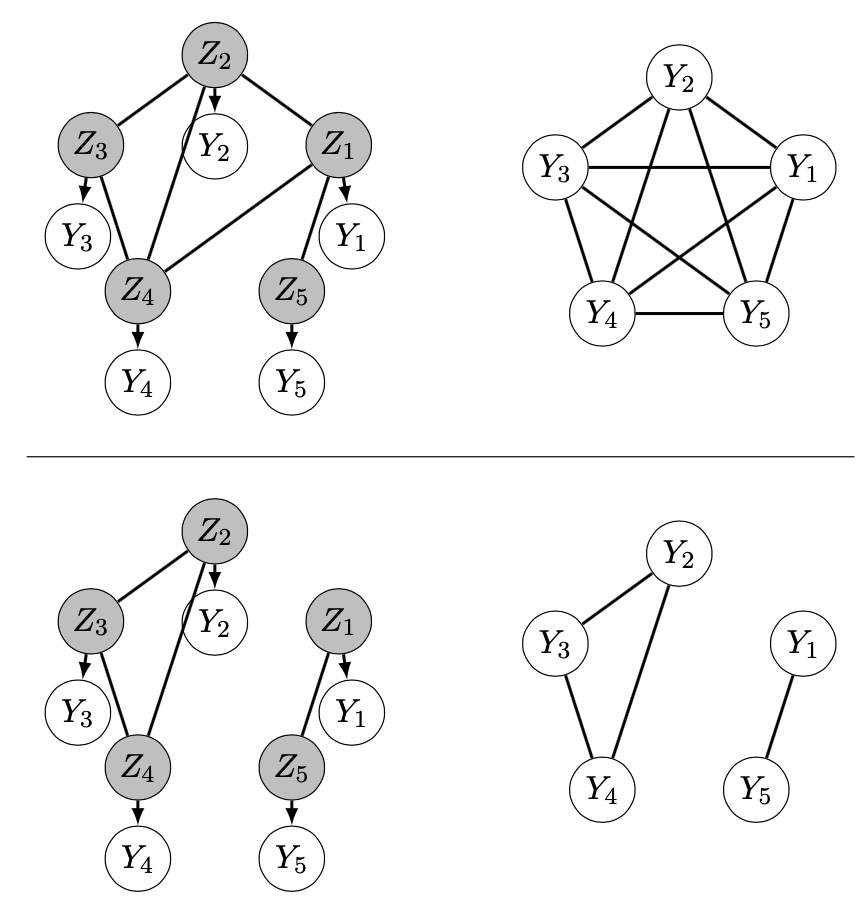
\includegraphics[width=0.5\linewidth]{figs/YZ.png}
\caption{Graphical representation of the joint distribution $p(Z_i,Y_i)$ (left) and marginal distribution $p(Y_i)$ (right) when the graphical model of the latent variables is connected (top) or not (bottom).}
\label{YZ}
\end{figure}
As Figure \ref{YZ} illustrates, only a separation in the latent space results in a separation in the observed space.


It is possible to write a model which meets the primary goal of inferring  the network directly in the space of observed data $\Ybf$. Considering any marginal and bivariate discrete distribution for counts, assuming a tree-shaped dependency structure for the counts writes: %it is possible to write the following model for the network inference using tree averaging:

 $$p_\theta(\Ybf_i \mid T) = \prod_{j=1}^p p_\theta(Y_{ij}) \prod_{jk\in T} \frac{p_\theta(Y_{ij},Y_{ik})}{p_\theta(Y_{ij})p_\theta(Y_{ik})}.$$
 
Covariates and offsets could be involved as parameters on the distributions means. Then the joint distribution of counts would be a mixture on trees:
$$p_{\beta, \theta}(\Ybf ) = \sum_{T\in \mathcal{T}} p_\beta(T)p_\theta(\Ybf\mid T).$$

This model involves only one latent layer: the tree $T$. With a decomposable distribution on $T$, the quantity $\Esp_{\beta, \theta}[\log p_{\beta, \theta}(\Ybf, T)\mid\Ybf]$ of the E step of an EM algorithm could be estimated using the Matrix Tree Theorem. Regarding the M step, the estimation of the weights $\beta$  would be the same as for the PLN model with network inference in the Gaussian layer. However the estimation of the $\theta$ parameter is complex, as its estimator is usually not explicit and is common to several terms of the product on the edges in $p_\theta(\Ybf\mid T)$. The M step is thus the main difficulty for the estimation of this model.



%\selectlanguage{french}
\clearemptydoublepage
\DeactivateBG 
\chapter{Résumé}
\textit{This chapter is a summary of the present work, written in French.}\\

Les réseaux sont des objets qui permettent de graphiquement représenter des liens entre des entités.  Ces outils sont utilisés dans des domaines très variés, allant de l'informatique aux neurosciences, aux sciences sociales et à la biologie. Ce travail s'intéresse aux réseaux d'espèces en écologie et microbiologie (ou méta-génomique), et plus particulièrement à l'inférence des réseaux de dépendances conditionnelles entre espèces d'une même communauté partageant le même environnement. Les réseaux représentent alors les espèces par des noeuds, et leurs liens de dépendances par des arêtes.

 L'inférence de réseau considérée ici a pour point de départ des mesures répétées de comptages des espèces d'intérêt, soit un tableau de données de $n$ mesures discrètes de $p$ espèces. Il est important de distinguer ce cas de figure où le réseau n'est pas connu ni observé, de celui où il est possible d'observer les liens du réseau directement, et donc de reconstruire ce dernier via des comptages d'interactions observées, comme c'est classiquement le cas en écologie par exemple. Considérer les relations de dépendances conditionnelles permet à la fois d'obtenir des réseaux parcimonieux et interprétables en ne représentant que des liens directs entre espèces, et d'inférer des liens qui ne sont pas directement observables comme par exemple les dépendances entre des (pseudo-)espèces microscopiques (bactéries, champignons, protéines, virus, gènes, etc.) ou des liens dont la nature les rend difficilement identifiables (par exemple les relations de coopération ou de communication). \\

Les modèles graphiques sont le cadre mathématique des réseaux de dépendances conditionnelles.  Notamment, les modèles graphique gaussiens possèdent des propriétés particulières facilitant leur inférence. Ce cas particulier est un cadre très utilisé pour l'inférence de réseaux en biologie, cependant il n'est pas directement applicable à des données discrètes.  Le premier objectif de ce travail est ainsi de développer une méthodologie pour l'inférence de réseaux de dépendances conditionnelles à partir de données de comptages. Par ailleurs, pour assurer la validité des résultats il est nécessaire que les covariables expérimentales ainsi que les offsets mesurés (durées d'observation, profondeur de séquençage) soient inclus dans la modélisation des comptages. L'inférence de réseau en elle-même tire parti des propriétés algébriques des arbres couvrants pour réaliser une exploration efficace et exhaustive de l'espace des graphes réduit à celui de ces structures particulières.


Il est en outre possible que toutes les espèces ou covariables n'aient pas été mesurées lors de l'expérience. Un réseau inféré à partir de données incomplètes est alors un réseau marginal, qui présente mécaniquement des formations denses entre les espèces liées à un acteur non observé menant à des interprétations biaisées et partielles. Le second objectif de ce travail est  d'inclure de possibles acteurs manquants dans l'inférence, afin d'obtenir à la fois le réseau complet et des informations permettant de caractériser et de mieux comprendre les acteurs manquants. 


\section*{Chapitre 1}
Le premier chapitre  expose en détails les éléments de théorie invoqués pour la modélisation et l'inférence développées dans les chapitres suivants. Le cadre des modèles graphiques est tout d'abord abordé de manière générale et inspirée de \citet{Lau96}, avant d'introduire les arbres couvrants et leurs propriétés algébriques. Dans un second temps, les particularités des modèles graphiques gaussiens sont présentées, anisi que deux méthodes pour leur inférence. Après un bref exposé de l'inférence dans le cadre de données incomplètes, la dernière partie traite de l'inférence de réseaux à partir de données de comptage et présente plusieurs stratégies issues de la littérature en écologie des communautés et microbiologie.

\subsection*{Modèles graphiques}
\subsubsection*{Définitions générales.}
Un graphe $\G$ est constitué d'un ensemble de noeuds $V$ et d'un ensemble d'arêtes $E$. Pour un triplet $(A, B, S)$ de sous-ensembles disjoints de $V$, l'ensemble $S$ sépare $A$ et $B$ dans $\G$ si tout chemin allant de $A$ à $B$ intersecte $S$. La notion de séparation est essentielle  pour établir le lien entre graphe et relations d'indépendances conditionnelles au sein d'une variable aléatoire multi-variée. 

Soit $\G$ un graphe non-dirigé et $X=(X_v)_{v\in V}$ un vecteur aléatoire à valeurs dans un espace produit $\mathcal{X}=\otimes_{v\in V} \mathcal{X}_v$. Pour tout sous-ensemble $A$ de $V$, $X_A$ dénote $(X_v)_{v\in A}$.


\textbf{Propriété} (Markov globale). \textit{Une mesure de probabilité sur $\mathcal{X}$ satisfait la propriété de Markov globale  par rapport à $\G$ si pour tout triplet $(A, B, S)$ de sous-ensembles disjoints de $V$, on a
$$\text{S sépare A et B } \Rightarrow X_A\independent X_B \mid X_S.$$ }
Un modèle graphique pour $X$ est alors tout graphe tel que la distribution de $X$ soit globale Markov par rapport à ce graphe. La propriété de Markov globale est seulement une implication, ce qui signifie qu'il est autorisé qu'un modèle graphique n'inclue pas toutes les relations d'indépendances conditionnelles. Lorsque que la relation est une équivalence, la distribution de $X$ est dite fidèle Markov, et le graphe associé représente exactement toutes les relations d'indépendances conditionnelles dans $X$.


Si $S$ sépare $A$ et $B$ et si de plus tous les noeuds dans $S$ sont liés enter eux ($S$ est complet), le triplet $(A,B,S)$ est alors une décomposition propre de $\G$. Cette notion permet de définir un graphe décomposable.


\textbf{Définition} (Graphe décomposable). \textit{Un graphe $\G$ est dit décomposable s'il existe une décomposition propre $(A, B, C)$ sur $\G$, et si les sous-graphes définis par $A\cup B$ et $B\cup C$ sont eux-mêmes décomposables.}


Les modèles graphiques à graphes décomposables permettent de structurer l'écriture des paramètres de variance sur des ensembles de variables complets, ce qui facilite leur estimation. 

\subsubsection*{Arbres couvrants.}
Parmi l'ensemble des graphes, les arbres couvrants sont les structures les plus parcimonieuses, et les structures sans cycles les plus denses. Naturellement décomposables, ils sont pratiques à manipuler grâce à leurs propriétés algébriques. L'espace des graphes non-dirigés est de taille super-exponentielle ($2^{p(p-1)/2}$ graphes possibles pour $p$ noeuds). L'espace des arbres couvrants, bien que plus petit, reste combinatoirement grand ($p^{p-2}$ arbres pour $p$ noeuds). Il est cependant possible de sommer sur cet espace en $\mathcal{O}(p^3)$ opérations. Ce théorème est l'extension aux réels du théorème de Kirchhoff  \citep{matrixtree, MeilaJaak}, connu sous le nom de théorème arbre-matrice ou des mineurs égaux. \\


\textbf{Théorème} (Arbre-matrice). \textit{Soit une matrice de poids symétrique $\Wbf=(w_{jk})_{jk}$ dont les entrées sont dans $\mathds{R}^+$. Alors la somme sur l'ensemble des arbres couvrants du produit des poids de leurs arêtes est égal à n'importe quel mineur du Laplacien $\Qbf$ de $\Wbf$. Formellement, pour tout $1 \leq u, v \leq p$ :
   \[  W := \sum_{T\in\mathcal{T}} \prod_{jk\in T} w_{jk} = |\Qbf^{uv}|.  \]
   }
   
Ce théorème fait apparaître une forme somme-produit sur l'espace des arbres couvrants. Le lemme technique qui suit, établi par \citet{MeilaJaak}, permet de dériver une telle somme. On rappelle que le Laplacien d'une matrice est la matrice dont les termes diagonaux (resp. extra-diagonaux) sont les sommes par lignes (resp. l'opposé des termes extra-diagonaux) de la matrice de départ.\\

\textbf{Lemme} (Dérivation d'une somme-produit sur les arbres). \textit{Soit une matrice de poids symétrique $\Wbf=(w_{jk})_{jk}$ dont les entrées sont dans $\mathds{R}^+$. $\Qbf^{11}$ dénote le mineur [1,1] de son Laplacien. Soit alors la matrice $\Mbf$, définie termes à termes comme suit :
\[    
 [\Mbf(\Wbf)]_{jk} =\begin{cases}
    \left[(\Qbf^{11})^{-1}\right]_{jj} + \left[(\Qbf^{11})^{-1}\right]_{kk} -2\left[(\Qbf^{11})^{-1}\right]_{jk} & 1< j<k \leq p\\
    \left[(\Qbf^{11})^{-1}\right]_{jj} & k=1, 1< j \leq p  \\
    0 &  j=k .
    \end{cases}
\] 
Alors la dérivée partielle de $W = \sum_{T\in\mathcal{T}} \prod_{jk\in T} w_{jk}$ vaut :
$$\partial_{w_{jk}} W = [\Mbf]_{jk}  \times W.$$ }
   
Ces deux résultats rendent possible l'utilisation des arbres couvrants au sein de procédures d'inférence.
 %pas parlé de factorization ni de hammersley
\subsection*{Cas gaussien}
\subsubsection*{Un cadre populaire.}
Les modèles graphiques sont particulièrement utilisés dans le cas gaussien, notamment pour leur propriété de fidélité.\\

\textbf{Propriété} (Fidélité). \textit{Soit $X\sim \Ncal(\mu, \Sigmab)$ une variable aléatoire gaussienne multi-variée. Alors sa distribution est fidèle Markov au graphe $\G$ dont les arêtes sont les termes non nuls de sa matrice de précision $\Omegab = \Sigmab^{-1}$.\\}
  
  Ainsi dans le cas gaussien le graphe représentant exactement les relations d'indépendances conditionnelles est facilement défini. Dans le cadre des modèles graphiques gaussiens, \citet{Lau96} donne l'estimateurs du maximum de vraisemblance des termes de $\Sigmab$ correspondant aux arêtes du graphe. Si le graphe est de plus décomposable il existe un estimateur du maximum de vraisemblance pour $\Omegab$, et une estimation simplifiée de son déterminant en découle. Ces estimateurs ont une forme complexe, mais sont manipulables si la structure de graphe considérée est simple.\\
  
  \subsubsection*{Inférence pénalisée.}
  L'inférence d'un modèle graphique gaussien revient à identifier les éléments non-nuls de sa matrice de précision $\Omegab$. Classiquement, une estimation par régularisation pénalisée de $\Omegab$ est réalisée, connue sous le nom de \textit{graphical lasso} \citep{FHT08}. Cette approche maximise la log-vraisemblance pénalisée par la norme $\ell_1$ de $\Omegab$ :
 $$\argmax_{\Omegab\geq 0} \big\{\log |\Omegab| +\tr{\Yb^\intercal \Yb \Omegab} - \lambda ||\Omegab||_1\big\}, \qquad ||\Omegab||_1 = \sum_{j\neq k} |\omega_{jk}|.$$
  Cette stratégie vise une estimation parcimonieuse en introduisant des termes nuls dans $\Omegab$. Très utilisée, elle nécessite cependant une attention particulière pour la sélection du niveau de parcimonie, c'est à dire du paramètre de régularisation $\lambda$.\\
  
    \subsubsection*{Inférence par arbres.}
  Ce travail utilise une stratégie à base d'arbres couvrants. Une exploration de l'espace des arbres couvrants suppose que le graphe sous-jacent est un arbre aléatoire $T$. Ainsi contrairement à l'inférence pénalisée, le graphe est ici une variable latente du modèle. En définissant une distribution de probabilité sur cet espace, il est possible de définir un mélange d'arbre \citep{MixtTrees} pour des variables gaussiennes.
   
\textbf{Définition} (Mélange d'arbres gaussien). \textit{La distribution d'une variable aléatoire $\Ybf$ est un mélange d'arbres gaussien centré sur l'espace des arbres couvrants si elle s'écrit :
$$p(\Ybf) = \sum_{T\in \mathcal{T}} p(T) p(\Ybf \mid T), \qquad \Ybf\mid T \sim \Ncal(0, \Sigma_T).$$}

Dans l'expression d'un mélange d'arbres gaussien, la distribution gaussienne $p(\Ybf\mid T)$ s'écrit naturellement comme un produit sur les paires de noeuds. Donc, en choisissant une distribution $p(T)$ qui se factorise de la même manière une forme somme-produit apparaît, qui est calculable grâce au théorème arbre-matrice.

 Une telle distribution sur l'espace des arbres est par exemple la distribution décomposable, qui attribue un poids à chaque arête et pour laquelle la probabilité d'un arbre est proportionnelle au produit de ces poids. Cette distribution permet notamment de calculer facilement des probabilités d'arêtes. En utilisant la définition d'une probabilité d'arête comme la somme des probabilités des arbres contenant cette arête, il devient clair qu'adopter une distribution décomposable mène à une nouvelle forme somme-produit sur l'espace des arbres. Pour une matrice de poids $\Wbf=(w_{uv})_{uv}$, la probabilité que les noeuds $j$ et $k$ soient reliés dans T est :
$$\mathds{P}\{jk\in T\} = \sum_{\substack{T\in \mathcal{T} \\ T\ni jk}} p(T) \propto \sum_{\substack{T\in \mathcal{T} \\ T\ni jk}} \prod_{uv \in T} w_{uv}.$$
Chaque probabilité peut ensuite être calculée par le théorème arbre-matrice, ou en utilisant un résultat de \citet{kirshner} permettant de les calculer toutes en une seule opération.

 
\subsection*{Inférence de variables latentes}
L'algorithme Espérance-Maximisation (EM, \citet{DLR77}) permet de mener une inférence sur des données $\Ybf$ en présence de variables latentes $\Zbf$. C'est un algorithme itératif qui alterne deux étapes : une étape d'estimation (étape E) de l'espérance conditionnelle de la log-vraisemblance jointe des variables observées et latentes (complète), et une étape de maximisation (étape M) de cette quantité en les paramètres du modèle.

Lorsque la distribution des variables latentes conditionnellement aux observées $p(\Zbf\mid\Ybf)$ n'est pas disponible ou calculable, l'étape E a besoin d'être modifiée. L'approche variationnelle permet alors d'approximer $p(\Zbf\mid\Ybf)$ en définissant un ensemble de distributions autorisées $Q$, et une mesure de distance de la distribution approchée à la vraie distribution conditionnelle. L'algorithme est alors Variationnel EM (VEM), dont l'étape VE est un problème d'optimisation visant à trouver la distribution $q\in Q$ la plus proche de $p(\Zbf\mid\Ybf)$. L'algorithme VEM peut aussi être vu comme l'optimisation d'une borne inférieure de la vraisemblance, pénalisée par une mesure de la distance entre la distribution conditionnelle $p(\Zbf\mid\Ybf)$ et son approximation variationnelle $q(\Zb)$ .\\


\textbf{Propriété} (Approximation en champs moyen). \textit{Soit un algorithme VEM avec $Q$  l'ensemble des distributions factorisables et la divergence de Küllback-Leibler, appliqué aux données observées $\Ybf$ et à  $K$ variables latentes $\Zbf=\{z_1,...,z_K\}$. Alors la solution du problème d'optimisation de l'étape VE à l'itération $t+1$ pour la distribution marginale $q_k$ de $Z_k$ est telle que:
$$ q_k^{(t+1)}(z_k)  \propto \exp \left\{ \Esp_{q_{\setminus k}^t} \left[ \log p_{\thetabf^{t+1}}(\Ybf, \Zbf) \right] \right\}.$$}
Ce résultat, dû à \citet{beal}, est connu sous le nom d'approximation en champ moyen et permet une écriture claire des algorithmes VEM sous les conditions précisées.

\subsection*{Inférence à partir de données de comptages}
L'inférence de réseaux à partir de données de comptages nécessite la définition d'une distribution jointe permettant de modéliser les dépendances entre variables discrètes. Il existe peu d'options dans le domaine, et une manière de faire est d'utiliser les modèles linéaires mixtes  généralisés. Pour chaque échantillon $i$ et espèce $j$, un effet aléatoire $Z_{ij}$ gaussien est associé au comptage moyen $m_{ij}$ par une fonction de lien $g$. Une écriture générale de ce modèle prenant en compte l'offset $o_{ij}$ et le vecteur de covariables $\xb_i$ de coefficient $\thetab_j$ est la suivante :
 \begin{equation*}
 \left\{ \begin{array}{ll}
 &g(m_{ij}) = o_{ij}+\xb_i^\intercal  \thetab_j + Z_{ij},\\
&\Zb_i \sim \Ncal(0, \Sigmab),\\
 &\Ybf_{ij}\mid\Zbf_i \sim F(m_{ij}).
 \end{array} \right. 
 \end{equation*}
 
$\Ybf_{ij}$ est distribué selon $F$, de moyenne $m_{ij}$. Par la suite, c'est la matrice de variance-covariance  $\Sigmab$ des effets aléatoires gaussiens $\Zbf$ qui est étudiée, plutôt que les dépendances de $\Ybf$ directement. Il existe différentes stratégies pour se ramener au cadre gaussien en utilisant les modèles linéaires mixtes généralisés, et dans les chapitres suivants nous utilisons la distribution Poisson log-normale (PLN). Dans ce cas précis, $F$ est une distribution de Poisson et $g$ la fonction $\log$.



\section*{Chapitre 2}
Ce deuxième chapitre présente la méthode développée pour l'inférence de réseaux d'interactions d'espèces à partir de données de comptages. Les comptages $\Ybf$ sont modélisés avec la distribution Poisson log-normale. L'inférence du réseau en elle-même a lieu dans la couche des paramètres gaussiens $\Zbf$, et utilise un mélange d'arbres. Cela signifie que le graphe des dépendances conditionnelles sous-jacent à $\Zbf$ est supposé être un arbre latent $T$. Ce modèle hiérarchique à deux couches latentes peut se résumer ainsi : un arbre est d'abord tiré aléatoirement, puis les paramètres gaussiens sont tirés conditionnellement à $T$, et enfin les comptages $Y$ sont tirés conditionnellement aux $\Zbf$ selon une loi de Poisson.

 \begin{center}
	\begin{tikzpicture}	
      \tikzstyle{every edge}=[-,>=stealth',auto,thin,draw]
		\node (A1) at (0*\length, 0*\length) {$T$};
		\node (A2) at (1*\length, 0*\length) {$\Zbf$};
		\node (A3) at (2*\length, 0*\length) {$\Ybf$};
		\draw (A1) edge [->] (A2);
        \draw (A2) edge  [->] (A3);
	\end{tikzpicture} 
   \end{center}
   
   
   La stratégie d'inférence de réseaux mise en place vise la mise à jour de la distribution de l'arbre latent $T$ au travers des poids $\betabf$, et le calcul de probabilités d'arêtes.

\subsection*{Modèle}
Les comptages $\Ybf$ sont modélisés avec la distribution PLN. En notant $\Zbf$ les paramètres latents, $\xb_i$ le vecteur de covariables correspondant à l'échantillon $i$, $\thetab_j$ son coefficient pour l'espèce $j$ et $o_{ij}$ l'offset associé, le modèle s'écrit comme suit :
 $$ Y_{ij}\mid \Zbf_i\sim \Pcal (\exp (o_{ij}+\xb_i^\intercal \thetab_j + Z_{ij})), \;\;\; (Y_{ij} \independent) \mid \Zbf_i .$$
 
Conditionnellement à l'arbre $T$, les paramètres latents $\Zbf$ sont distribués selon la loi normale. La loi de $\Zbf\mid T$ est donc fidèle Markov à $T$ et s'écrit :
 $$\Zbf_i\mid T  \sim \Ncal (0, \Omegab_T), \;\;\;  \{\Zbf_i\}_i \text{ iid},$$
 
 où les termes non-nuls de $\Omegab_T$ correspondent aux arêtes de $T$.  Enfin, l'arbre $T$ est supposé suivre une loi décomposable sur ses arêtes, avec $\betabf$ la matrice des paramètres de poids et B la constante de normalisation :
 $$ T\sim \prod_{kl\in T} \beta_{kl} / B, \;\;\;  B= \sum_{T\in\mathcal{T}} \prod_{kl \in T} \beta_{kl}.$$
 
L'inférence du graphe des dépendances de la couche des $\Zbf$ repose alors sur un mélange d'arbres gaussien. C'est à dire que les paramètres latents suivent une distribution de mélange de gaussiennes indépendantes dont chaque composante est fidèle à un arbre de l'espace des arbres couvrants $\mathcal{T}$ :

$$\Zb_i \sim \sum_{T\in \mathcal{T}} p(T) \Ncal (\Zbf_i\mid T; 0, \Omegab_T).$$


\subsection*{Inference}
%Ce chapitre est une première approche du modèle décrit ci-dessus qui se concentre sur les paramètres de la loi de $T$ pour l'inférence du réseau. Ainsi plutôt que la distribution de mélange pour $\Zbf$, l'inférence utilise que $\Zbf_i$ est encore une gaussienne centrée, et considère sa matrice de covariance $\Sigma$. Les paramètres du modèle sont donc simplement $(\thetabf, \Sigma, \betabf)$.
%La vraisemblance du modèle s'écrit de la manière suivante :
%$$p_{\thetabf, \Sigma, \betabf}(T, \Zbf, \Ybf) = p_\betabf(T)\times p_\Sigma(\Zbf\mid T) \times p_\thetabf(\Ybf\mid\Zbf).$$

Les paramètres concernant directement le réseau sont les poids rassemblés dans $\betabf$. L'inférence du modèle comprend deux étapes qui séparent  l'estimation de $\betabf$ du reste des paramètres. La première étape utilise l'algorithme variationnel développé par \citet{CMR18} pour avoir accès aux estimateurs variationnels de  $\thetabf$ et des statistiques exhaustives relatives à $\Zbf$. Ces paramètres sont fixés pour la suite de l'inférence. La seconde étape est un algorithme EM qui a pour but l'estimation de $\betabf$, et le calcul des probabilités d'arêtes.

L'algorithm EM requiert le calcul de l'espérance conditionnelle de la log-vraisemblance complète. En notant $\widehat{\rho}_{jk}$ la corrélation estimée entre les variables $j$ et $k$, et $P_{jk}\simeq\mathds{P}\{jk\in T\mid \Ybf\}$ la probabilité d'arête conditionnelle estimée entre $j$ and $k$, cette espérance est approximée par la quantité ci-dessous, où le terme cst ne dépend pas de $\betabf$ :
$$\sum_{1\leq j < k \leq p} P_{jk} \log \left(\beta_{jk} (1-\widehat{\rho}_{jk}^2)^{-n/2} \right) -\log B + cst.$$


\begin{description}
\item[Étape E :] Les estimateurs des statistiques exhaustives de $\Zbf$ obtenus en première étape de l'inférence donnent accès aux $\widehat{\rho}_{jk}$. L'étape E consiste donc en le calcul des probabilités approchées $P_{jk}$. On considère pour cela la probabilité conditionnelle à $\Ybf$ de l'ensemble des arbres contenant l'arête $jk$, ce qui revient à appliquer le théorème arbre-matrice à une nouvelle matrice de poids, de terme général $\beta_{jk}(1-\widehat{\rho}_{jk}^2)^{-n/2}$.

\item[Étape M :] Cette étape  maximise la quantité précédente en $\betabf$. La forme close de la formule de mise à jour  pour $\betabf$ est obtenue  en utilisant un lemme de \citet{MeilaJaak}, qui définit une matrice $\Mbf(\betabf)$, fonction de $\betabf$. À l'itération $t+1$ de l'algorithme EM, la mise à jour est telle que:
$$\beta_{jk}^{t+1} = P_{jk}^{t+1} \left/ \left[\Mbf(\betabf^t)\right]_{jk} \right..$$
\end{description}

\subsection*{Simulations et applications}
La procédure d'inférence est implémentée dans le package R  EMtree, disponible sur GitHub (\url{https://github.com/Rmomal/EMtree}). Les performances de cette méthode ont été comparées à celles d'approches venant de la micro-biologie (SpiecEasi \citep{kurtz}, gCoda \citep{gcoda}, MInt \citep{MInt}) et de l'écologie des communautés (MRFcov \citep{CWL18}, ecoCopula \citep{PWT19}). Ces méthodes diffèrent sur la manière qu'elles ont de se ramener au cadre gaussien. Toutes ces méthodes infèrent ensuite le réseau en ayant recourt à une estimation pénalisée de la matrice de précision de la loi normale. %Elles diffèrent sur l'obtention de ces nouvelles données : SpiecEasi et gCoda opèrent une transformation continue, MInt considère la couche latente gaussienne du modèle PLN, enfin ecoCopula et MRFcov utilisent des copules gaussiennes.

%on peut en dire plus sur les graphes simulés
Lors de l'étude de simulations sur des graphes de densité et structure variables (cluster, Erdös-Reyni, scale-free), EMtree s'illustre comme la méthode  donnant le moins de faux positifs (fausses arêtes) et conservant une densité de réseau comparable à l'originale, tout en figurant parmi les algorithmes les plus rapides. %À noter toutefois une diminution des performances pour des réseaux scale-free de plus grande dimension, où ecoCopula et en particulier MRFcov semblent meilleurs.

Deux exemples d'application d'EMtree, un en écologie et un en méta-génomique, montrent l'importance de la prise en compte des covariables expérimentales dans le modèle. Concernant la deuxième application, EMtree retrouve des résultats obtenus précédemment dans \citet{jakuch}.


\section*{Chapitre 3}
Le chapitre 3 considère le modèle exposé précédemment dans le chapitre 2, dans le cas où la couche latente des paramètres gaussiens $\Zbf$ comprend des dimensions supplémentaires qui ne correspondent à aucune donnée observée. Ces dimensions supplémentaires représentent des acteurs, espèces ou covariables, qui ont une influence sur les données observées mais n'ont pas été mesurés. Ce sont des acteurs manquants, qui s'ils ne sont pas pris en compte génèrent des liens de dépendances conditionnelles entre les espèces dépendantes de chacun des acteurs. Le modèle précédent est modifié pour prendre en compte les dimensions supplémentaires indexées par $H$ de la couche latente, et considère la version normalisée de cette dernière, notée $\Ubf$. Le graphe suivant synthétise les dépendances entre variables, où $\Ubf_O$ sont les variables latentes des données observées, et $\Ubf_H$ celles des acteurs manquants :

\begin{center}
	\begin{tikzpicture}	
      \tikzstyle{every edge}=[-,>=stealth',auto,thin,draw]
		\node (A1) at (0.625*\length, 2*\length) {$T$};
		\node (A2) at (0*\length, 1*\length) {$\Ubf_O$};
		\node (A3) at (1.25*\length, 1*\length) {$\Ubf_H   $};
		\node (A4) at (0*\length, 0*\length) {$\Ybf$};
		\draw (A1) edge [->] (A2);
        \draw (A1) edge [->]  (A3);
        \draw (A2) edge  (A3);
        \draw (A2) edge [->]  (A4);
	\end{tikzpicture} 
\end{center}

C'est un modèle plus complexe que précédemment, comprenant trois couches latentes. Un algorithme VEM est développé pour l'inférence, qui permet d'obtenir des informations concernant les acteurs manquants, en plus d'inférer le réseau complet des dépendances conditionnelles.

\subsection*{Modèle}
Les comptages sont modélisés avec la distribution PLN comme détaillé au chapitre 2, mais en considérant la version normalisée de la couche latente gaussienne :
$$Y_{ij} \mid U_{ij} \sim \Pcal\left(\exp(o_{ij} + \xbf_i^\intercal \thetabf_j + \sigma_j U_{ij})\right), \qquad (Y_{ij}\independent )\mid \Ubf_i.$$

La couche latente gaussienne $\Ubf$ est composée de $\Ubf_O$, de dimension $p$ qui correspond aux $\Ybf$ observés, et $\Ubf_H$ qui rassemble les $r$ variables supplémentaires non-observées. 

Le reste du modèle est le même que précédemment, si ce n'est pour les dimensions supplémentaires : l'arbre $T$  est paramétré par une matrice de poids $\betabf$ de dimension $(p+r)\times (p+r)$, la distribution marginale de $\Ubf$ est un mélange gaussien sur l'espace des arbres couvrants de dimension $p+r$, dont chaque composante est fidèle à un arbre. On note $\Omegab$ l'ensemble des matrices de précision des gaussiennes fidèles à un arbre : $\Omegab = \{\Omegab_T, T\in \mathcal{T}\}$. 
 
\subsection*{Inférence}
La complexité supplémentaire de la structure latente de ce modèle demande une inférence variationnelle. L'inférence présentée ici maximise la borne inférieure suivante où $KL$ désigne la divergence de Küllback-Leibler:
$$\Jcal(\thetabf, \betabf, \Omegab; q)= \log p_{\thetabf, \betabf, \Omega}(\Ybf) - KL\left(q(\Ubf, T) \| p_{\thetabf, \betabf, \Omega}(\Ubf, T \mid \Ybf) \right).$$
Ci-dessus, $q(\Ubf, T)$ est la distribution approchée des variables latentes conditionnellement aux données observées : $q(\Ubf, T)\approx p(\Ubf, T \mid \Ybf)$. On suppose que $q$ est une distribution produit, ce qui permet de séparer les distributions marginales variationnelles de l'arbre et des variables gaussiennes comme suit:
$$q(\Ubf, T) = h(\Ubf) \,g(T).$$
La distribution $h$ est de plus elle-même supposée être un produit de $n$ gaussiennes à matrices de variance-covariances diagonales, à l'instar de \citet{CMR18}. Les paramètres de $h$ sont les matrices $M=[M_O, M_H]$ et $S=[S_O, S_H]$ de dimensions $n\times (p+r)$, rassemblant respectivement les moyennes et les variances de chaque composante du produit.
La distribution $g$ de l'arbre $T$ se factorise sur les arêtes de $T$, et ses paramètres de poids sont rassemblés dans la matrice $\widetilde{\betabf}$.

La procédure d'inférence tire à nouveau parti de l'estimation variationnelle du modèle PLN développée dans \citet{CMR18}. Cette estimation donne une approximation des paramètres $\thetab$, $M_O$ et $S_O$ qui sont considérés fixes pour la suite de l'inférence.

L'algorithme VEM développé a pour but l'estimation des poids $\betabf$ et itère les étapes suivantes:
\begin{description}
\item[Étape VE :] Cette étape maximise $\bound$ par rapport à $q$, ce qui revient à maximiser $\bound$ en les paramètres variationnels de $g$ et ceux restants de $h$, soit en $\widetilde{\betabf}$, $M_H$ et $S_H$. L'écriture de $q$ sous forme factorisée  permet d'aboutir à une approximation en champs moyen pour les estimations de $h$ et $g$. 
\item[Étape M :] Cette étape maximise $\bound$ en les paramètres restants de la log-vraisemblance complète, soit en $\betabf$ et $\Omegabf$. La mise à jour de $\beta$ est la même que dans le chapitre 2 et nécessite le calcul des probabilités d'arêtes. Dans le cas présent la distribution conditionnelle des arbres aux données est approchée par $g$, ce qui justifie de calculer les probabilités d'arêtes en appliquant la formule de \citet{kirshner} aux poids variationnels $\widetilde{\betabf}$. 

L'estimation des matrices $\Omegabf_T$ est plus complexe et applique au contexte des arbres couvrants  les formules du maximum de vraisemblance de \citet{Lau96}, établies dans le cadre des modèles graphiques gaussiens décomposables. Ces formules sont définies à partir de l'espérance de statistiques exhaustives, calculée à partir de $\Mbf$ et $\Sbf$.
\end{description}
Cette procédure est implémentée dans le package R nestor (\textit{Network inference from Species counTs with missing actORs}, \url{https://github.com/Rmomal/nestor}). Une étude de simulations révèle son efficacité et l'importance fondamentale de son initialisation.

\subsection*{Applications}
La procédure d'inférence donne une estimation du réseau complet et des paramètres du modèle. Cela rend disponible deux informations clés pour caractériser les acteurs manquants supposés du réseau, à savoir leur position dans le réseau, et l'estimation de leur moyenne variationnelle $M_H$ sur les différents sites d'échantillonnage. 

Un premier exemple d'application utilise des données de recensement de poissons dans la mer de Barents. Là, l'inférence de réseau avec $r=1$ acteur manquant donne un noeud dont le vecteur de moyennes $M_H$ est fortement corrélé à la covariable de température, tout comme ceux de ses voisins directs dans le réseau. Dans un second exemple sur des poissons du fleuve Fatala en Guinée, l'inférence est réalisée avec deux acteurs manquants. L'étude de leur moyenne variationnelle  montre que le premier est lié à la nature spatiale de ces donnée, et le second semble lié à la dimension temporelle de l'échantillonnage.

Ces applications  illustrent à la fois la validité de la méthode en comparant les acteurs inférés à des covariables d'importance, et une première approche pour la caractérisation des acteurs manquants.

 
\section*{Chapitre 4}
Le dernier chapitre présente des perspectives de ce travail. Après avoir résumé les spécificités et discuté des points sensibles de la méthodologie développée, des extensions naturelles du modèle sont présentées.  Les premières  portent sur le réseau inféré. Plus précisément, une méthode d'estimation de la matrice de précision $\Omegab$ de la couche latente est proposée, qui utilise les estimateurs de Lauritzen. L'estimation précise de cette matrice permet des interprétations intéressantes dans le domaine d'application en question, à propos de la force et du sens des interactions détectées. Le sujet de la comparaison de réseaux est abordé dans un second temps. La manière de faire générale est de résumer les réseaux à des vecteurs de mesures caractéristiques, puis de comparer ces vecteurs. Ici nous proposons de comparer les distributions d'arbres inférées sur les réseaux. 

Des perspectives sur les spécificités des données  disponibles sont ensuite discutées. La procédure d'inférence de réseaux développée a lieu au sein d'une couche gaussienne latente. Tant qu'elle est présente dans le modèle l'inférence de réseau reste la même, aussi la loi d'émission des données à partir de ces paramètres latents peut être différente. Ceci permet d'inférer des réseaux à partir de données de natures variées, pourvu que l'estimation des paramètres de cette loi soit disponible. Par ailleurs, les données peuvent présenter des dépendances spatiales, comme c'est souvent le cas en écologie. Il est possible de prendre en compte ces effets en moyenne, en ajustant par exemple des coordonnées spatiales au modèle. Cette première correction peut ne pas être suffisante. Nous présentons une manière d'introduire des paramètres de variance des effets spatiaux dans le modèle d'inférence de réseau directement, afin d'ajuster les effets spatiaux en variance.


Enfin, une perspective plus générale sur l'inférence de réseau à partir de données de comptages sans avoir recours à une couche latente gaussienne est présentée. Comme la vraisemblance d'une variable aléatoire conditionnellement à une structure d'arbre se factorise sur les arêtes de cet arbre, l'idée est d'inférer le réseau par un mélange d'arbres en utilisant une loi bivariée sur les comptages. La difficulté de cette approche réside dans l'estimation des paramètres.

\chapter*{Liste des publications}
\begin{itemize}
\item Momal, Raphaëlle, Stéphane Robin, and Christophe Ambroise. "Tree‐based inference of species interaction networks from abundance data." Methods in Ecology and Evolution 11.5 (2020): 621-632.\\
\item Momal, Raphaëlle, Stéphane Robin, and Christophe Ambroise. "Accounting for missing actors in interaction network inference from abundance data." arXiv preprint arXiv:2007.14299 (2020).
\end{itemize}
\bibliographystyle{plainnat}  
\bibliography{biblio.bib}

%%%%%%%%%%%%%%%%%%%%%%%%%%%%%%%%%%%%%%%%%%%%%%%%%%%%%%%%%%%%%%%
% 4eme de couverture
\clearemptydoublepage
\ifthispageodd{\newpage\thispagestyle{empty}\null\newpage}{}
\thispagestyle{empty}
\newgeometry{top=1.5cm, bottom=1.25cm, left=2cm, right=2cm}
\fontfamily{rm}\selectfont

\lhead{}
\rhead{}
\rfoot{}
\cfoot{}
\lfoot{}

\noindent 
%*****************************************************
%***** LOGO DE L'ED À CHANGER ÉVENTUELLEMENT *********
%*****************************************************

\includegraphics[height=2.45cm]{e.png}
\vspace{1.5cm}
%*****************************************************

\begin{mdframed}[linecolor=Prune,linewidth=1]
\vspace{-.25cm}
\paragraph*{Titre :} Inférence de réseaux à partir de données d'abondances incomplètes.
\begin{small}
\vspace{-.25cm}
\paragraph*{Mots clés :} Réseaux, Modèles Graphiques, Données d'abondances, Acteurs manquants, Algorithme VEM
\vspace{-.5cm}
\begin{multicols}{2}
\paragraph*{Résumé :}  

Les réseaux sont utilisés comme outils en microbiologie et en écologie pour représenter des relations entre espèces. Les modèles graphiques gaussiens sont le cadre mathématique dédié à l'inférence des réseaux de dépendances conditionnelles, qui permettent une séparation claires des effets directs et indirects. Cependant, les données observées sont souvent des comptages discrets qui ne permettent pas l'utilisation de ce modèle. Cette thèse développe une méthodologie pour l'inférence de réseaux à partir de données d'abondance d'espèces. La méthode repose sur une exploration efficace et exhaustive de l'espace des arbres couvrants dans un espace latent des comptages observés, rendue possible par les propriétés algébriques de ces structures.\\
Par ailleurs,  il est probable que les comptages observés dépendent d'acteurs non mesurés (espèces ou covariable).  Ce phénomène produit des arêtes supplémentaires dans le réseau marginal entre les espèces liées à l'acteur manquant dans le réseau complet, ce qui fausse la suite des analyses. Le second objectif de ce travail est de prendre en compte les acteurs manquants lors de l'inférence de réseau. Les paramètres du modèle proposé sont estimés par une approche variationnelle, qui fournit des éléments d'information pertinents à propos des données non observées.

\end{multicols}
\end{small}
\end{mdframed}

\begin{mdframed}[linecolor=Prune,linewidth=1]
\vspace{-.25cm}
\paragraph*{Title:} Network inference from incomplete abundance data.
\begin{small}
\vspace{-.25cm}
\paragraph*{Keywords:} Networks, Graphical Models, Abundance data, Missing Actors, VEM algorithm

\vspace{-.5cm}
\begin{multicols}{2}
\paragraph*{Abstract:} 

Networks are tools used to represent species relationships in microbiology and ecology. Gaussian Graphical Models provide with a mathematical framework for the inference of conditional dependency networks, which allow for a clear separation of direct and indirect effects. However observed data are often discrete counts and the inference cannot be directly performed with this model. This work develops a methodology for network inference from species observed abundances. The method relies on specific algebraic properties of spanning tree structures to perform an efficient and complete exploration of the space of spanning trees. The inference takes place in a latent space of the observed counts.\\
Then, observed abundances are likely to depend on unmeasured actors (e.g. species or covariate). This results in spurious edges in the marginal network between the species linked to the latter in the complete network, causing inaccurate further analysis. The second objective of this work is to account for  missing actors during network inference. To do so we adopt a variational approach yielding valuable insights about the missing actors.

\end{multicols}
\end{small}
\end{mdframed}

%************************************
\vspace{3cm} % ALIGNER EN BAS DE PAGE
%************************************
\fontfamily{fvs}\fontseries{m}\selectfont
\begin{tabular}{p{14cm}r}
\multirow{3}{16cm}[+0mm]{{\color{Prune} Université Paris-Saclay\\
Espace Technologique / Immeuble Discovery\\
Route de l’Orme aux Merisiers RD 128 / 91190 Saint-Aubin, France}} & %\multirow{3}{2.19cm}[+9mm]{
\includegraphics[height=2.19cm]{e.pdf}}\\
\end{tabular}

\end{document}